\section{Appendices}
%
\subsection{Decay schemes}
%
\begin{center}
    \begin{adjustbox}{max width=\linewidth, keepaspectratio}
        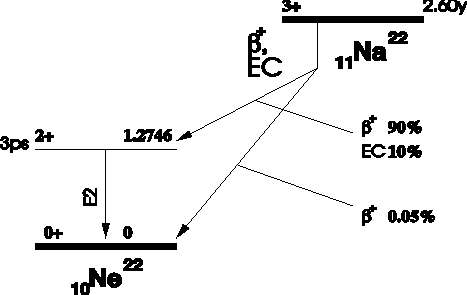
\includegraphics[]{pdf/22Na}
    \end{adjustbox}
    \captionof{figure}{Decay scheme of $^{22}\text{Na}$}
    \label{fig:22NaDecayScheme}
\end{center}
%
\begin{center}
    \begin{adjustbox}{max width=\linewidth, keepaspectratio}
        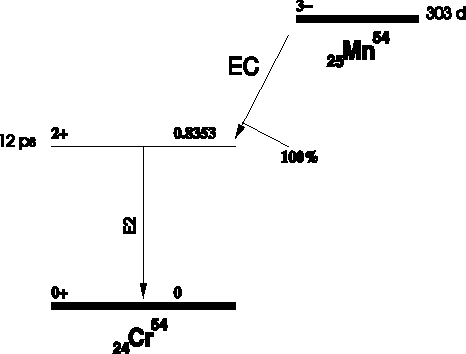
\includegraphics[]{pdf/54Mn}
    \end{adjustbox}
    \captionof{figure}{Decay scheme of $^{54}\text{Mn}$}
    \label{fig:54MnDecayScheme}
\end{center}
%
\begin{center}
    \begin{adjustbox}{max width=\linewidth, keepaspectratio}
        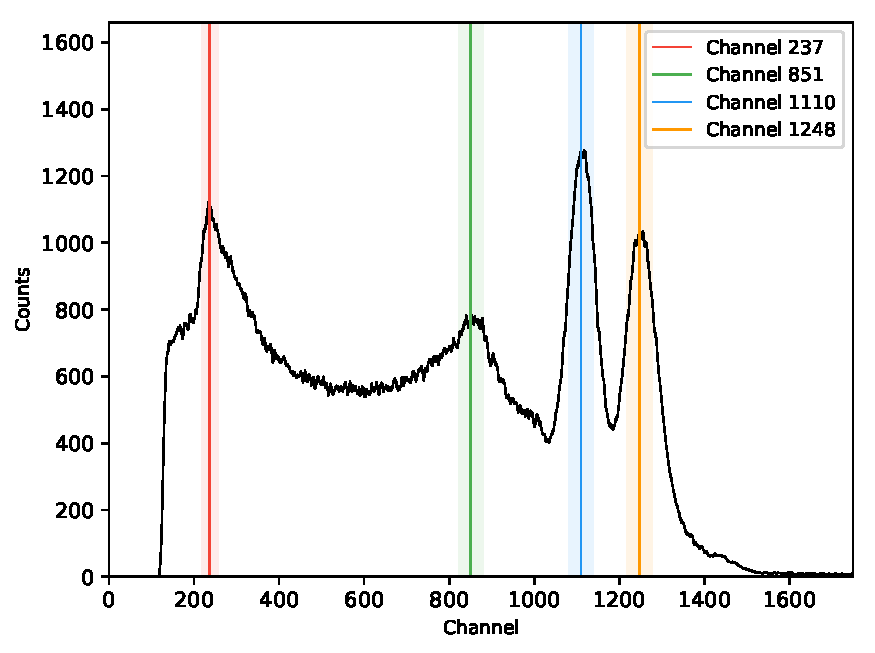
\includegraphics[]{pdf/60Co}
    \end{adjustbox}
    \captionof{figure}{Decay scheme of $^{60}\text{Co}$}
    \label{fig:60CoDecayScheme}
\end{center}
%
\begin{center}
    \begin{adjustbox}{max width=\linewidth, keepaspectratio}
        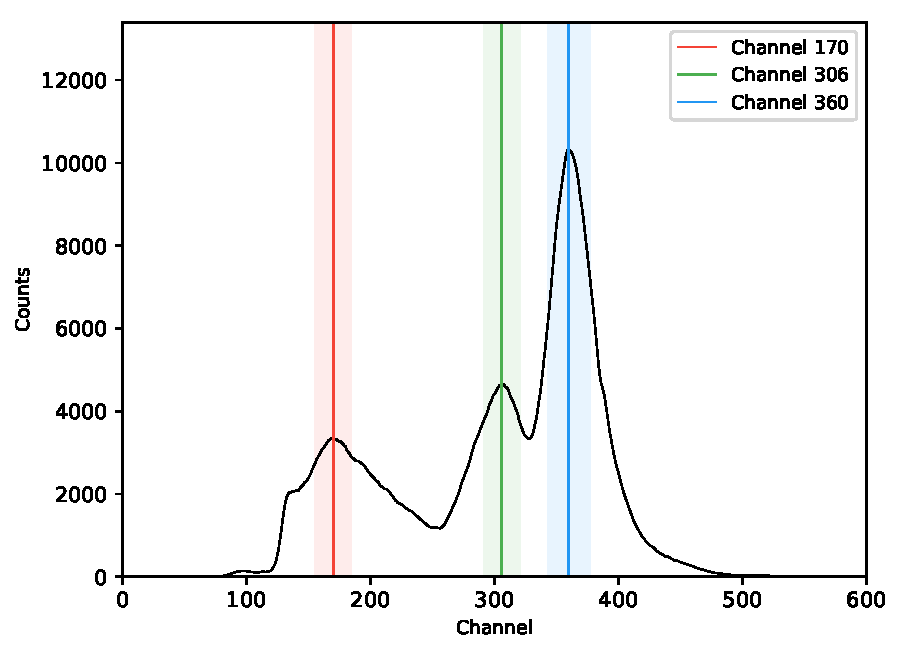
\includegraphics[]{pdf/133Ba}
    \end{adjustbox}
    \captionof{figure}{Decay scheme of $^{133}\text{Ba}$}
    \label{fig:133BaDecayScheme}
\end{center}
%
\begin{center}
    \begin{adjustbox}{max width=\linewidth, keepaspectratio}
        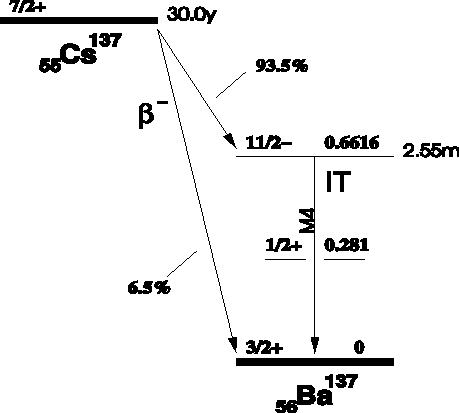
\includegraphics[]{pdf/137Cs}
    \end{adjustbox}
    \captionof{figure}{Decay scheme of $^{137}\text{Cs}$}
    \label{fig:137CsDecayScheme}
\end{center}
%
\subsection{Circuit schematics}
%
\begin{center}
    \begin{adjustbox}{max width=\linewidth, keepaspectratio}
        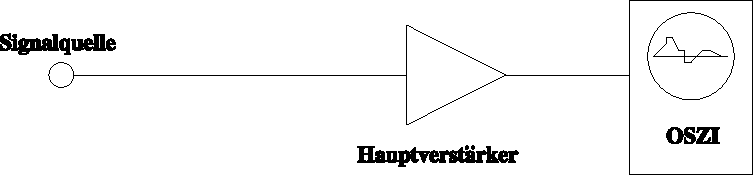
\includegraphics[]{pdf/Schaltung1}
    \end{adjustbox}
    \captionof{figure}{Circuit schematic 1}
    \label{fig:Schaltung1}
\end{center}
%
\begin{center}
    \begin{adjustbox}{max width=\linewidth, keepaspectratio}
        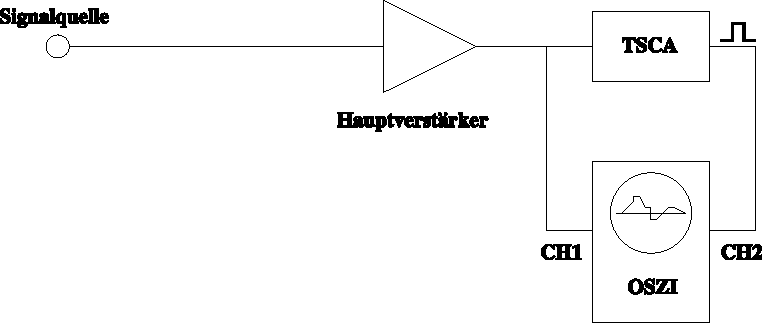
\includegraphics[]{pdf/Schaltung2}
    \end{adjustbox}
    \captionof{figure}{Circuit schematic 2}
    \label{fig:Schaltung2}
\end{center}
%
\begin{center}
    \begin{adjustbox}{max width=\linewidth, keepaspectratio}
        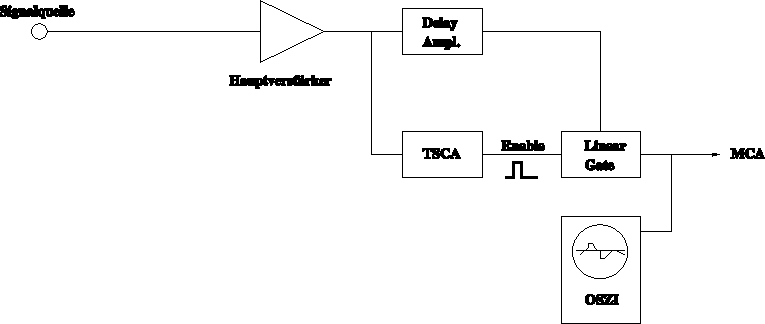
\includegraphics[]{pdf/Schaltung3}
    \end{adjustbox}
    \captionof{figure}{Circuit schematic 3}
    \label{fig:Schaltung3}
\end{center}
%
\begin{center}
    \begin{adjustbox}{max width=\linewidth, keepaspectratio}
        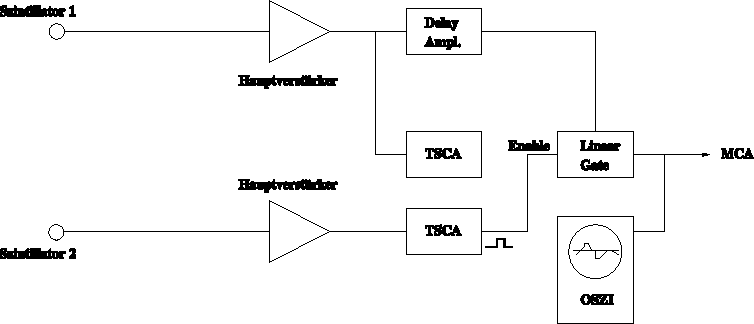
\includegraphics[]{pdf/Schaltung4_mod}
    \end{adjustbox}
    \captionof{figure}{Circuit schematic 4}
    \label{fig:Schaltung4}
\end{center}
%
\begin{center}
    \begin{adjustbox}{max width=\linewidth, keepaspectratio}
        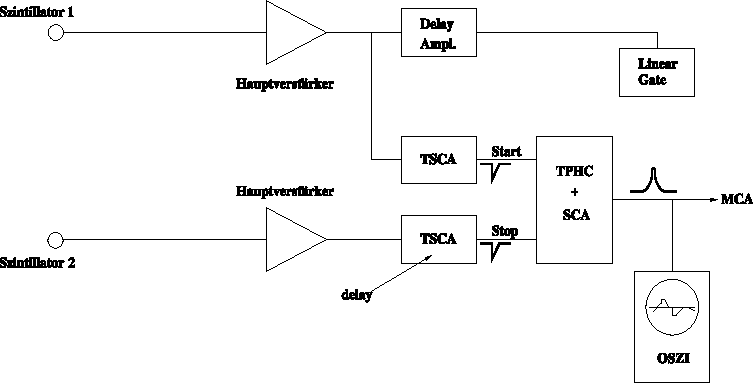
\includegraphics[]{pdf/Schaltung5_mod}
    \end{adjustbox}
    \captionof{figure}{Circuit schematic 5}
    \label{fig:Schaltung5}
\end{center}
%
\begin{center}
    \begin{adjustbox}{max width=\linewidth, keepaspectratio}
        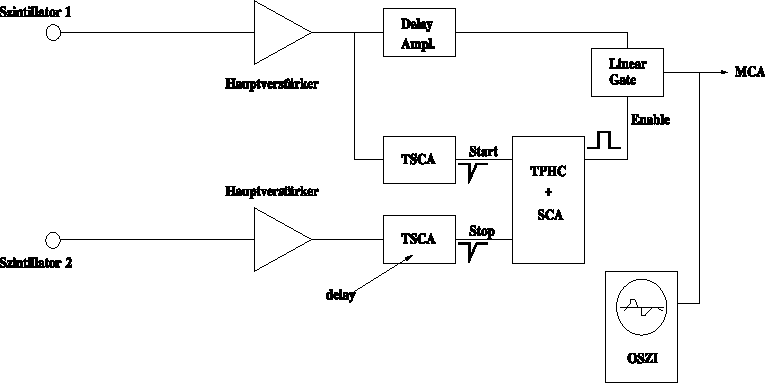
\includegraphics[]{pdf/Schaltung6_mod}
    \end{adjustbox}
    \captionof{figure}{Circuit schematic 6}
    \label{fig:Schaltung6}
\end{center}
%
\subsection{Oscilloscope screenshots}
%
\begin{center}
    \begin{adjustbox}{max width=\linewidth, keepaspectratio}
        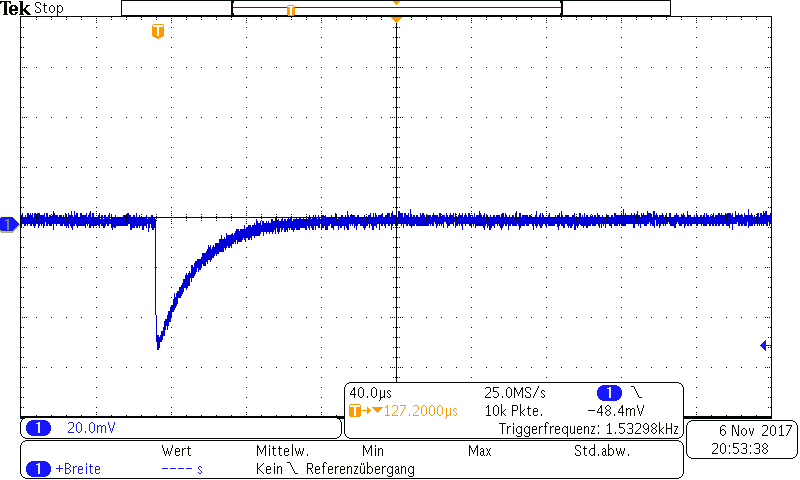
\includegraphics[]{png/tek00000}
    \end{adjustbox}
    \captionof{figure}{}
    \label{fig:}
\end{center}
%
\begin{center}
    \begin{adjustbox}{max width=\linewidth, keepaspectratio}
        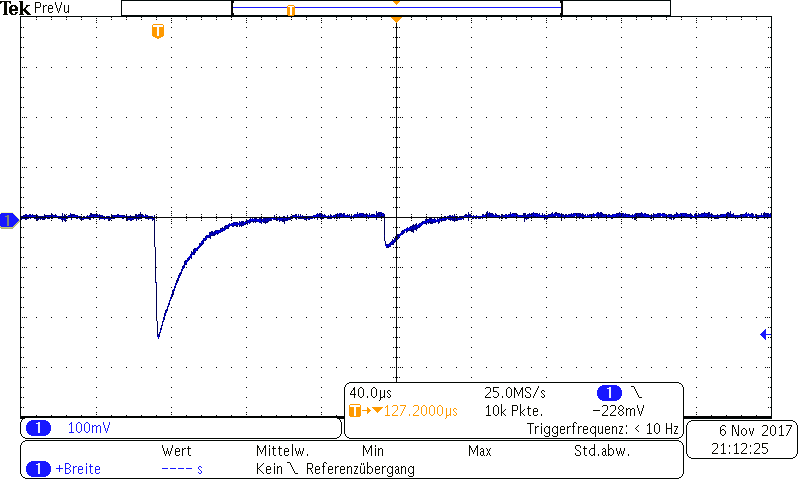
\includegraphics[]{png/tek00001}
    \end{adjustbox}
    \captionof{figure}{}
    \label{fig:}
\end{center}
%
\begin{center}
    \begin{adjustbox}{max width=\linewidth, keepaspectratio}
        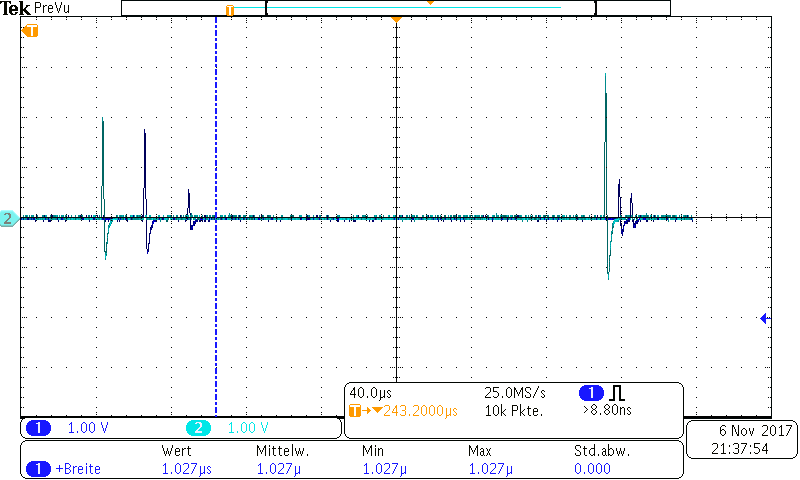
\includegraphics[]{png/tek00003}
    \end{adjustbox}
    \captionof{figure}{}
    \label{fig:}
\end{center}
%
\begin{center}
    \begin{adjustbox}{max width=\linewidth, keepaspectratio}
        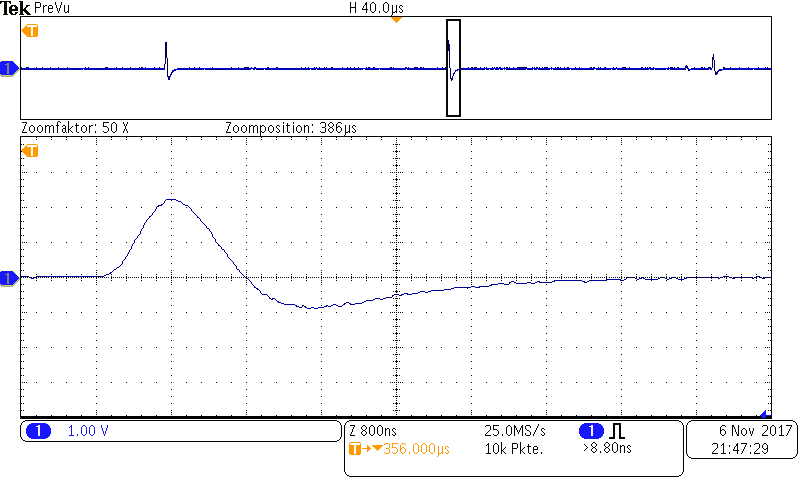
\includegraphics[]{png/tek00004}
    \end{adjustbox}
    \captionof{figure}{}
    \label{fig:}
\end{center}
%
\begin{center}
    \begin{adjustbox}{max width=\linewidth, keepaspectratio}
        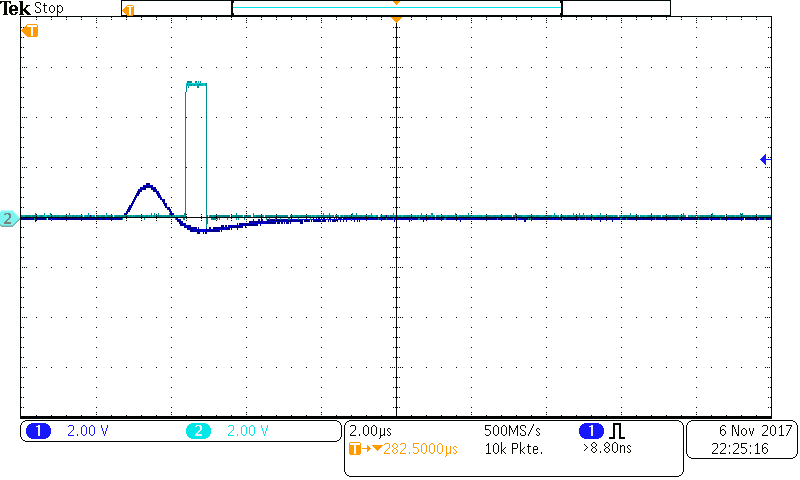
\includegraphics[]{png/tek00006}
    \end{adjustbox}
    \captionof{figure}{}
    \label{fig:}
\end{center}
%
\begin{center}
    \begin{adjustbox}{max width=\linewidth, keepaspectratio}
        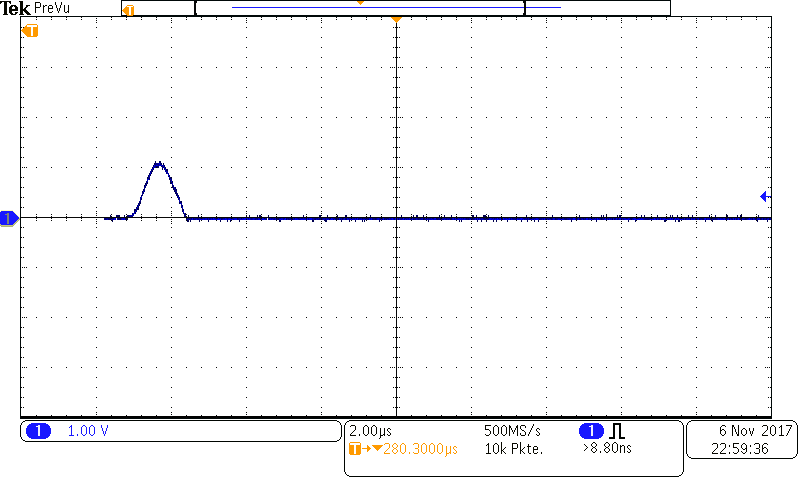
\includegraphics[]{png/tek00007}
    \end{adjustbox}
    \captionof{figure}{}
    \label{fig:}
\end{center}
%
\subsection{Plots}
%
\begin{center}
    \begin{adjustbox}{max width=\linewidth, keepaspectratio}
        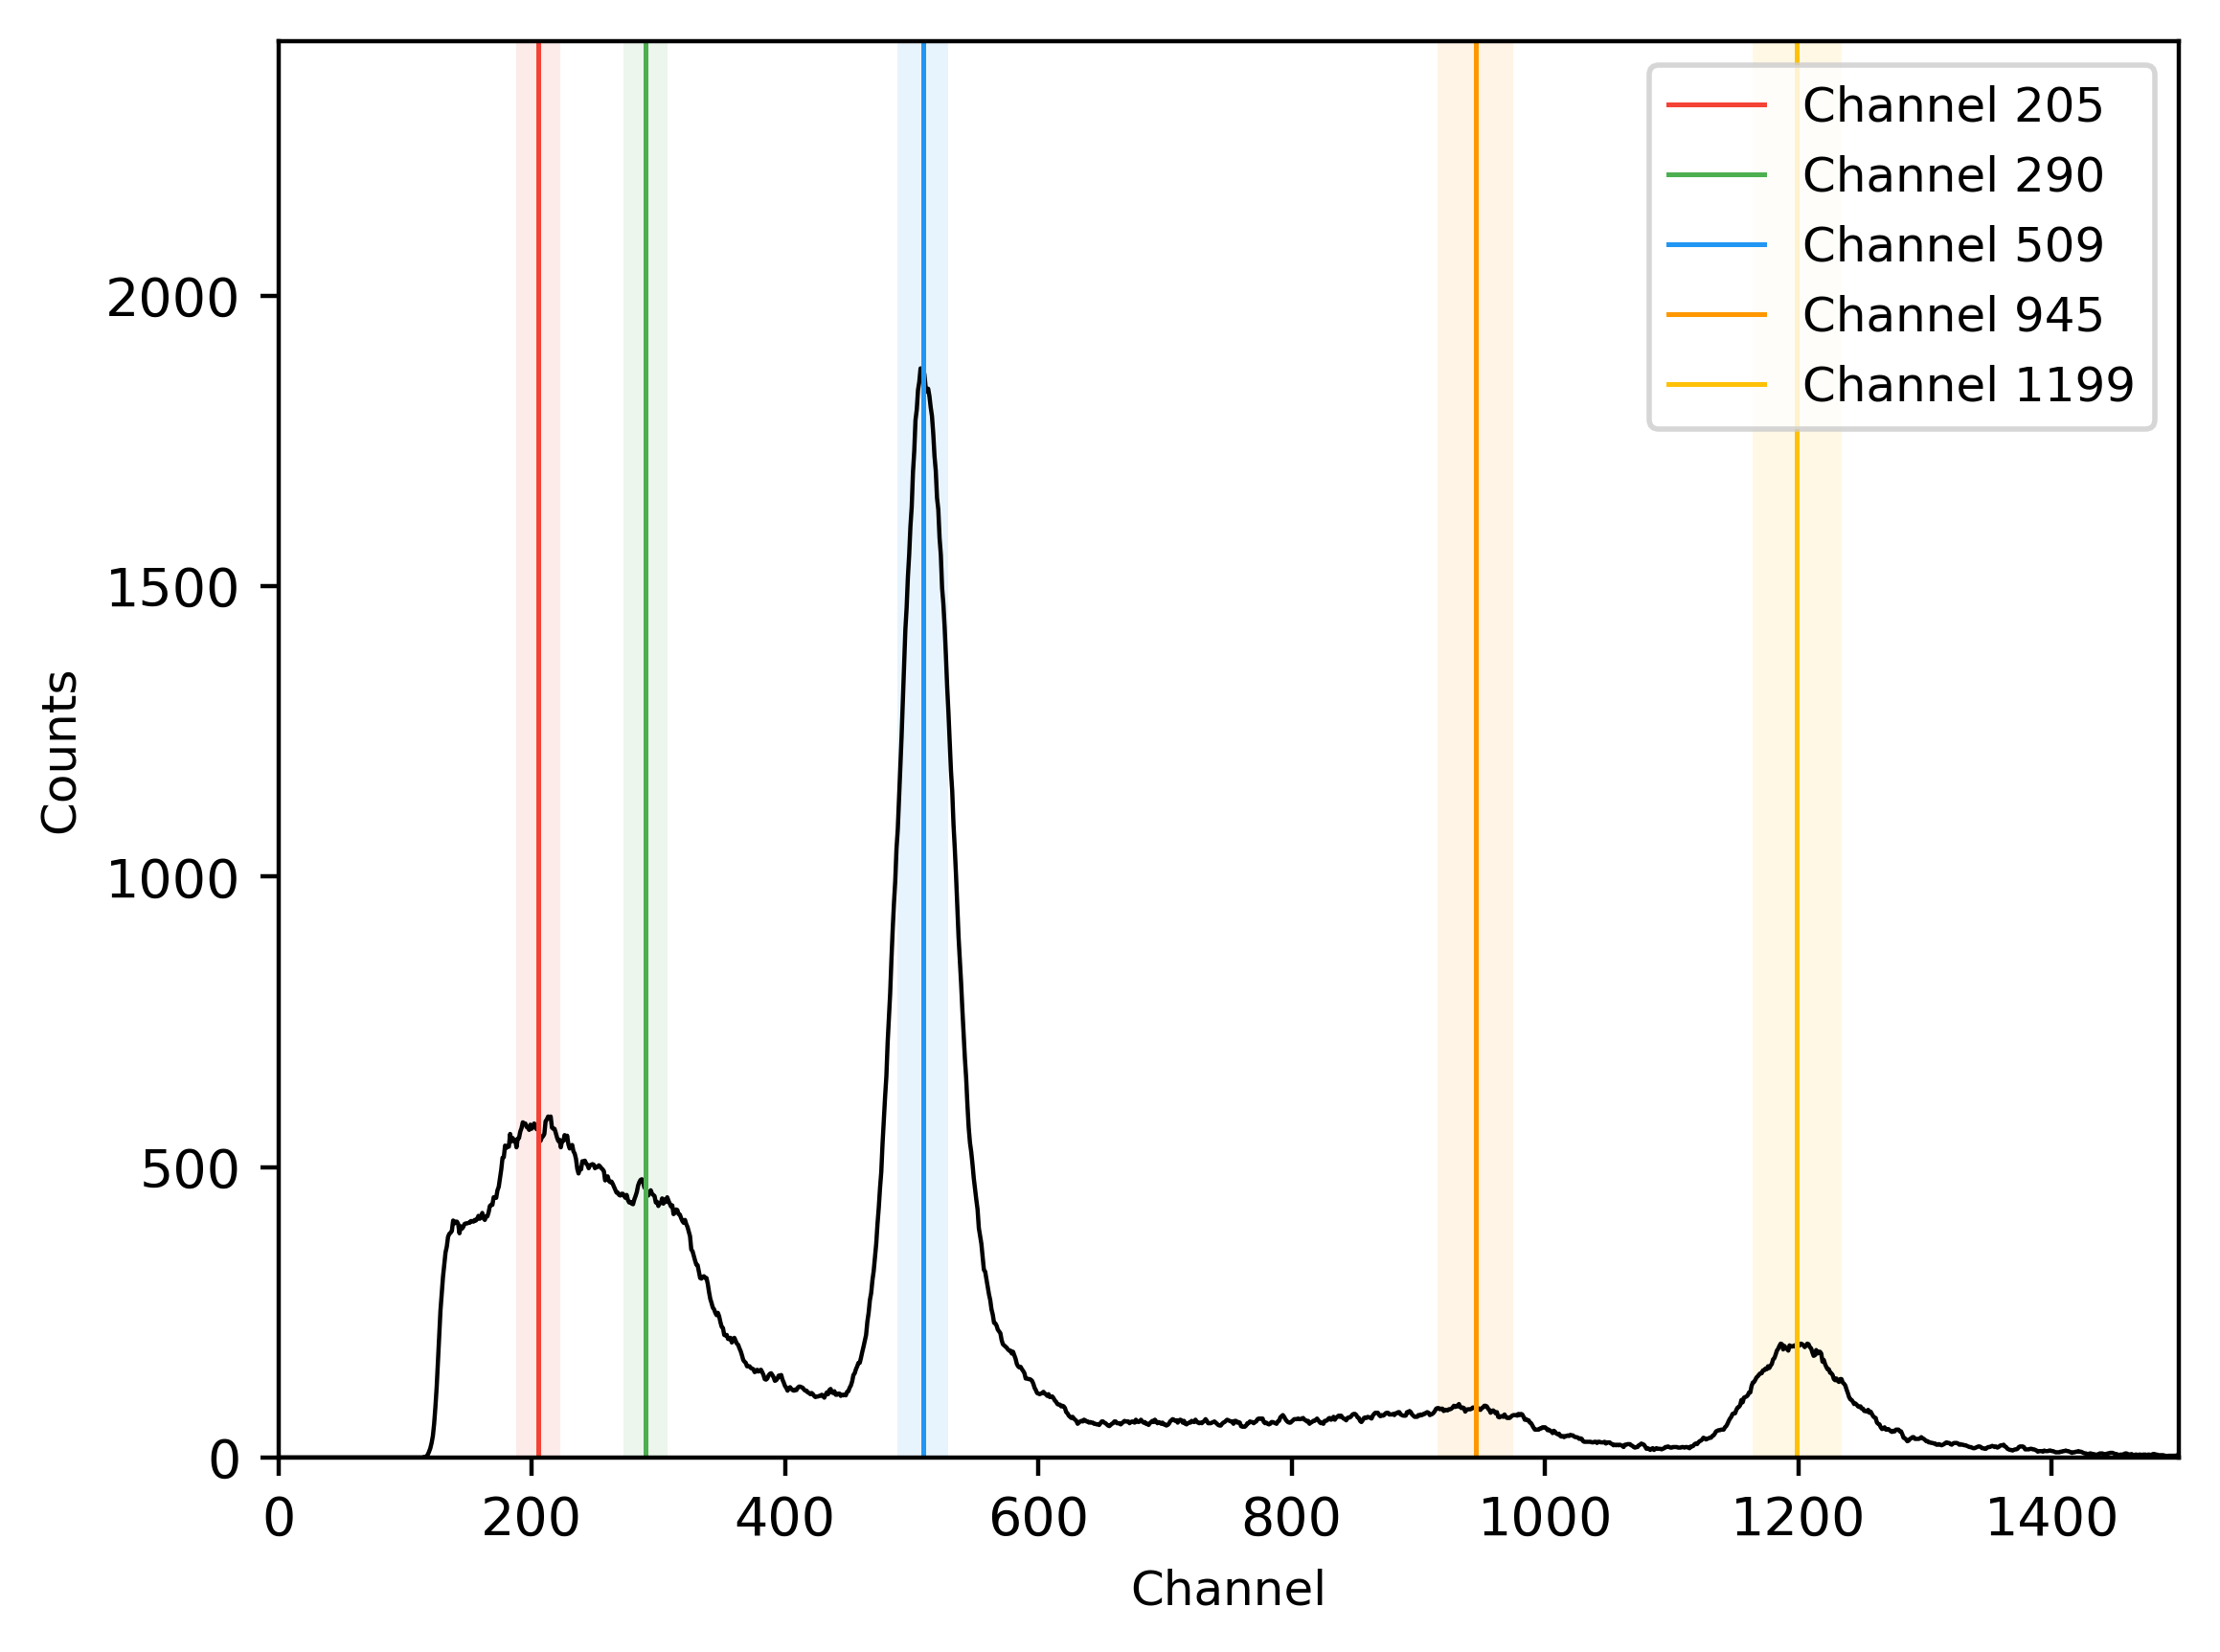
\includegraphics[]{png/22Na}
    \end{adjustbox}
    \captionof{figure}{22Na}
    \label{fig:}
\end{center}
%
\begin{center}
    \begin{adjustbox}{max width=\linewidth, keepaspectratio}
        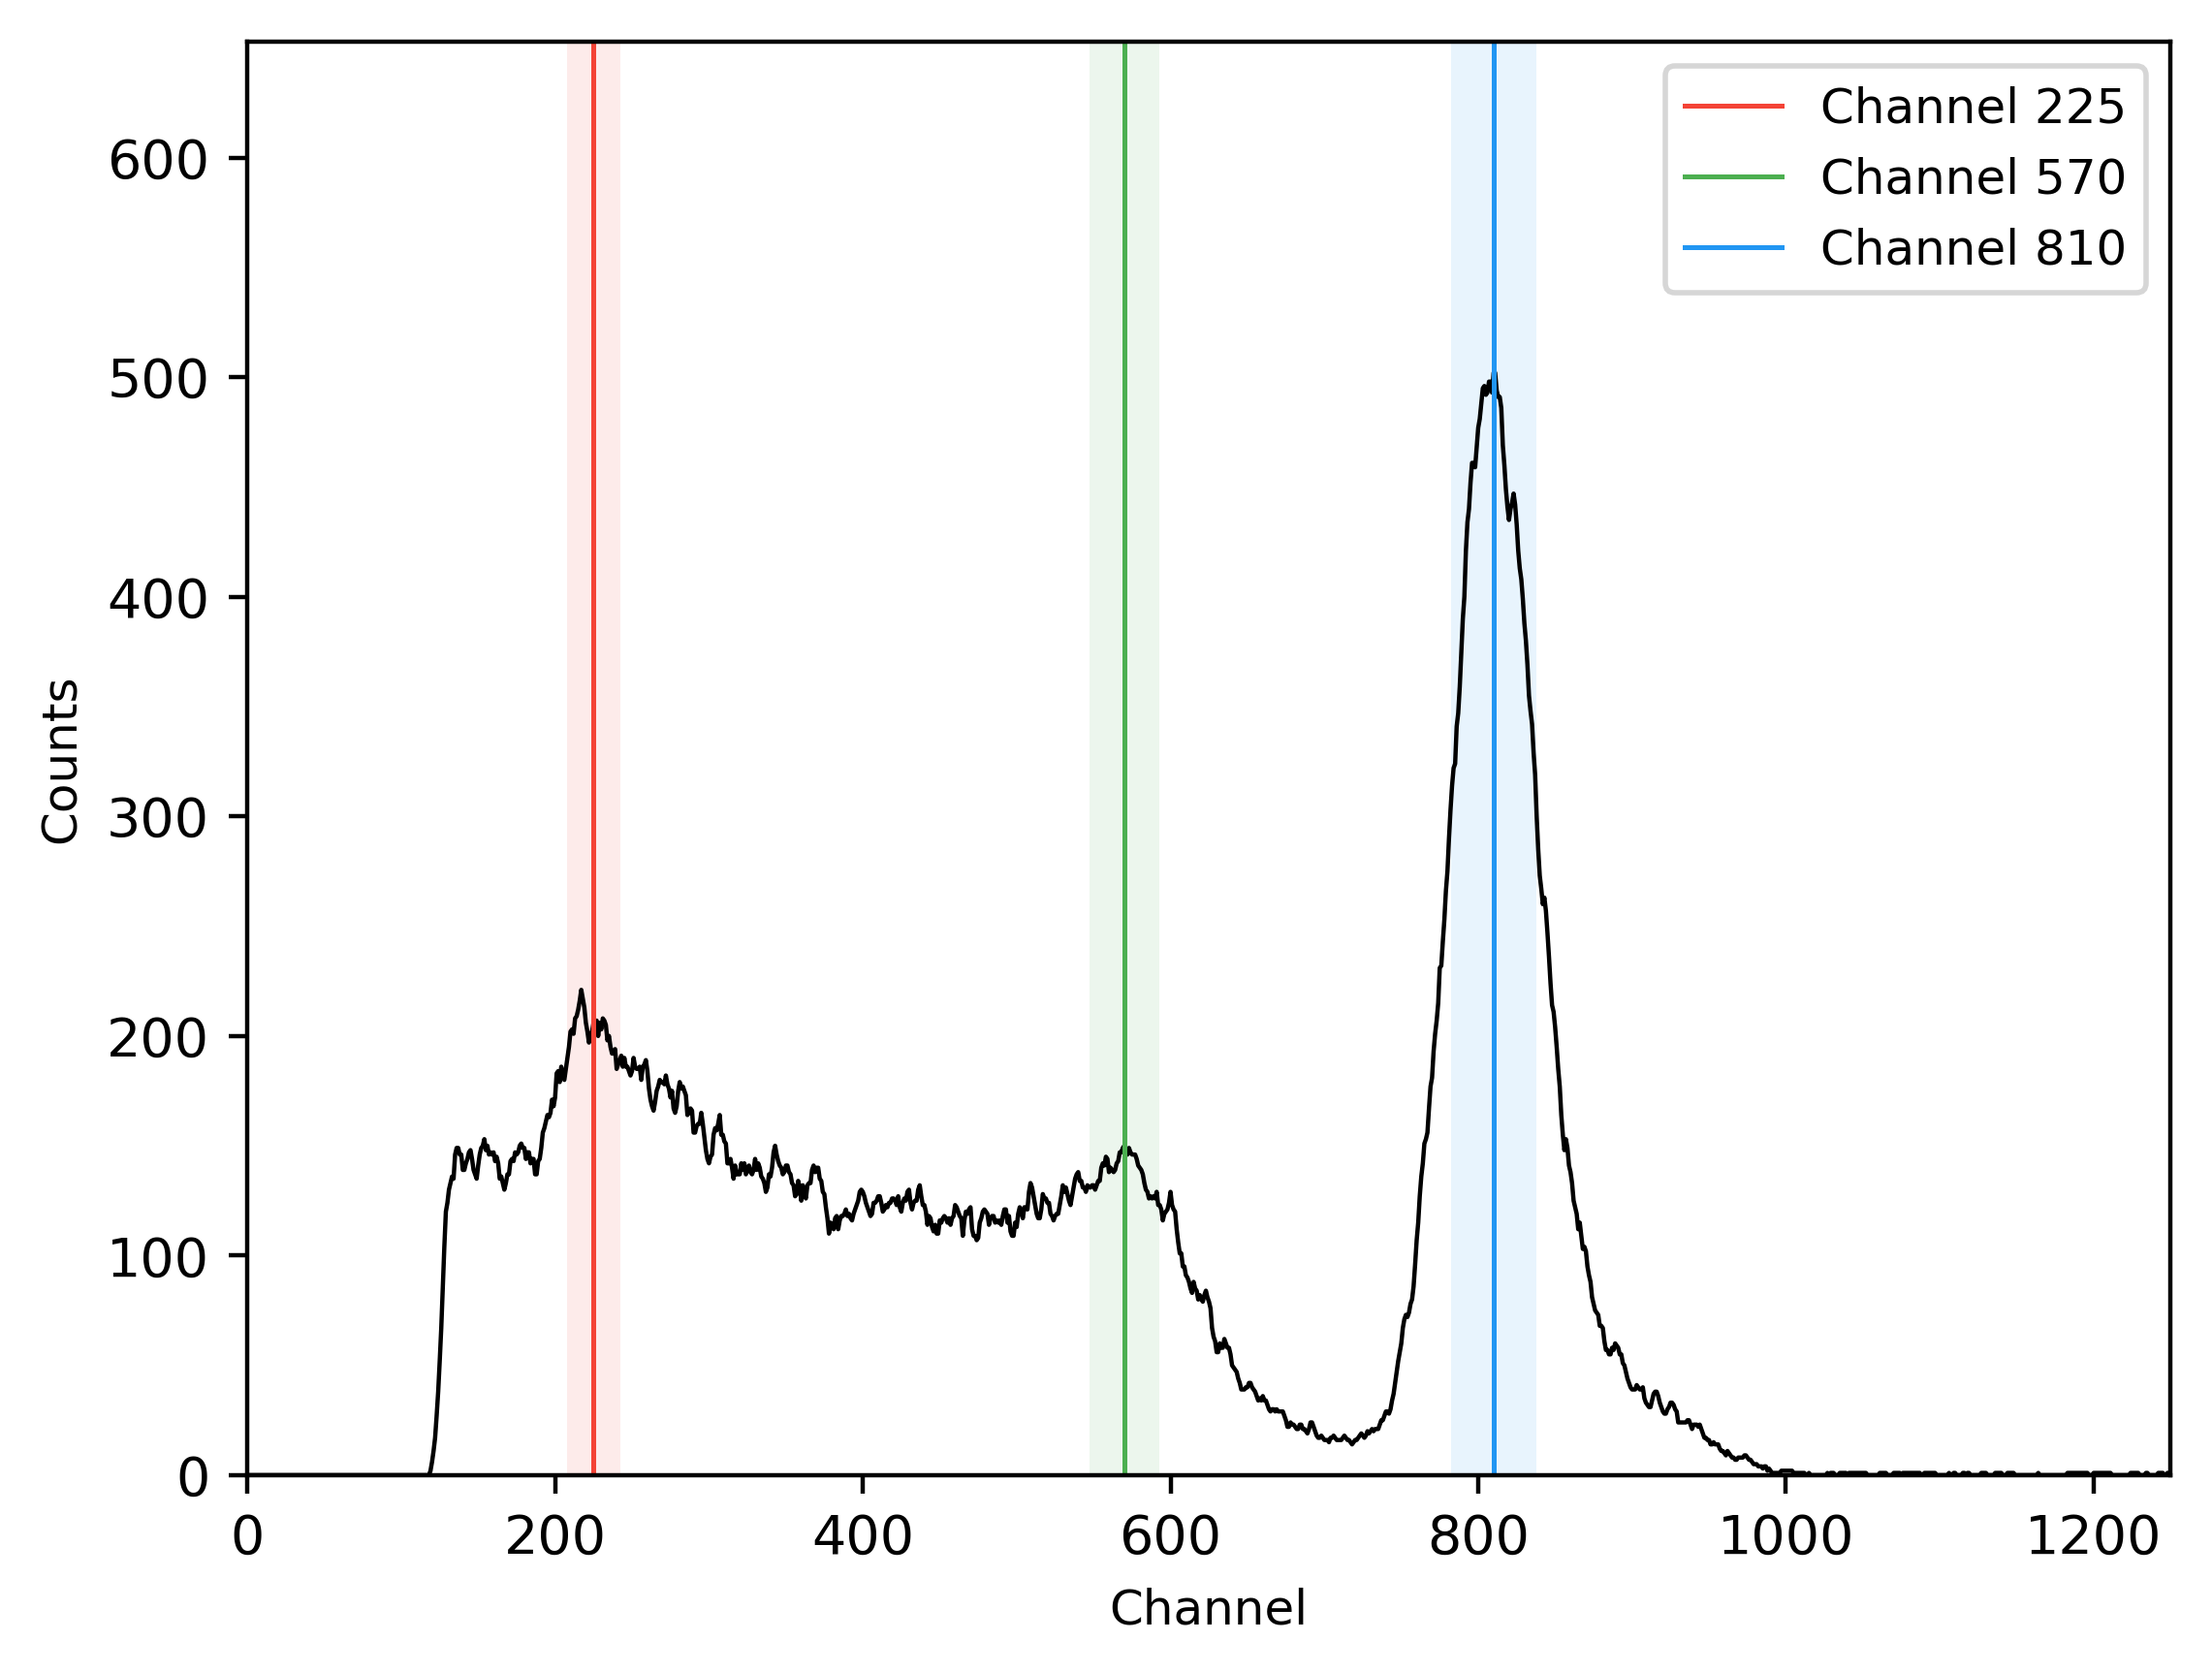
\includegraphics[]{png/54Mn}
    \end{adjustbox}
    \captionof{figure}{54Mn}
    \label{fig:}
\end{center}
%
\begin{center}
    \begin{adjustbox}{max width=\linewidth, keepaspectratio}
        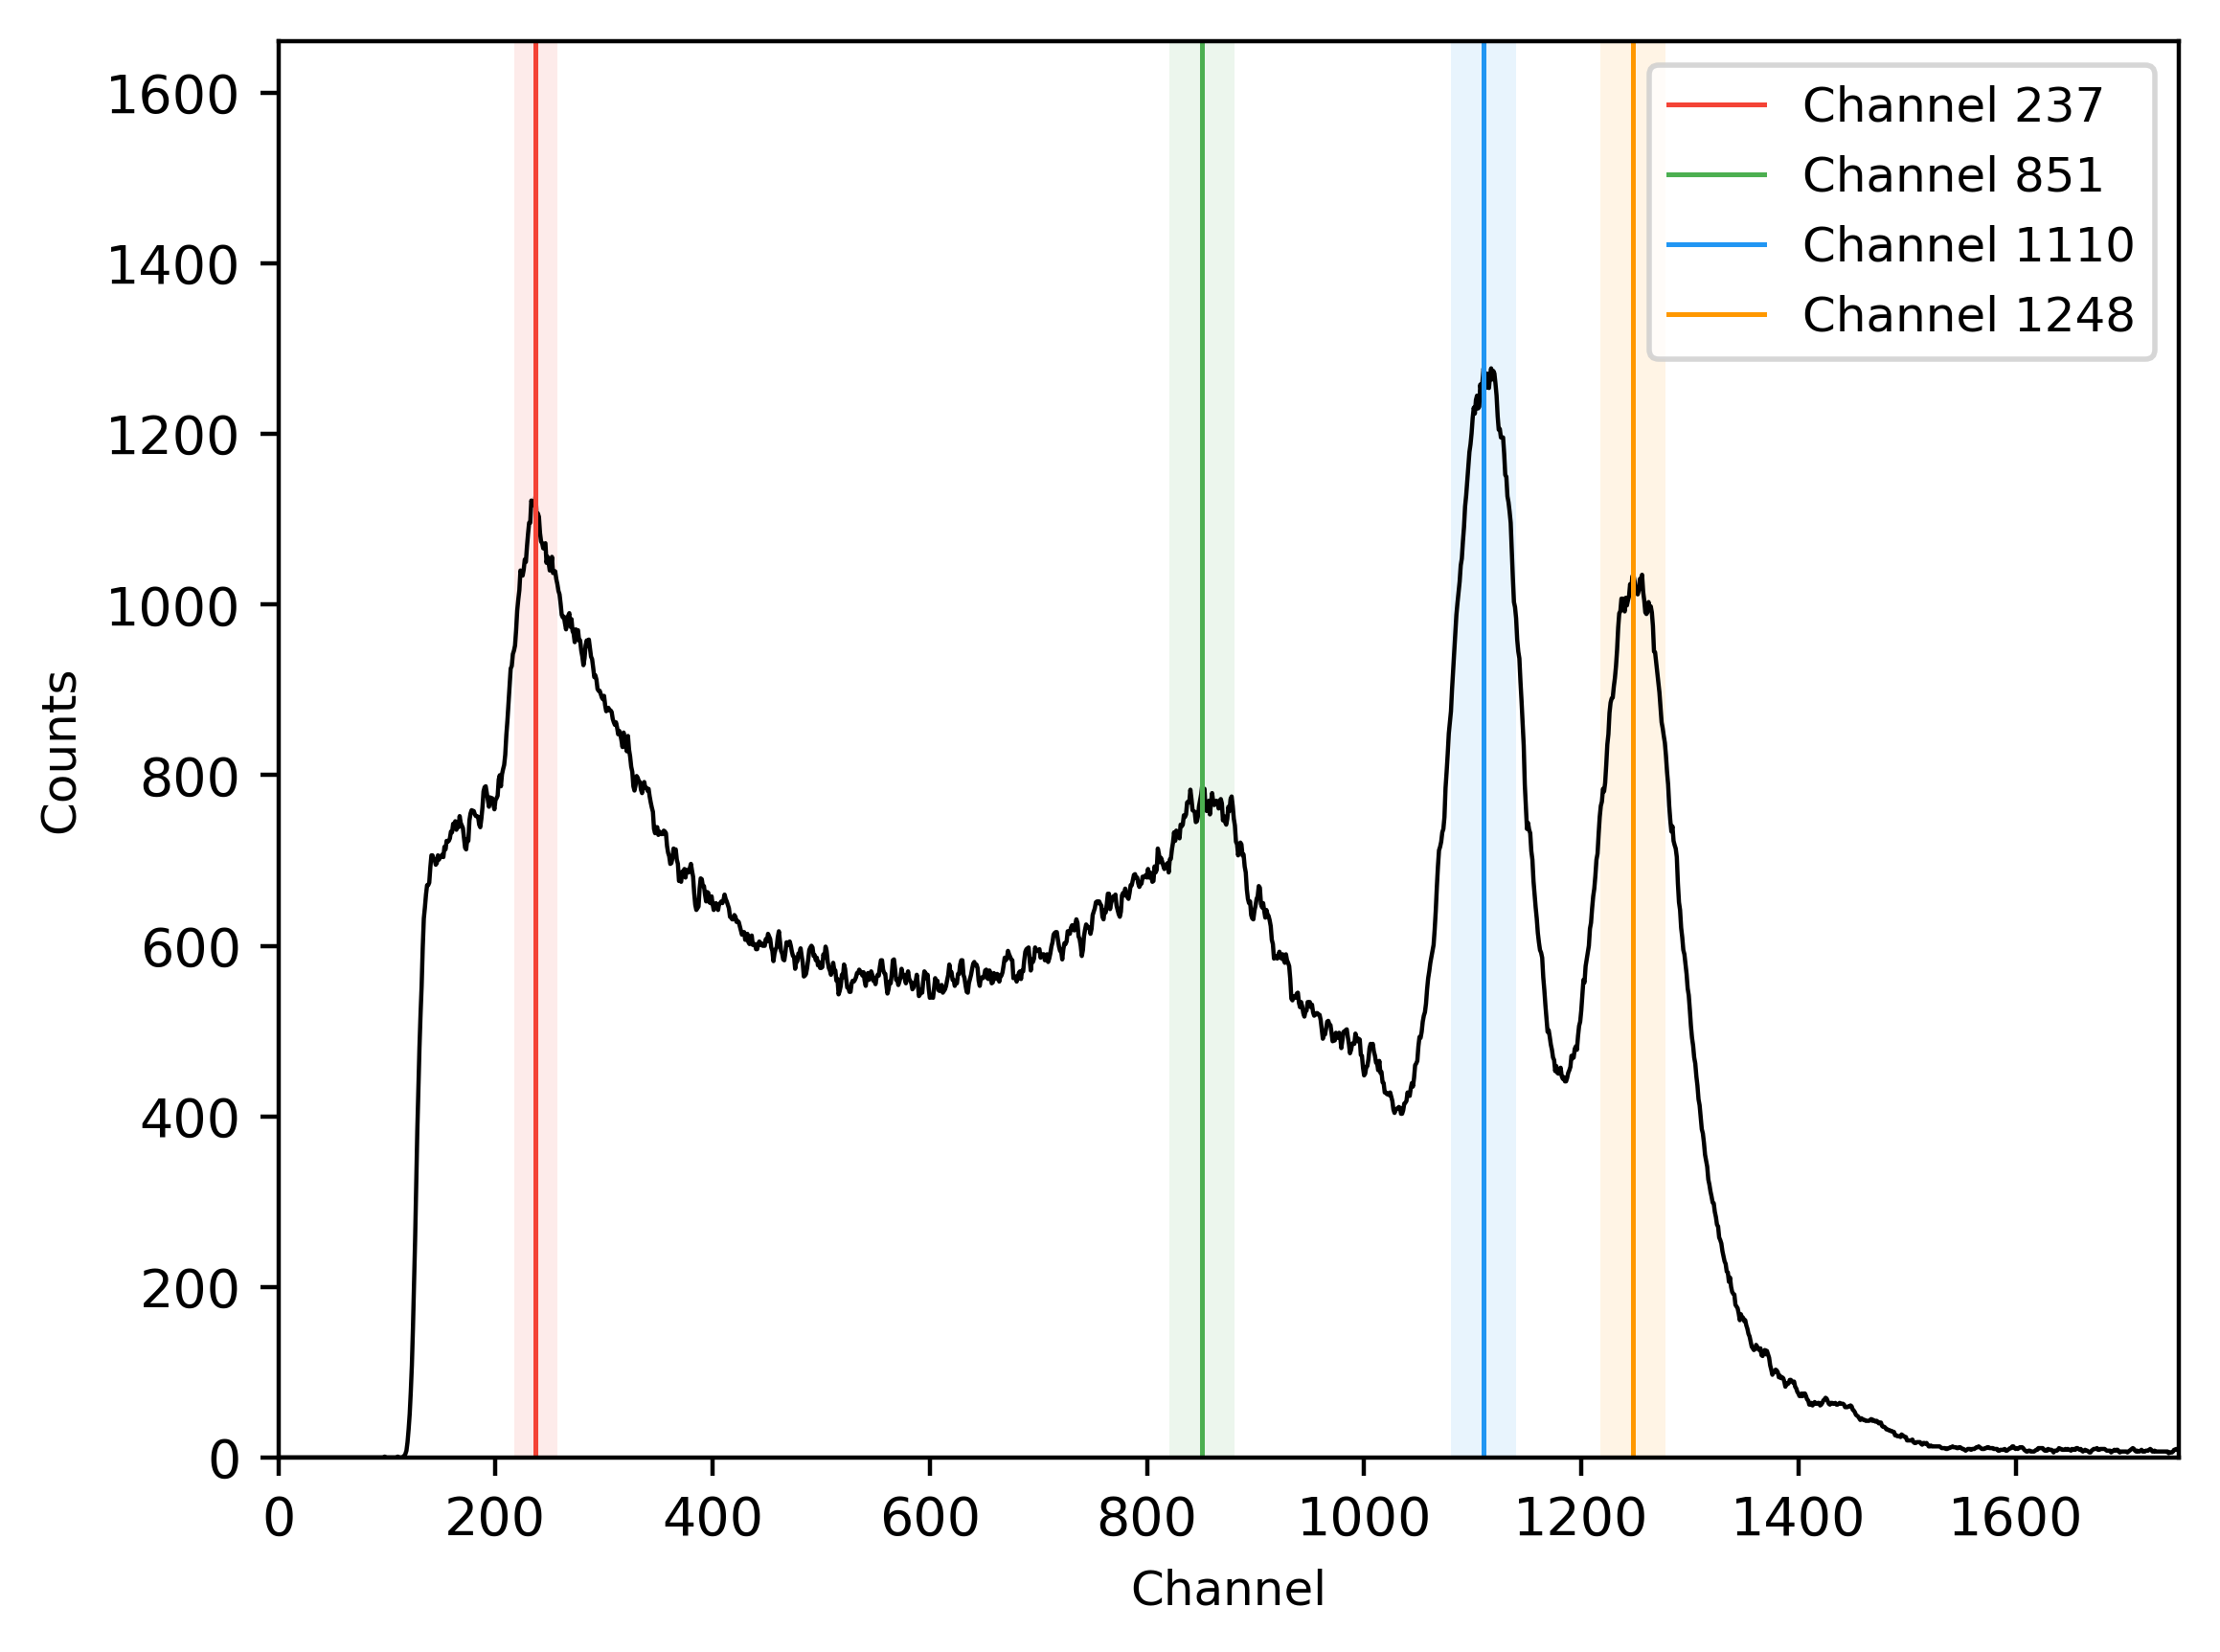
\includegraphics[]{png/60Co}
    \end{adjustbox}
    \captionof{figure}{60Co}
    \label{fig:}
\end{center}
%
\begin{center}
    \begin{adjustbox}{max width=\linewidth, keepaspectratio}
        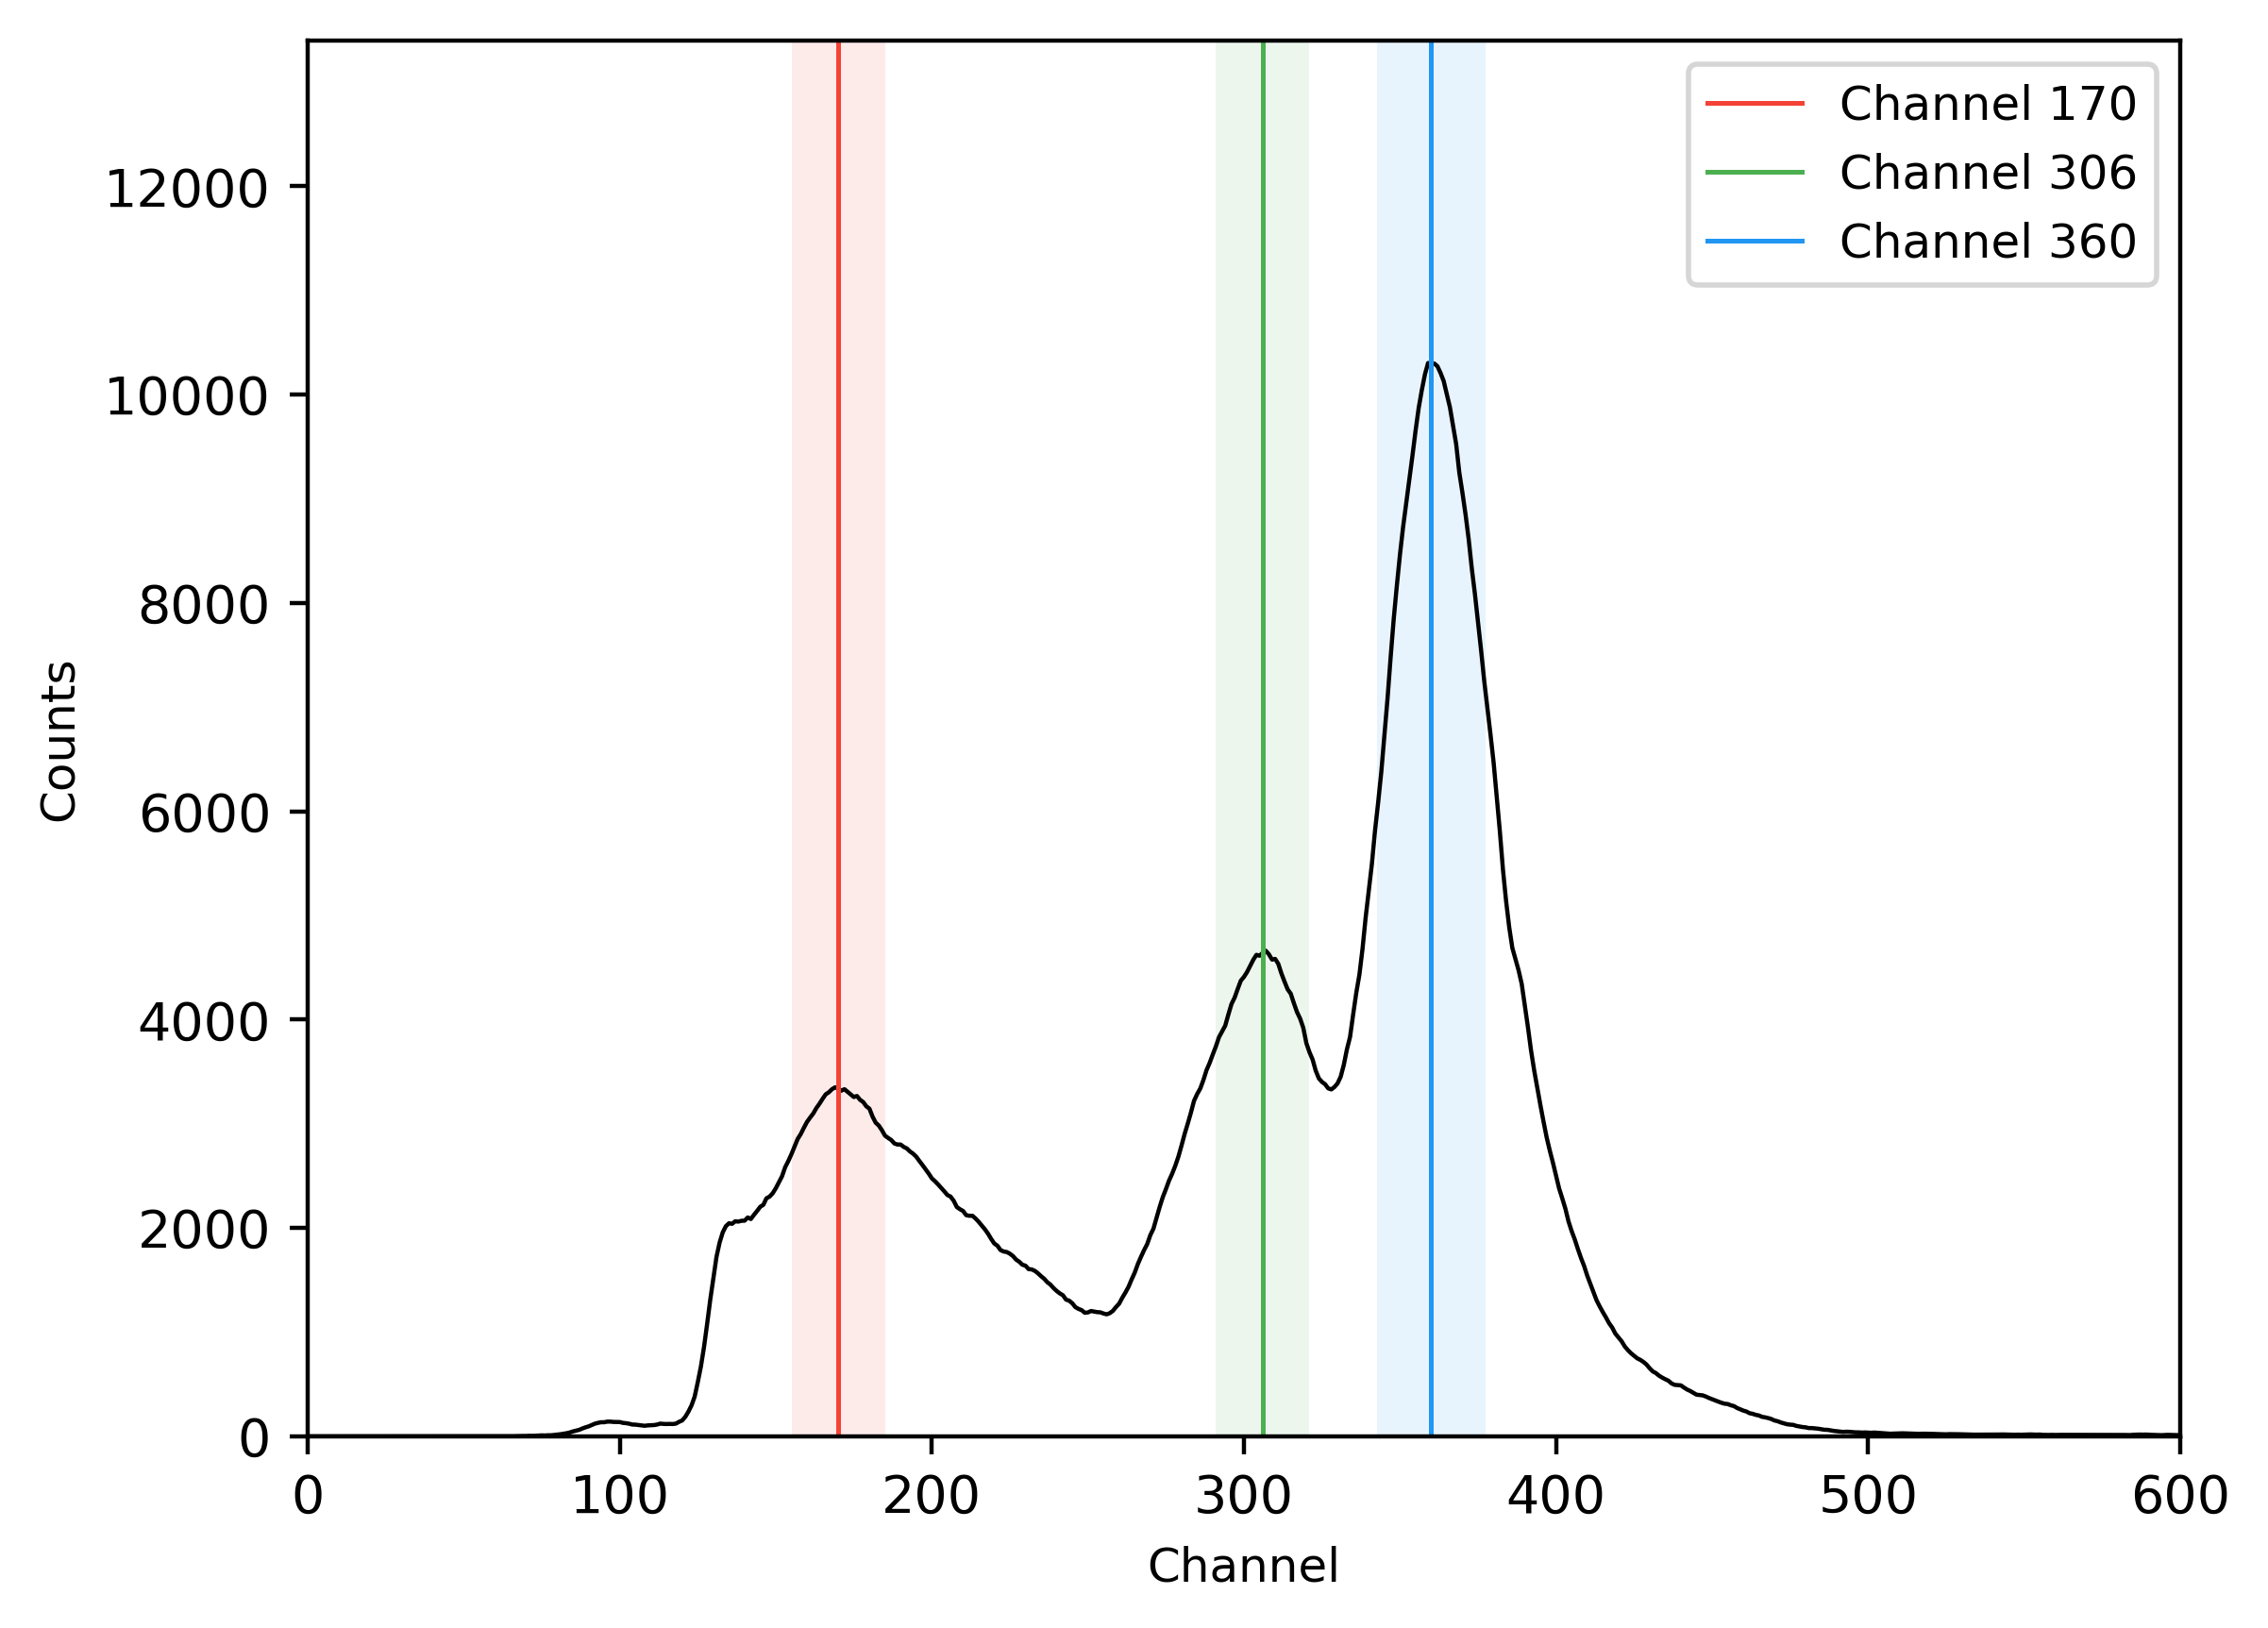
\includegraphics[]{png/133Ba}
    \end{adjustbox}
    \captionof{figure}{133Ba}
    \label{fig:}
\end{center}
%
\begin{center}
    \begin{adjustbox}{max width=\linewidth, keepaspectratio}
        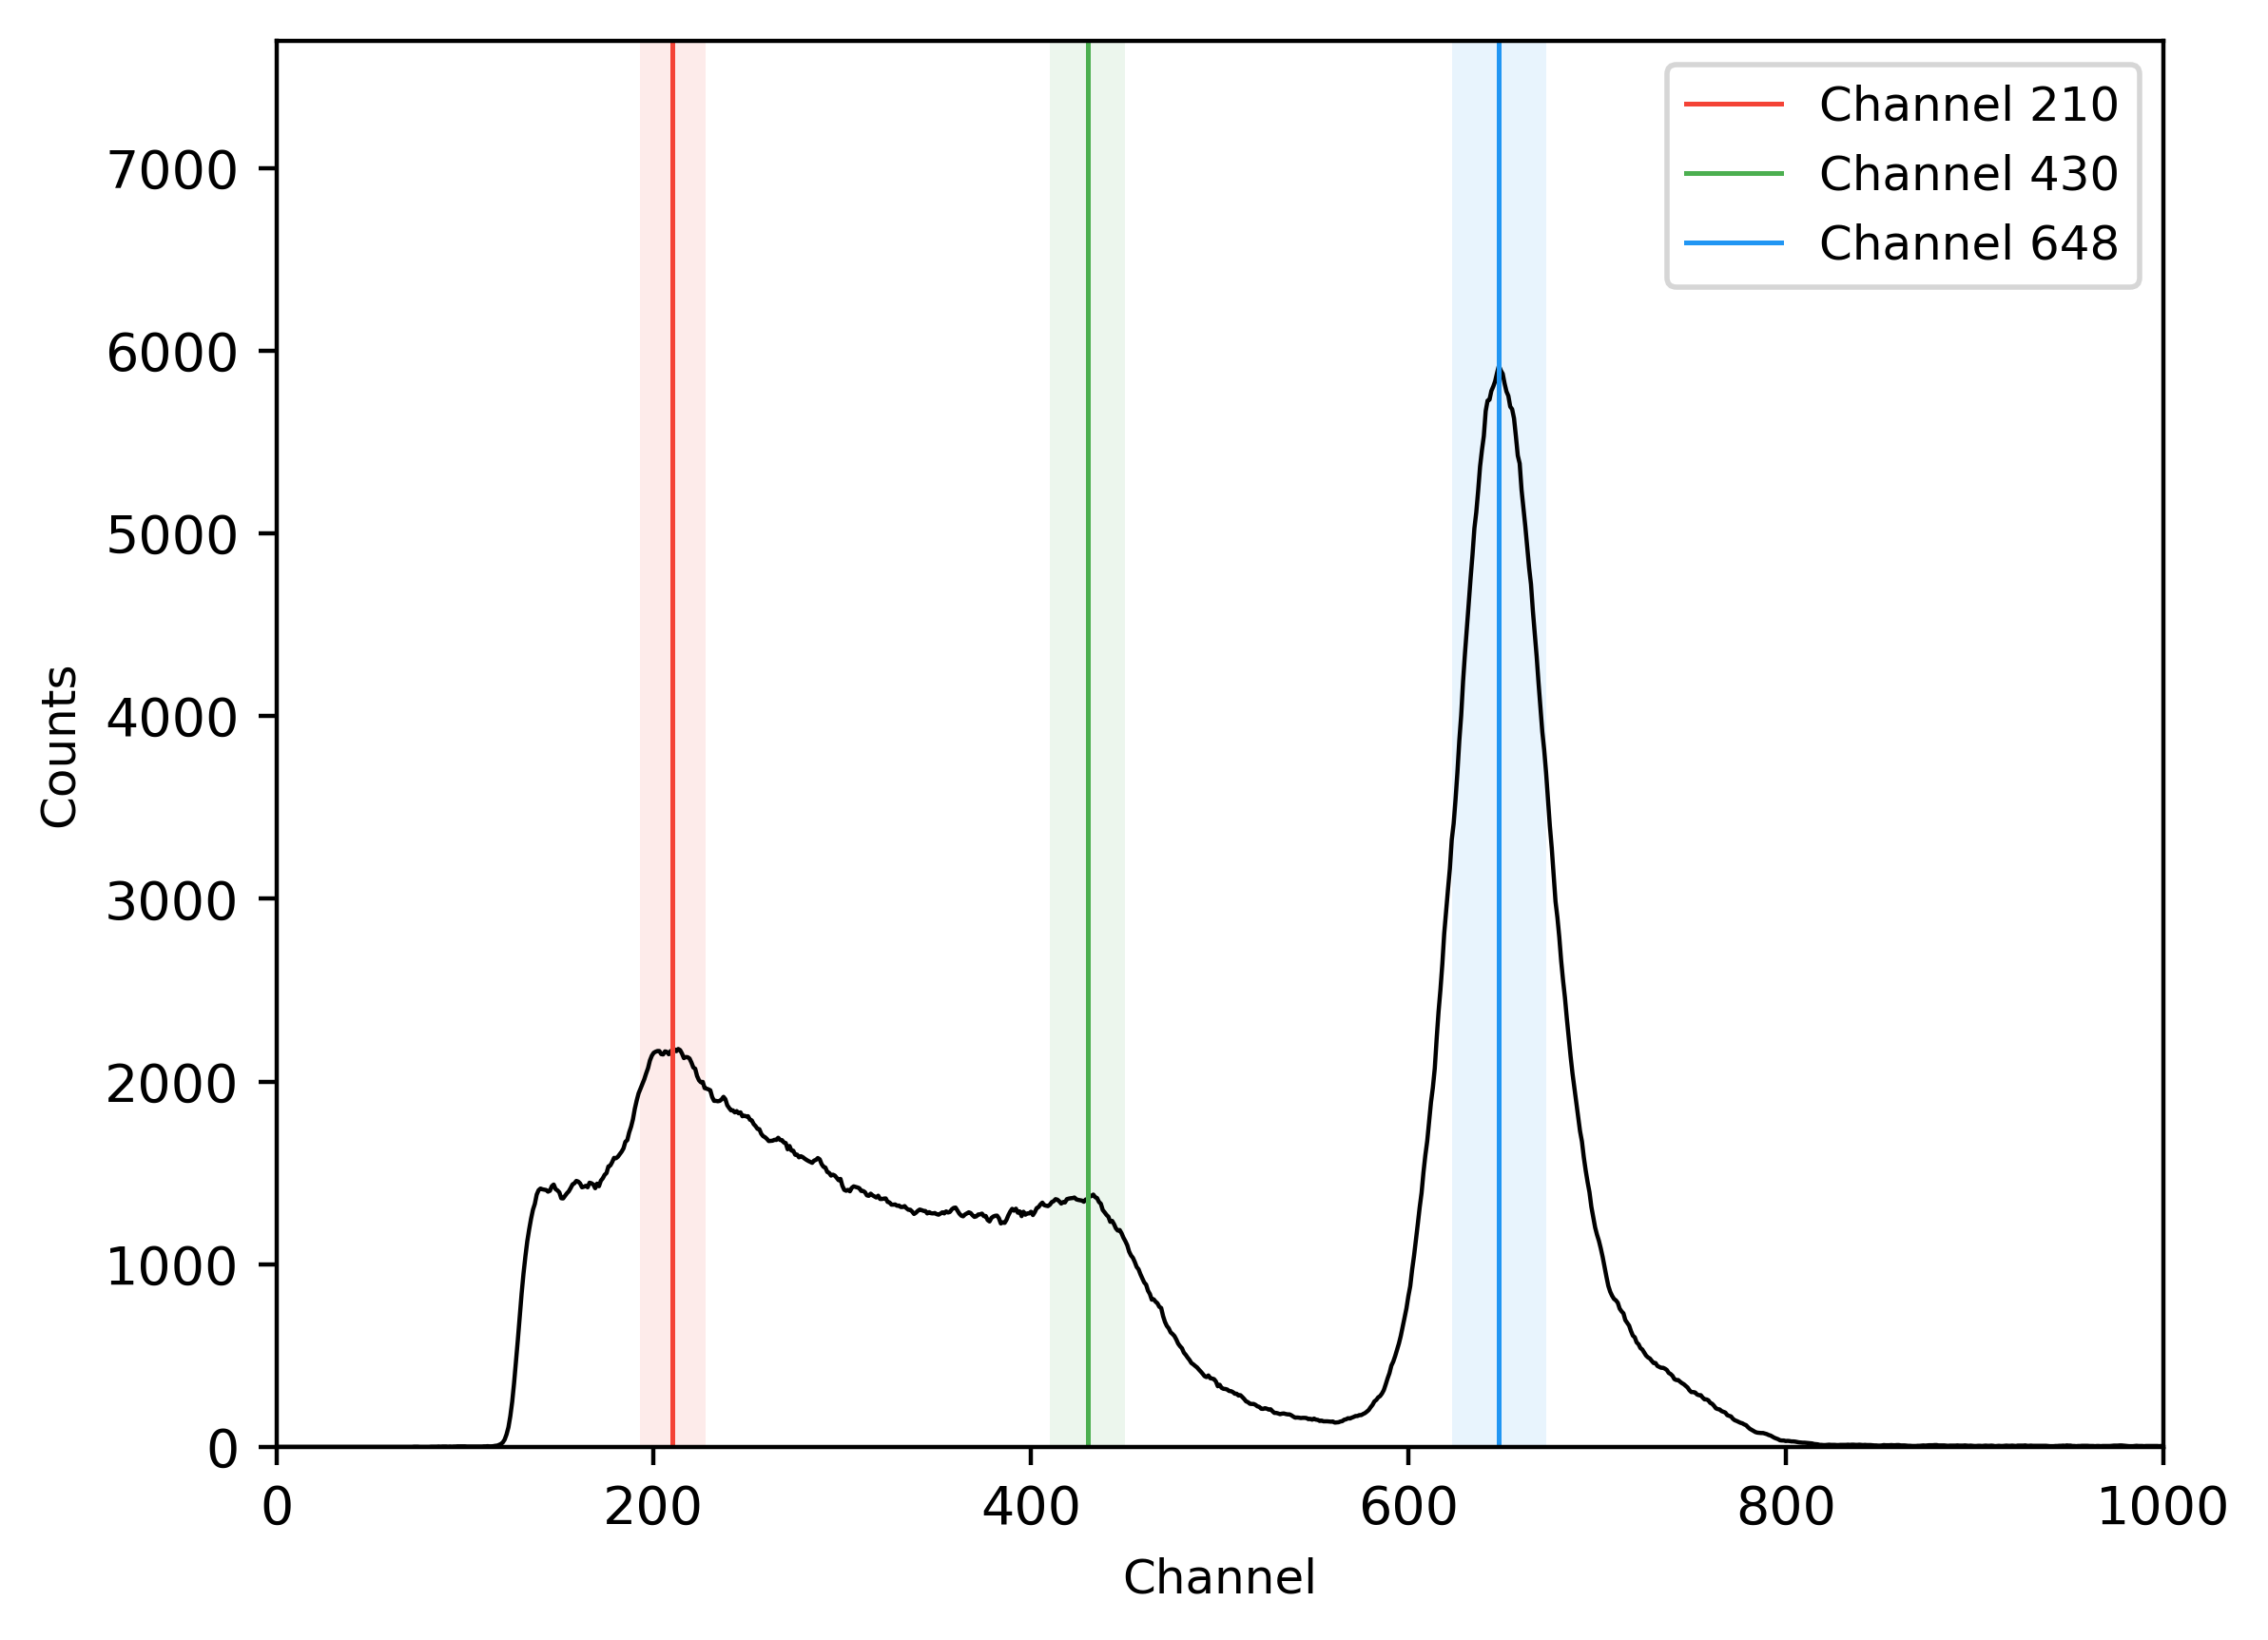
\includegraphics[]{png/137Cs}
    \end{adjustbox}
    \captionof{figure}{137Cs}
    \label{fig:}
\end{center}
%
\begin{center}
    \begin{adjustbox}{max width=\linewidth, keepaspectratio}
        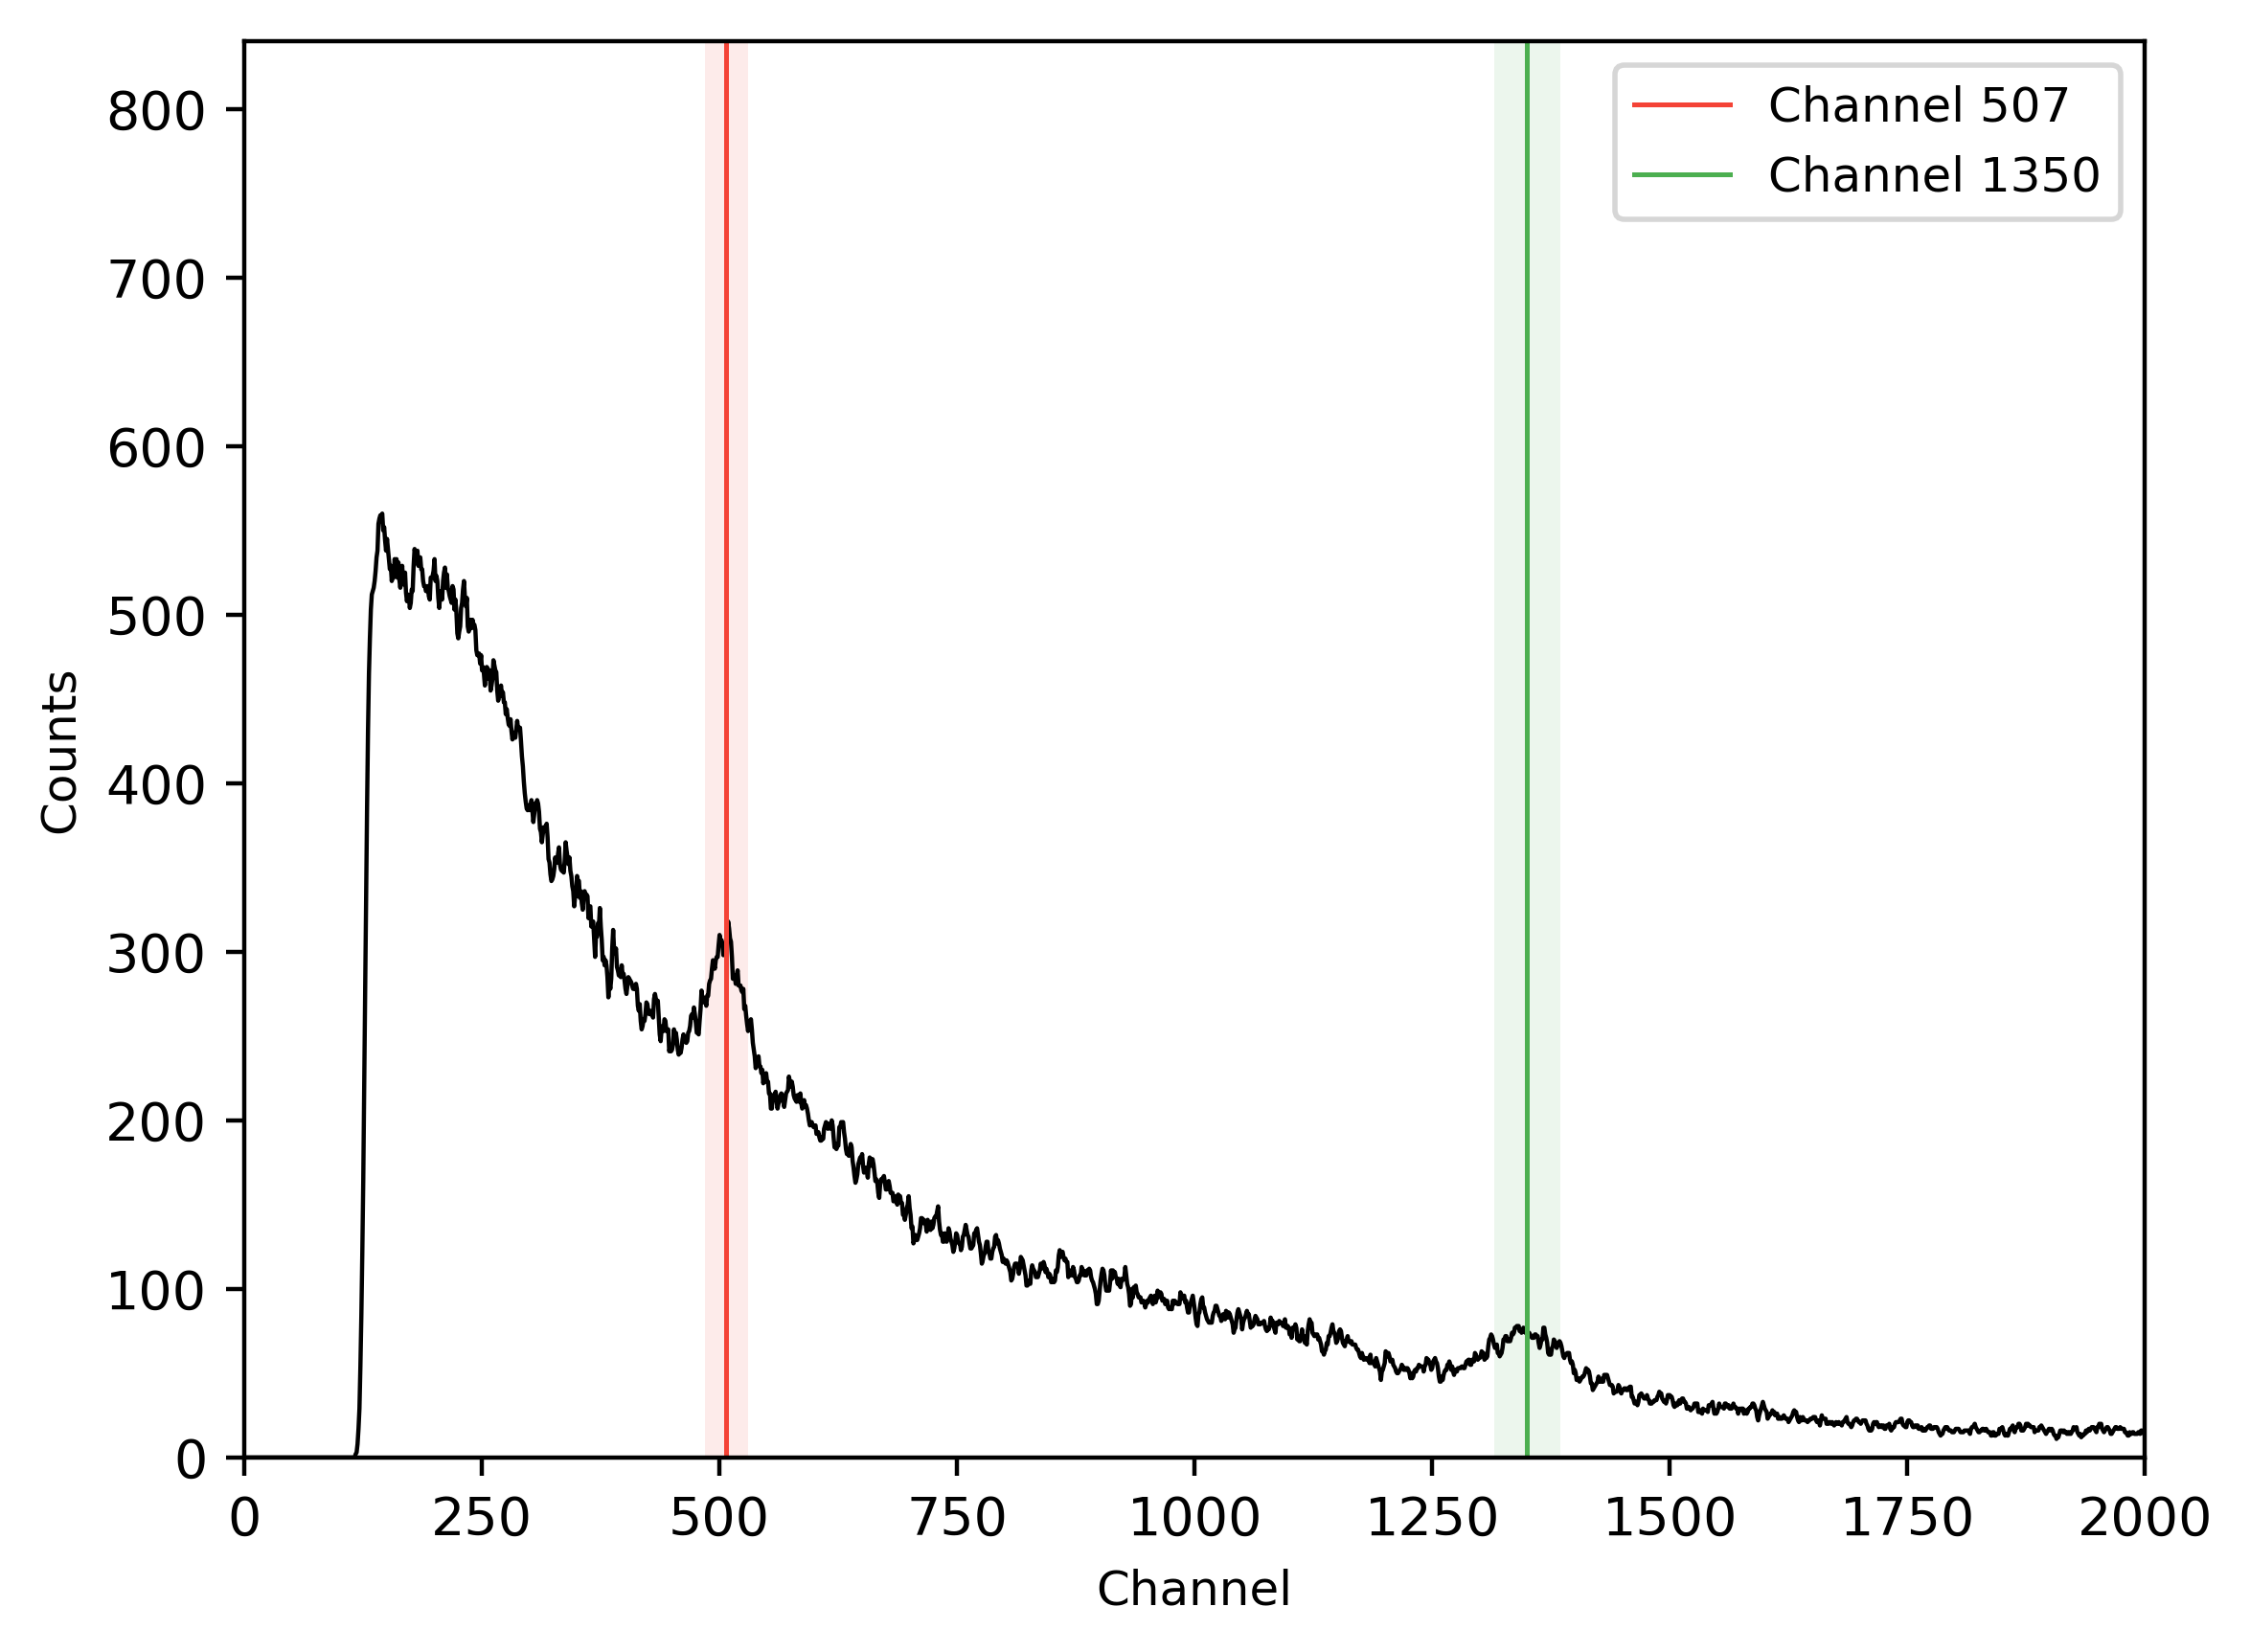
\includegraphics[]{png/night}
    \end{adjustbox}
    \captionof{figure}{night}
    \label{fig:}
\end{center}
%
\begin{center}
    \begin{adjustbox}{max width=\linewidth, keepaspectratio}
        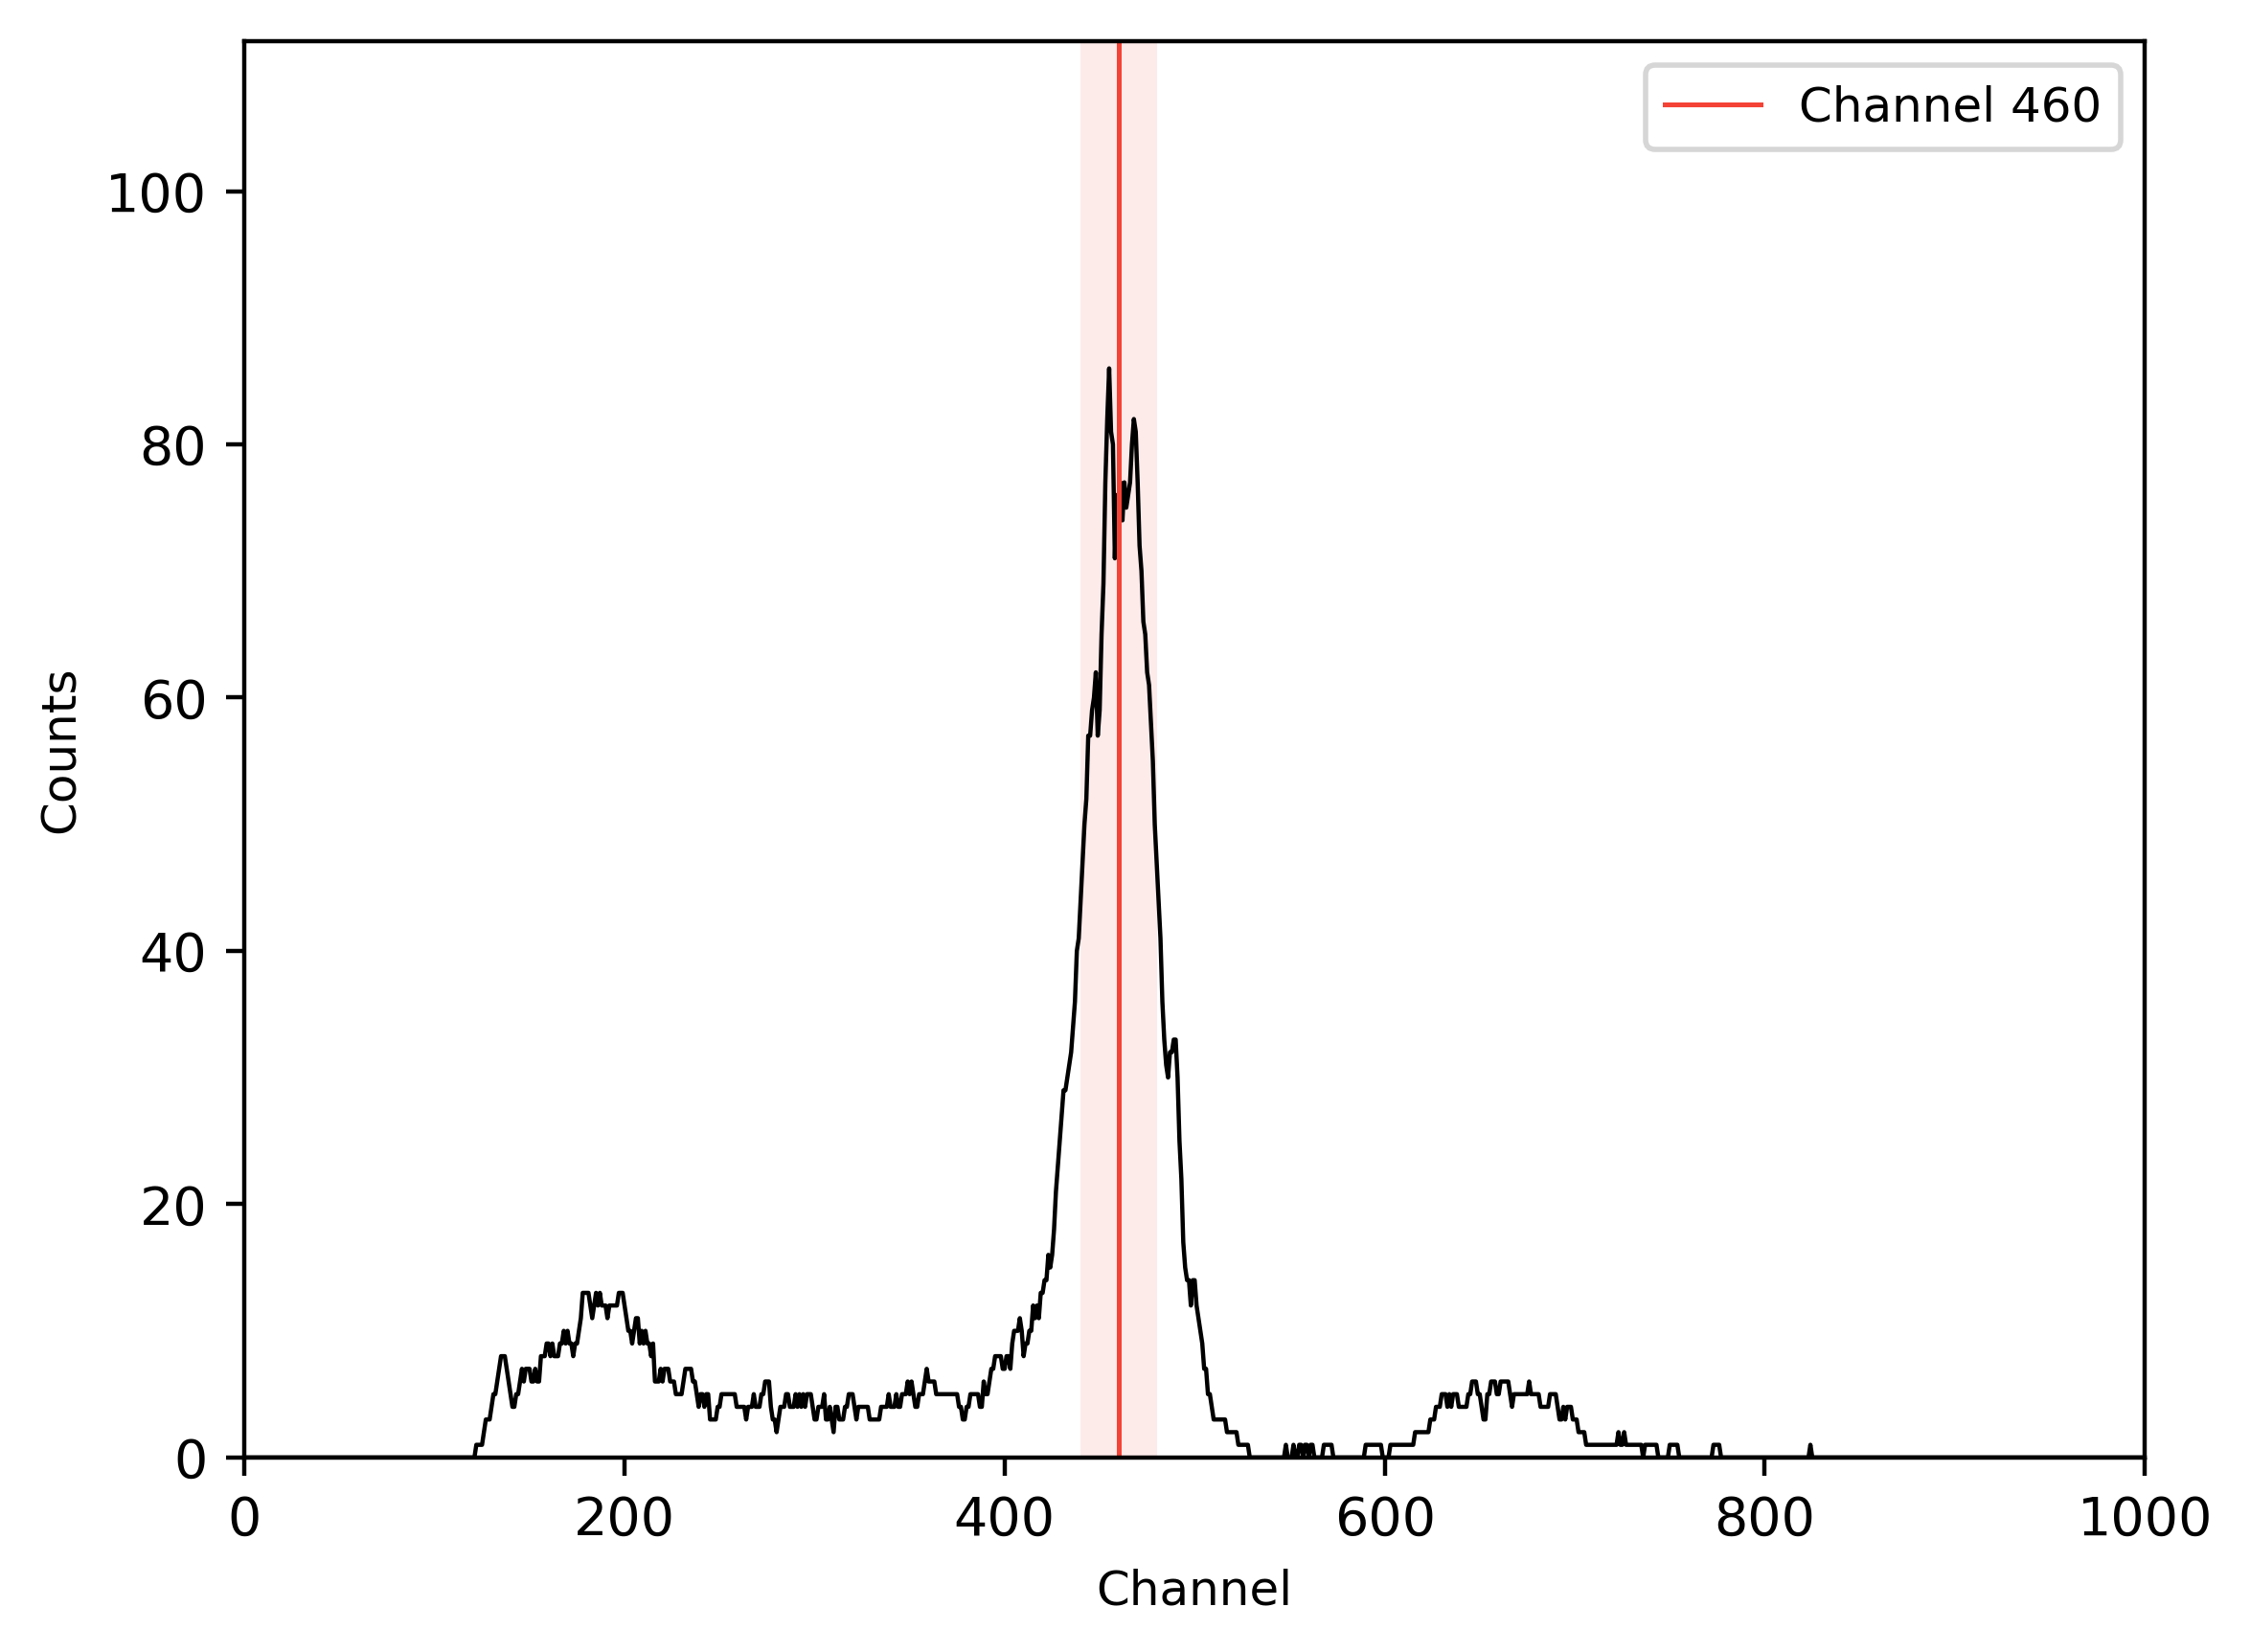
\includegraphics[]{png/comptonpeak}
    \end{adjustbox}
    \captionof{figure}{comptonpeak}
    \label{fig:}
\end{center}
%
\begin{center}
    \begin{adjustbox}{max width=\linewidth, keepaspectratio}
        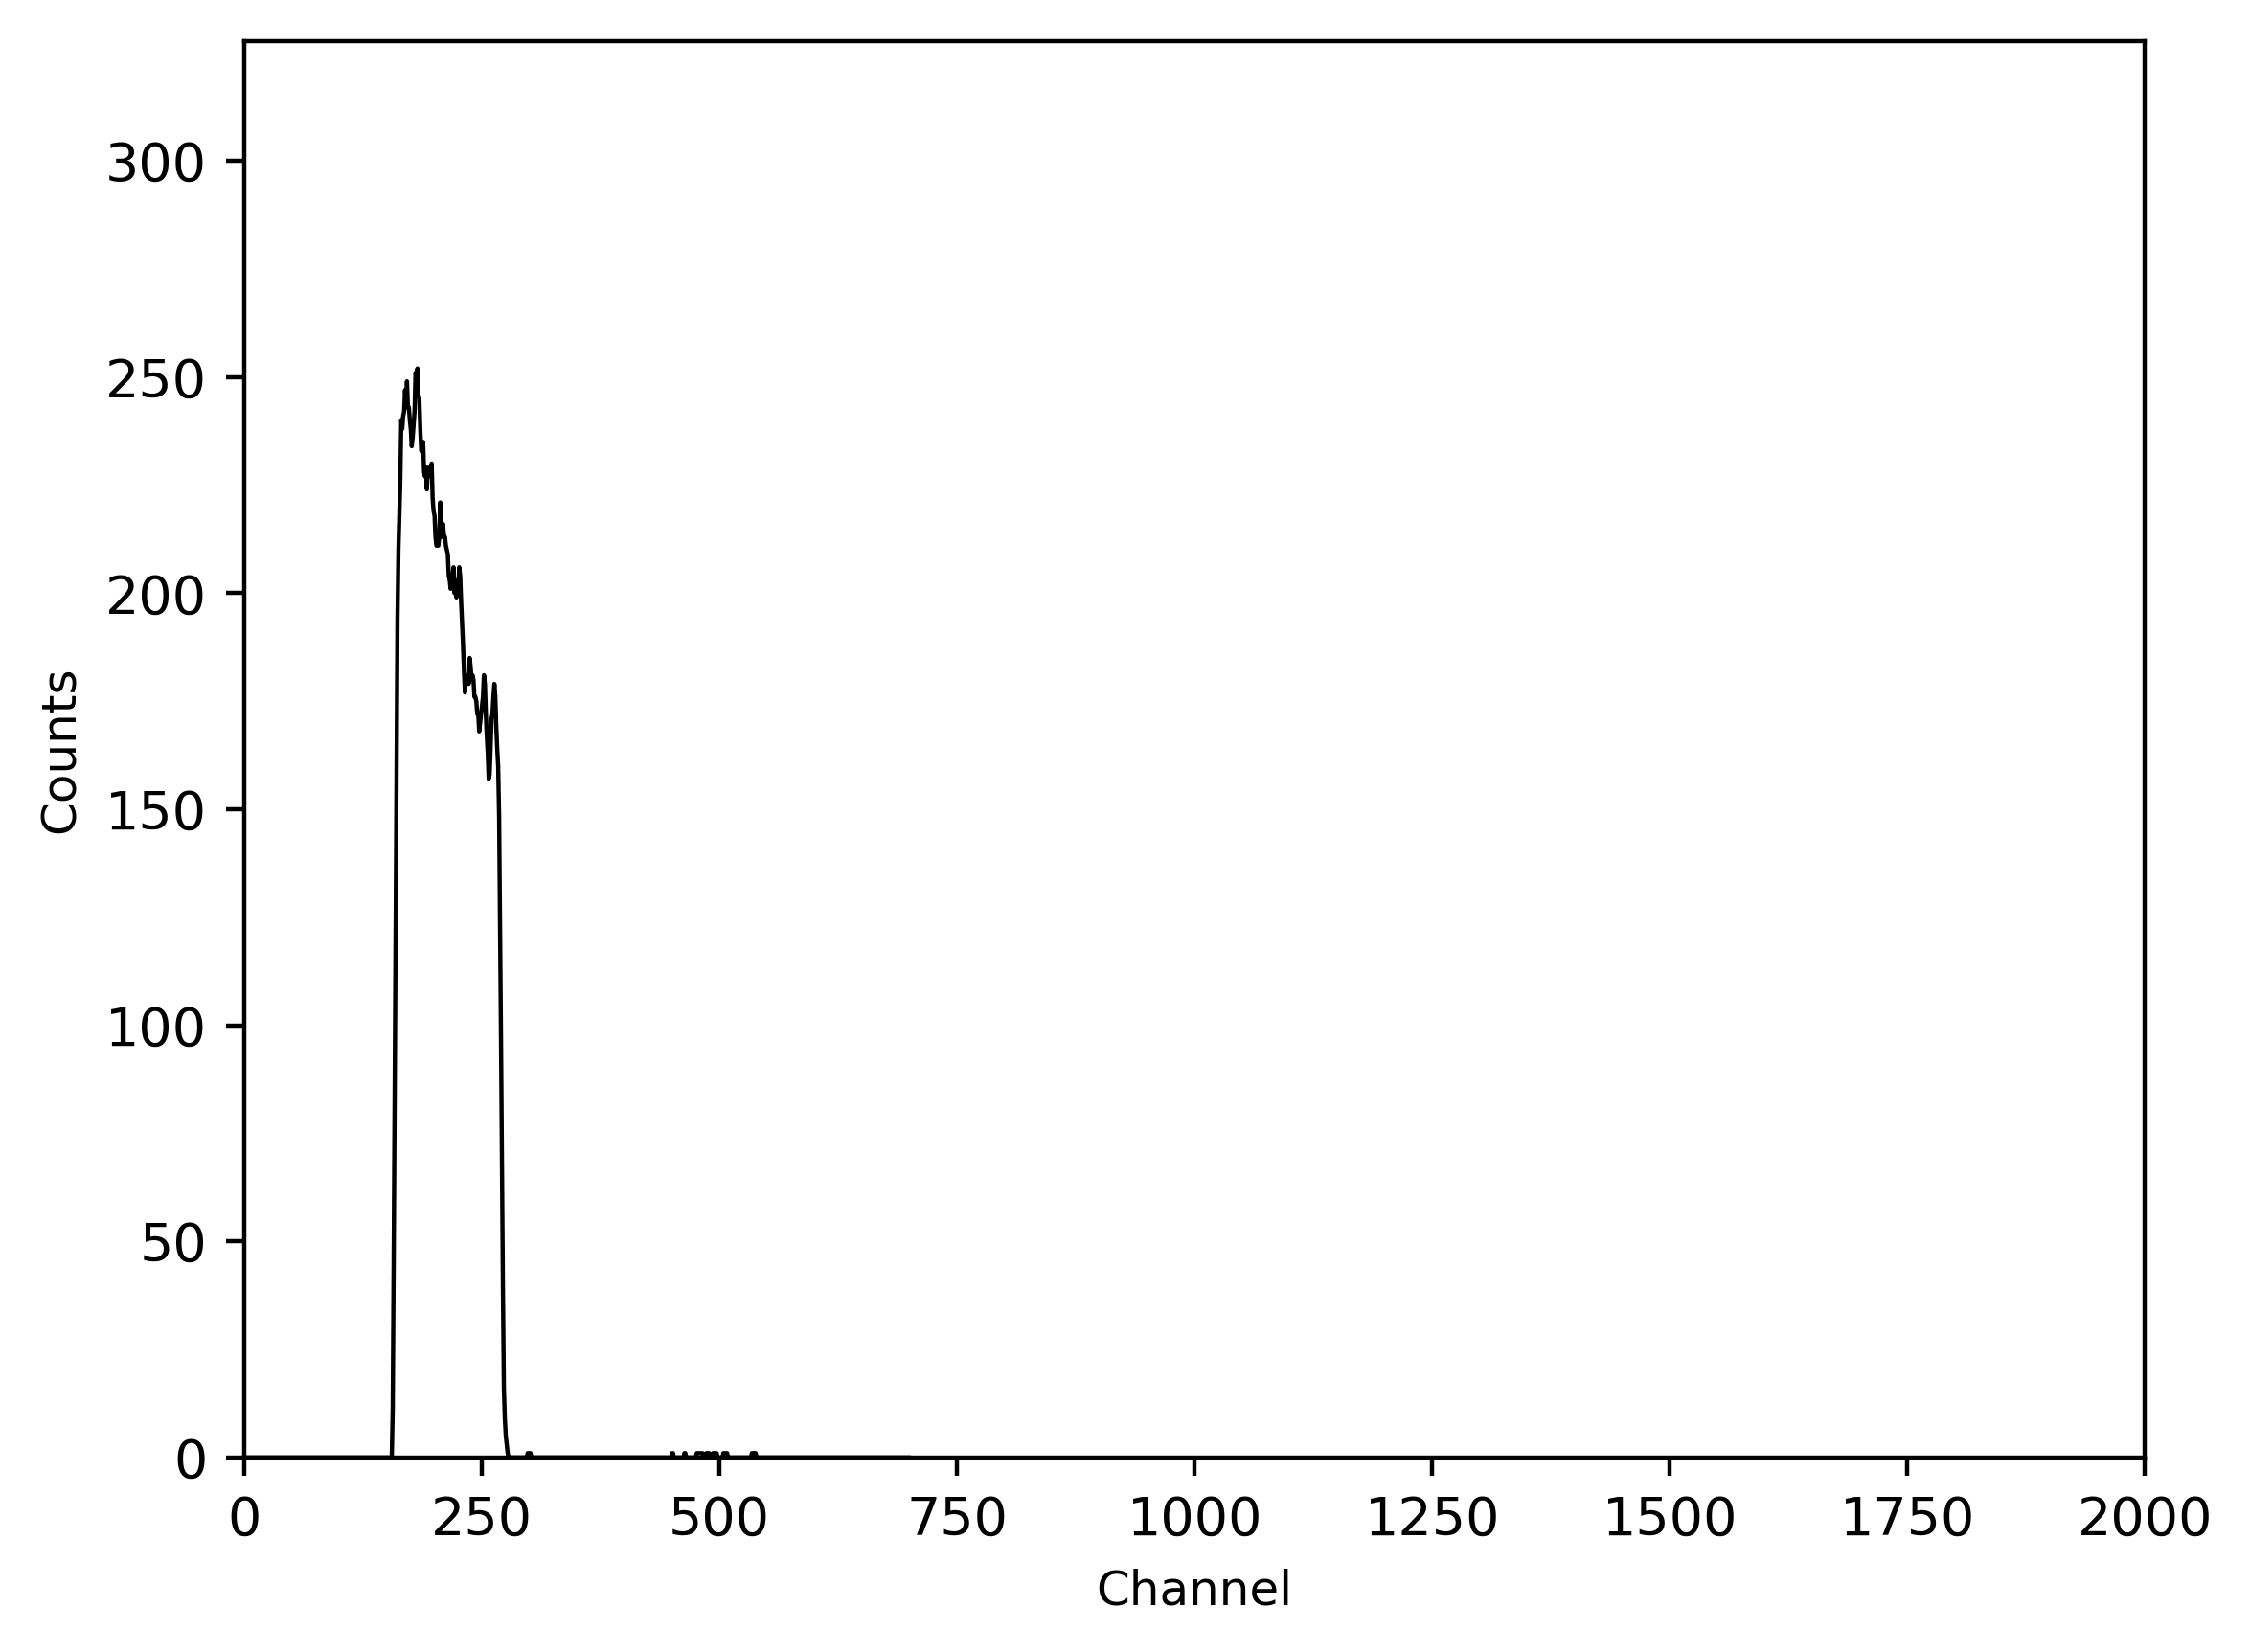
\includegraphics[]{png/signal2eneriewindow}
    \end{adjustbox}
    \captionof{figure}{signal2eneriewindow}
    \label{fig:}
\end{center}
%
\begin{center}
    \begin{adjustbox}{max width=\linewidth, keepaspectratio}
        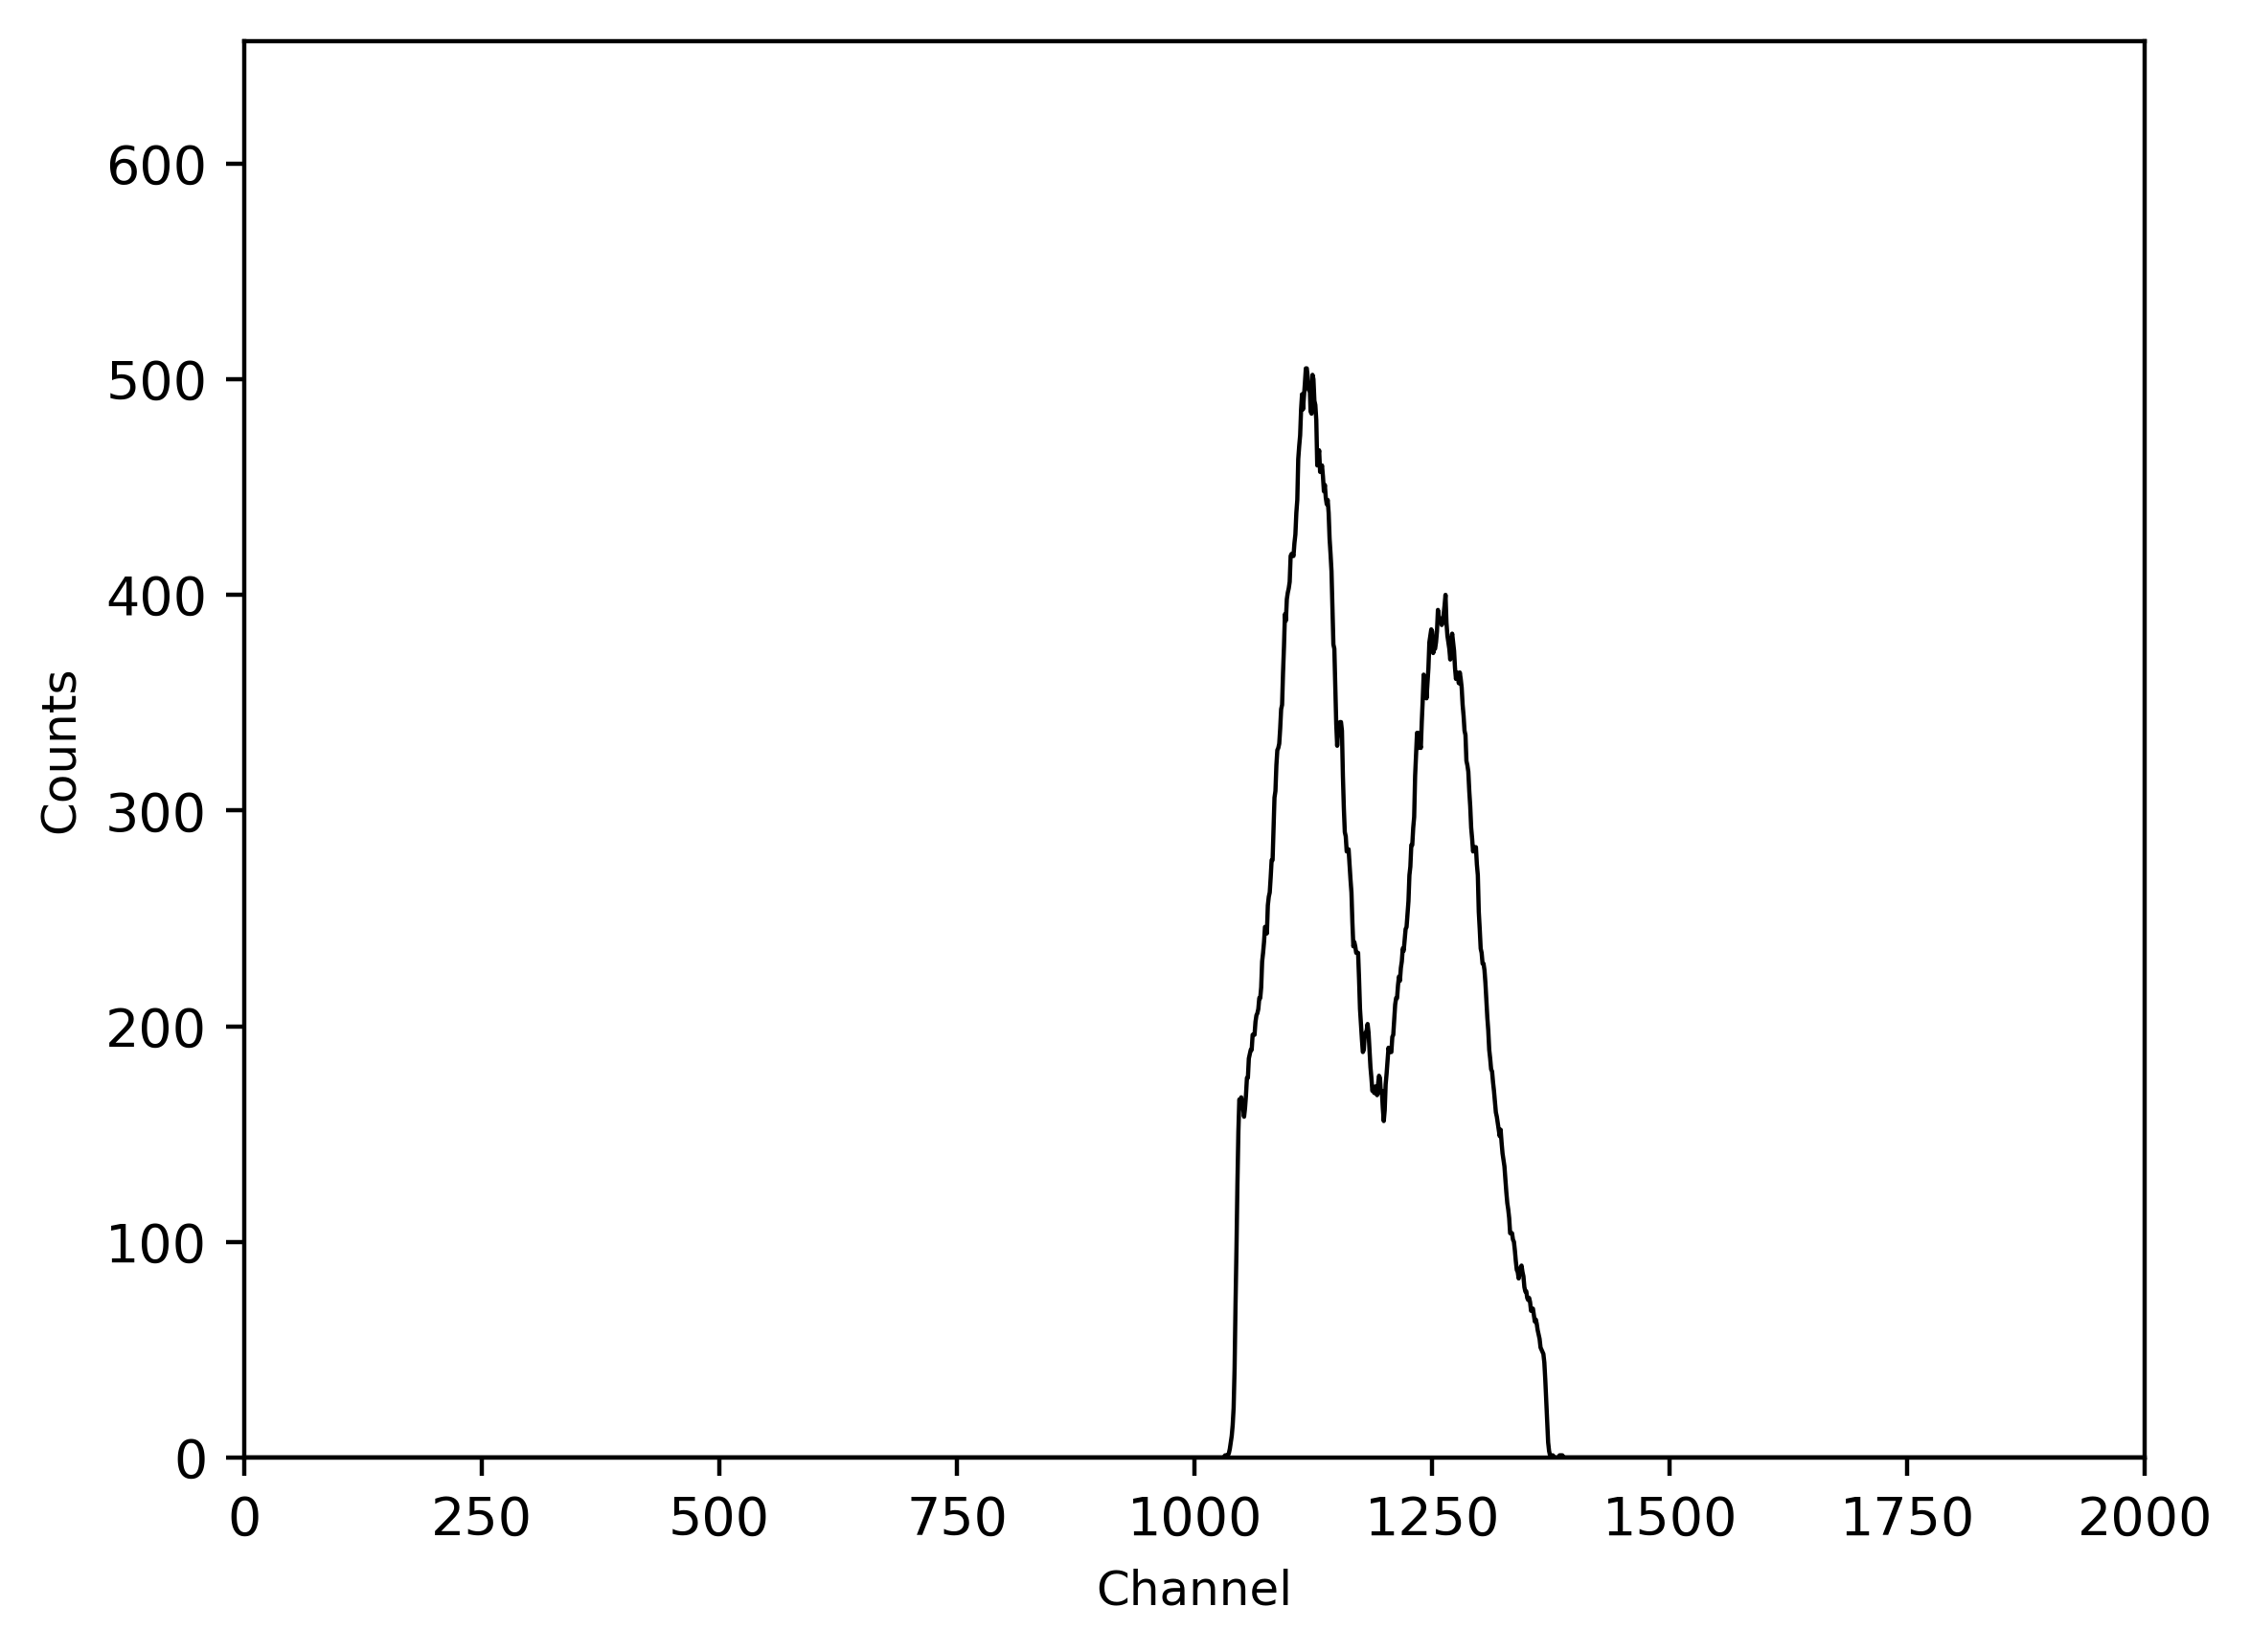
\includegraphics[]{png/60CoEnergiewindow1}
    \end{adjustbox}
    \captionof{figure}{60CoEnergiewindow1}
    \label{fig:}
\end{center}
%
\begin{center}
    \begin{adjustbox}{max width=\linewidth, keepaspectratio}
        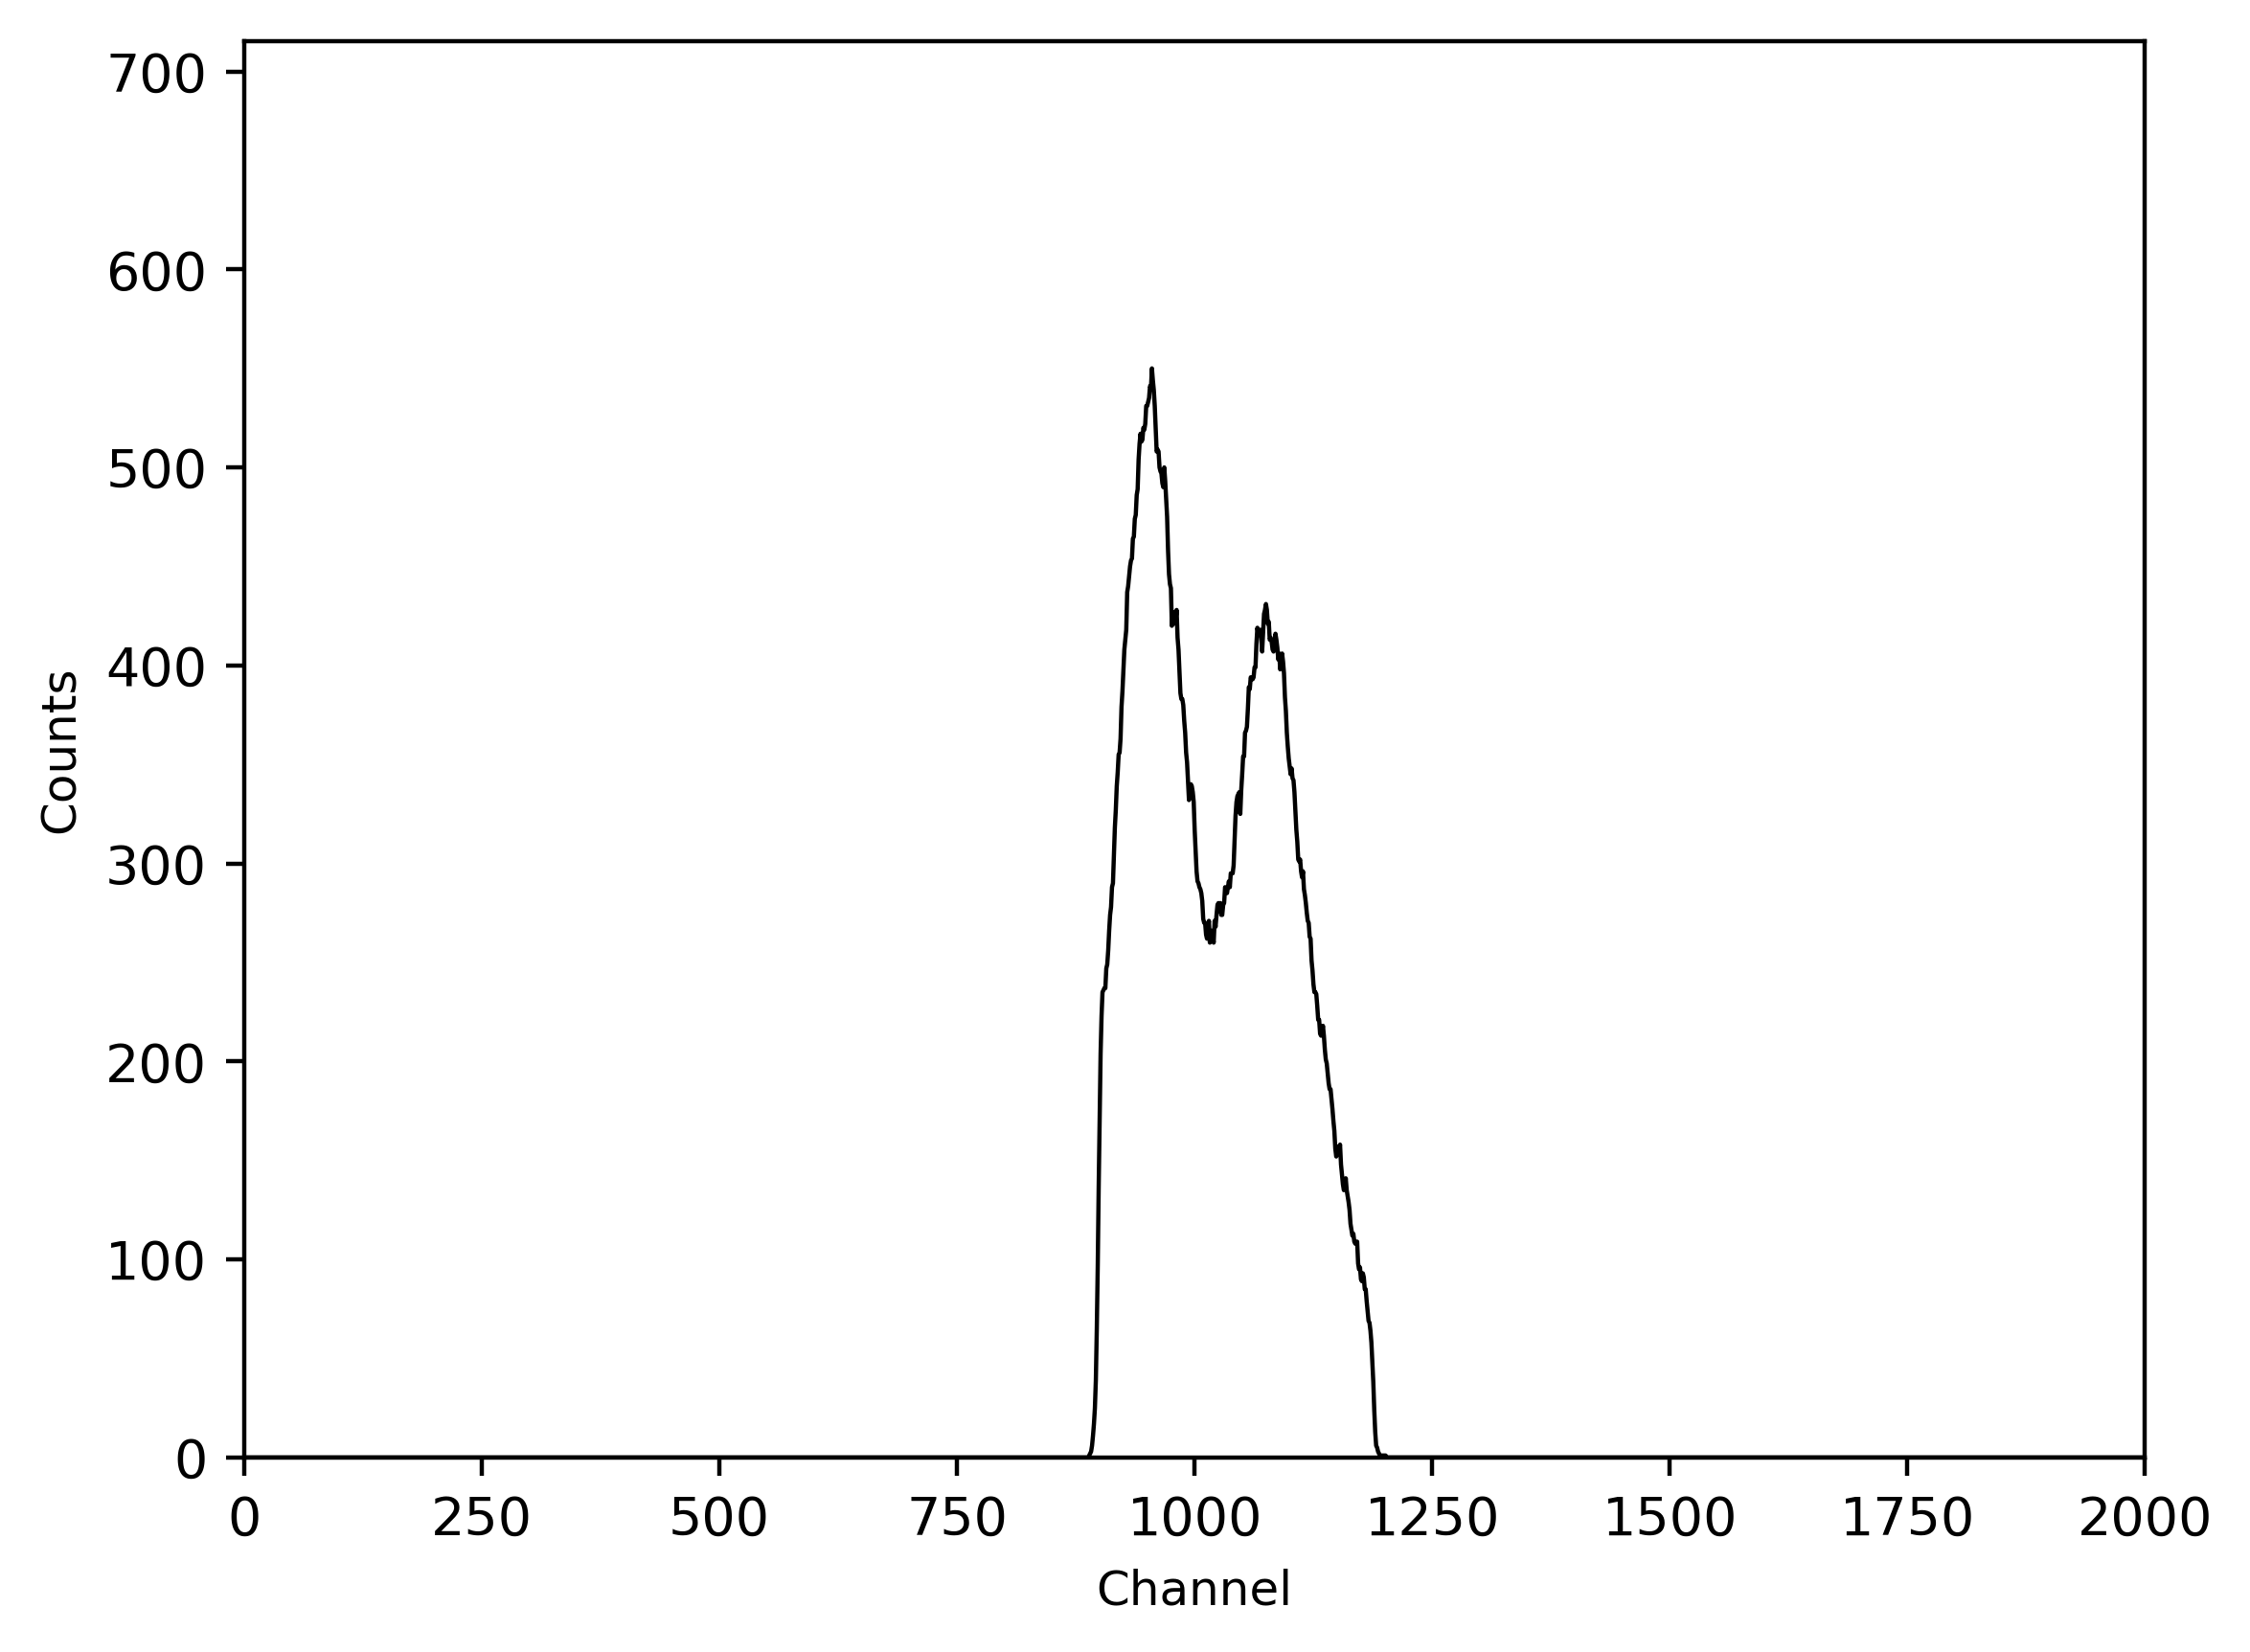
\includegraphics[]{png/60CoEnergiewindow2}
    \end{adjustbox}
    \captionof{figure}{60CoEnergiewindow2}
    \label{fig:}
\end{center}
%
\begin{center}
    \begin{adjustbox}{max width=\linewidth, keepaspectratio}
        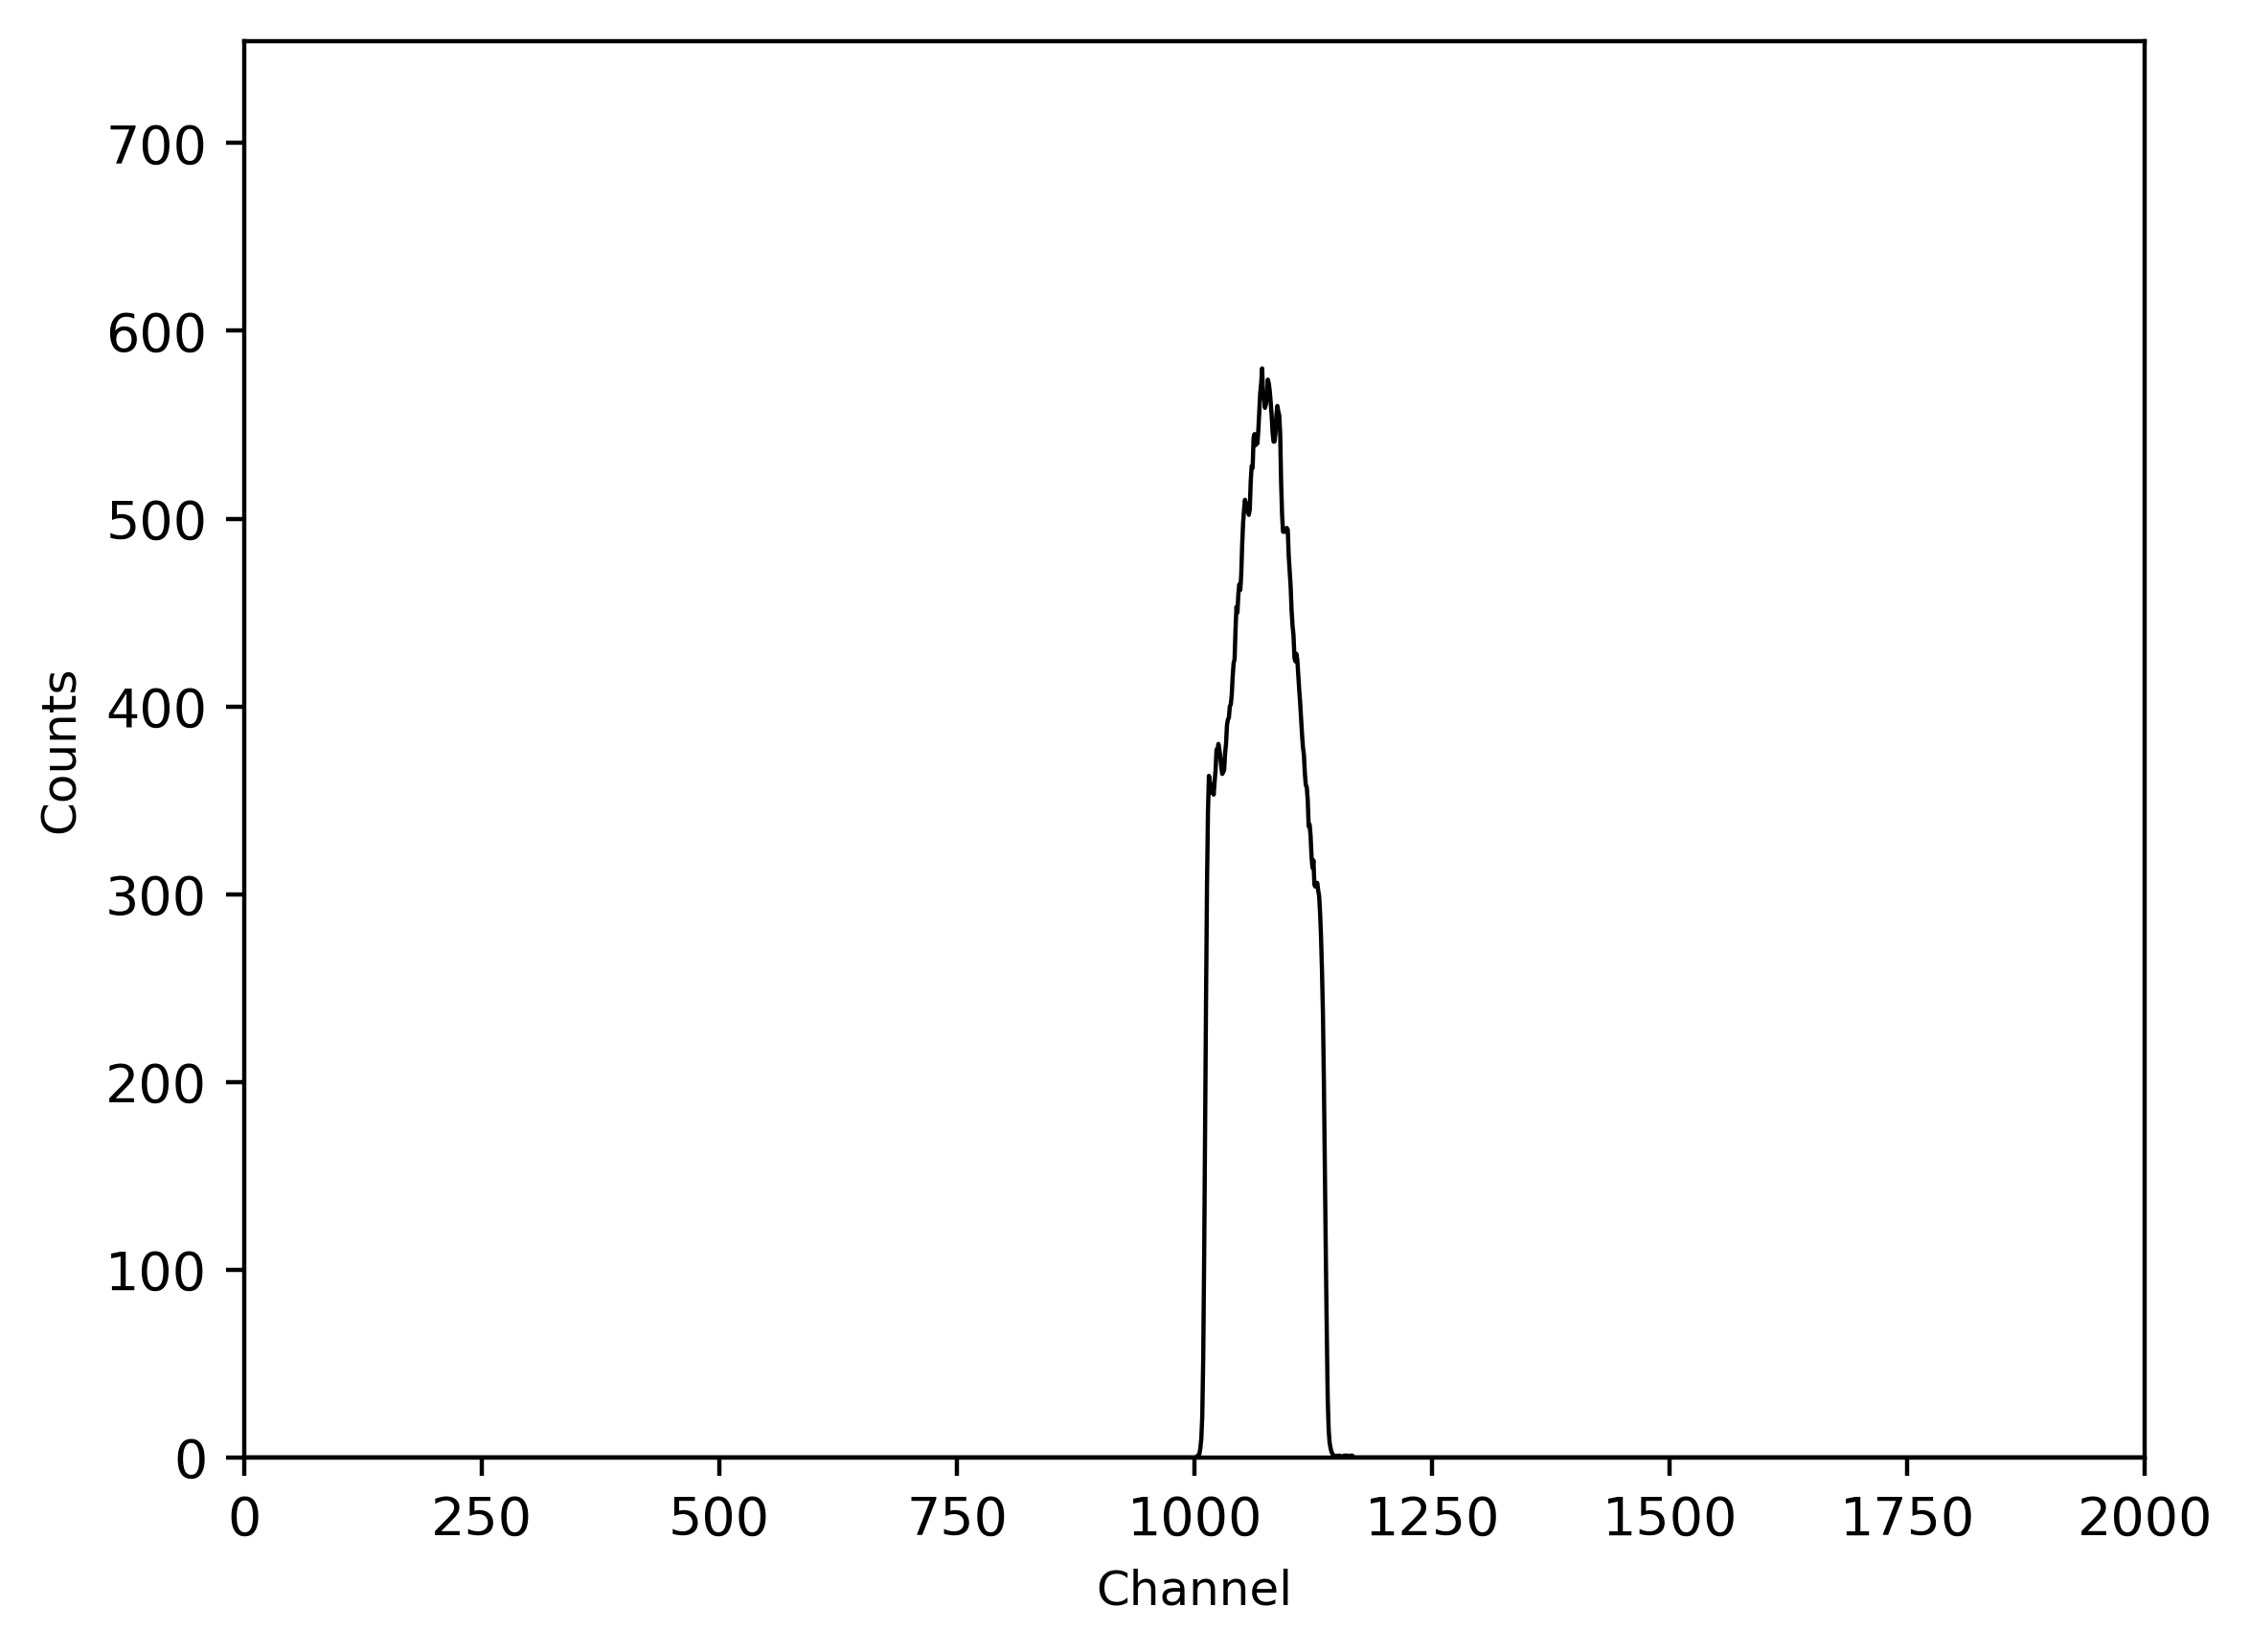
\includegraphics[]{png/60CoEnergiewindow2-peak2}
    \end{adjustbox}
    \captionof{figure}{60CoEnergiewindow2-peak2}
    \label{fig:}
\end{center}
%
\begin{center}
    \begin{adjustbox}{max width=\linewidth, keepaspectratio}
        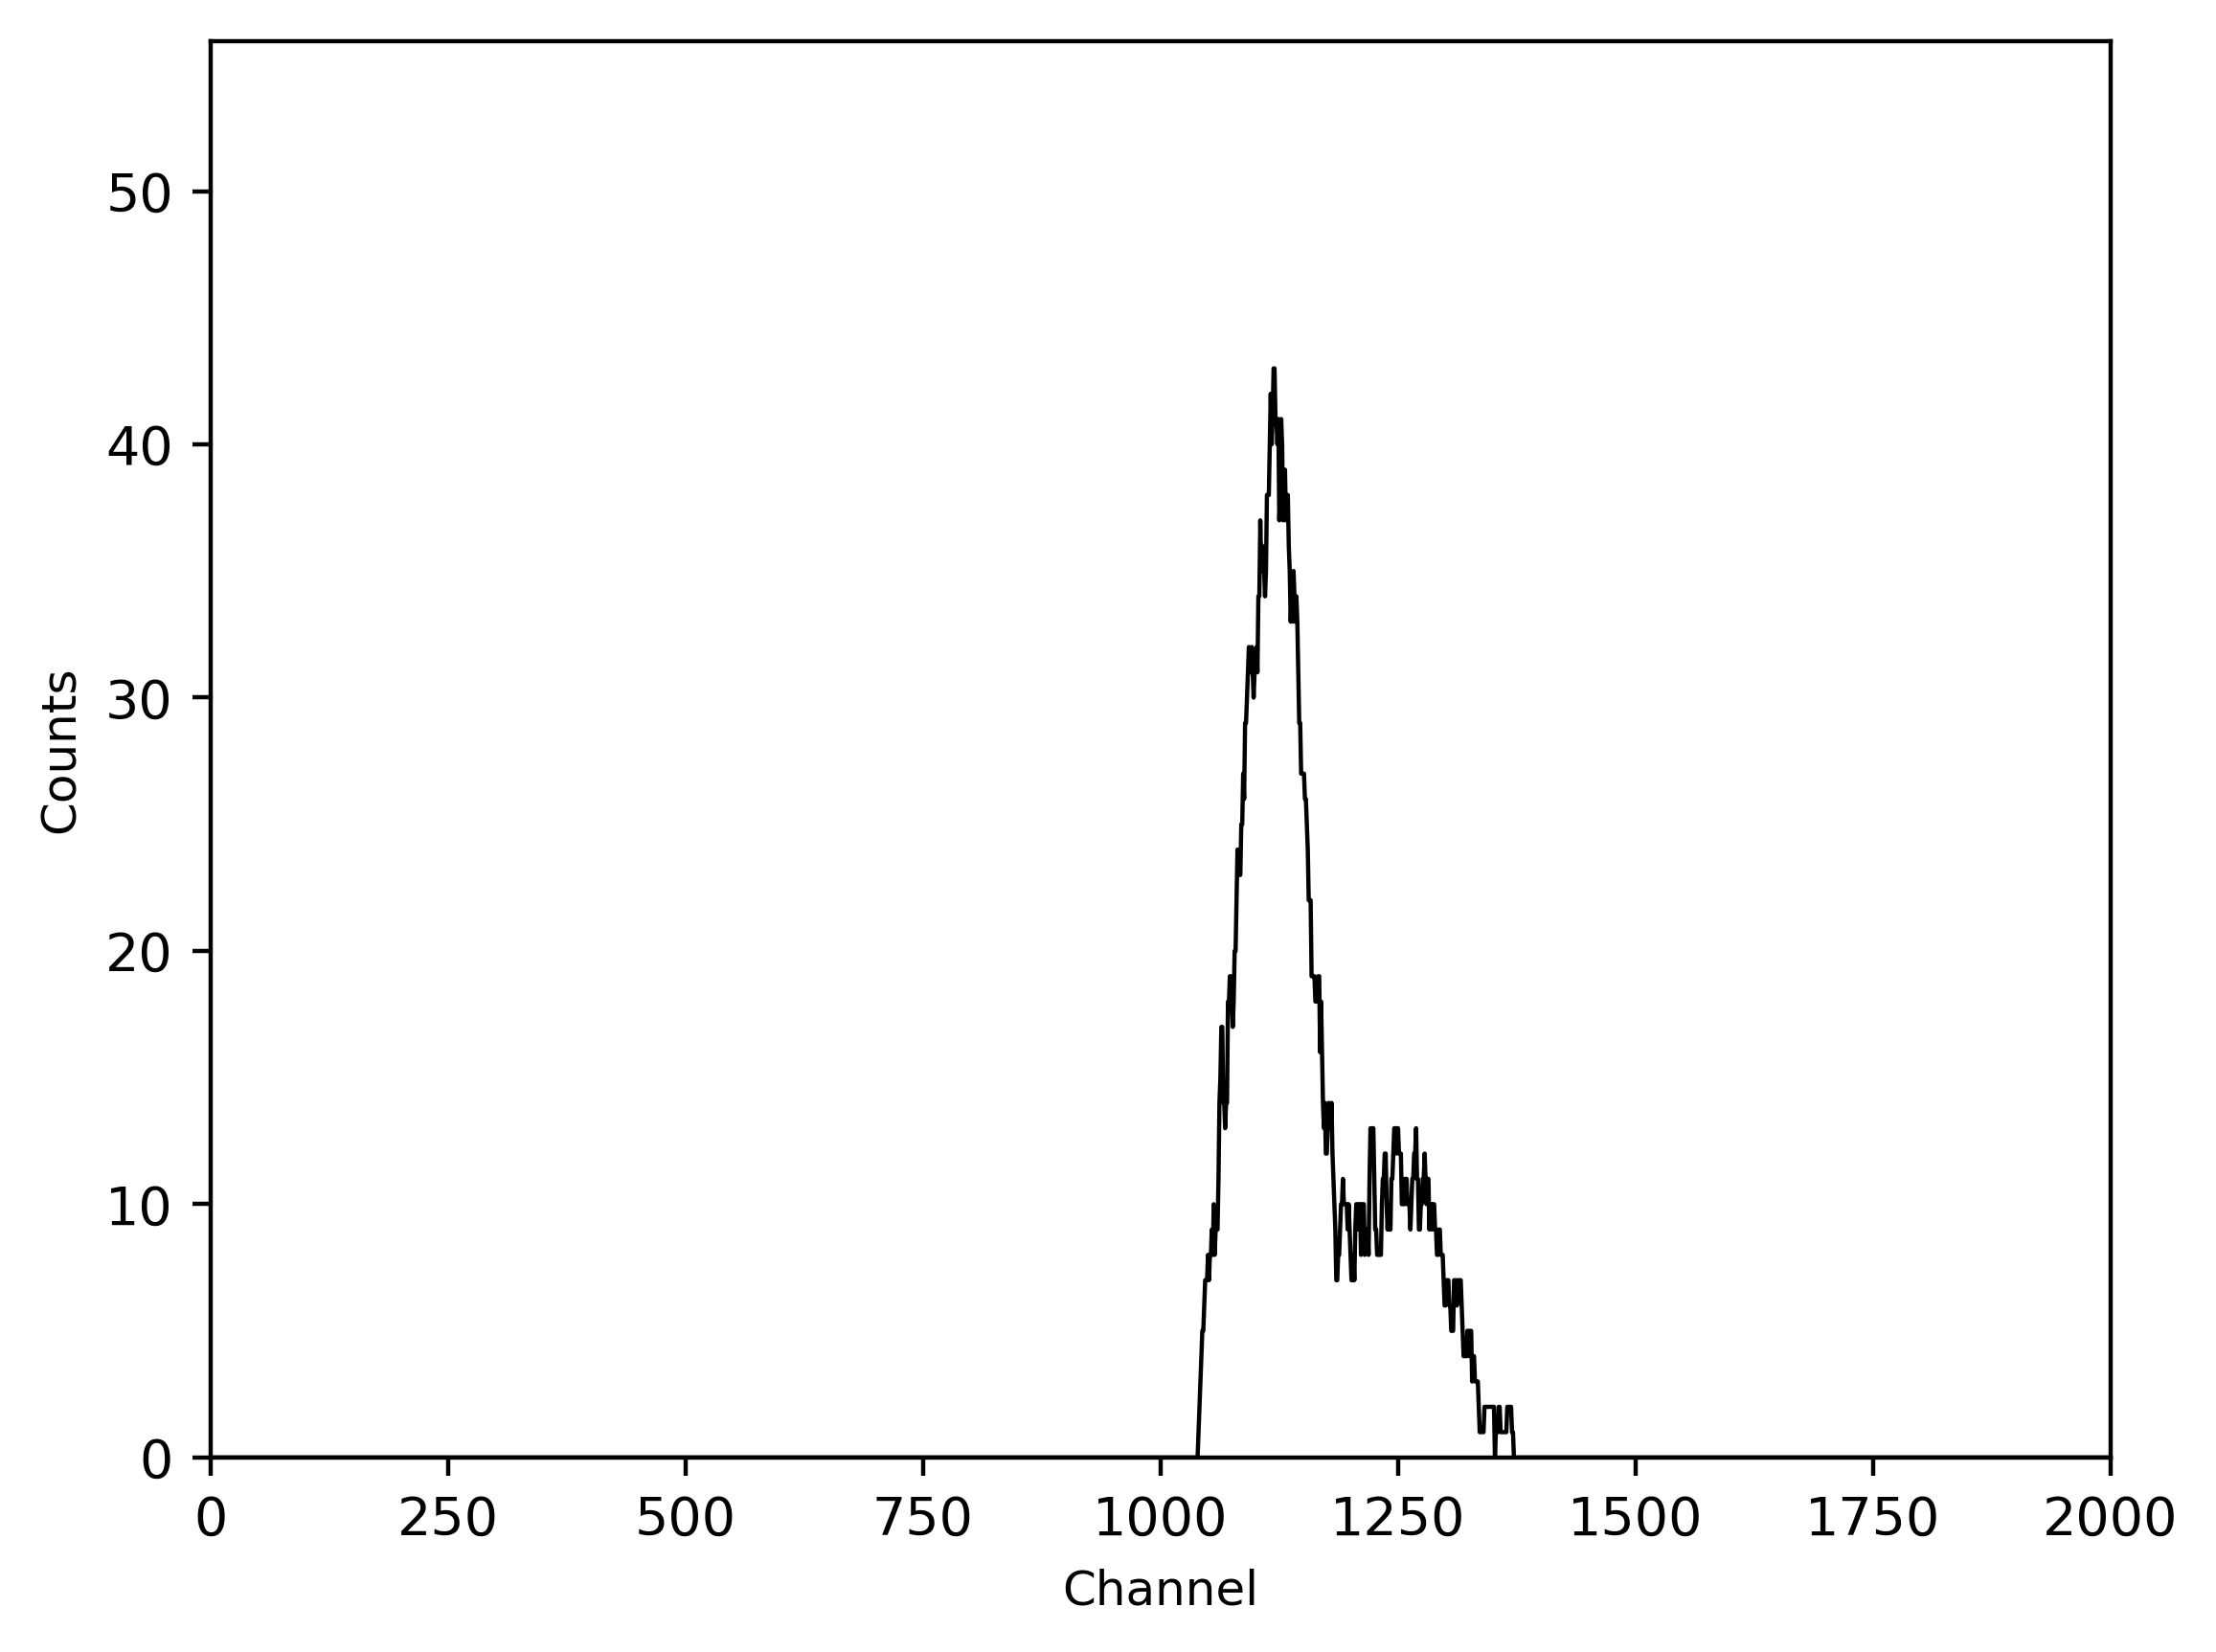
\includegraphics[]{png/60CoKaskadenEnergiewindowBeiPeak2}
    \end{adjustbox}
    \captionof{figure}{60CoKaskadenEnergiewindowBeiPeak2}
    \label{fig:}
\end{center}
%
\begin{center}
    \begin{adjustbox}{max width=\linewidth, keepaspectratio}
        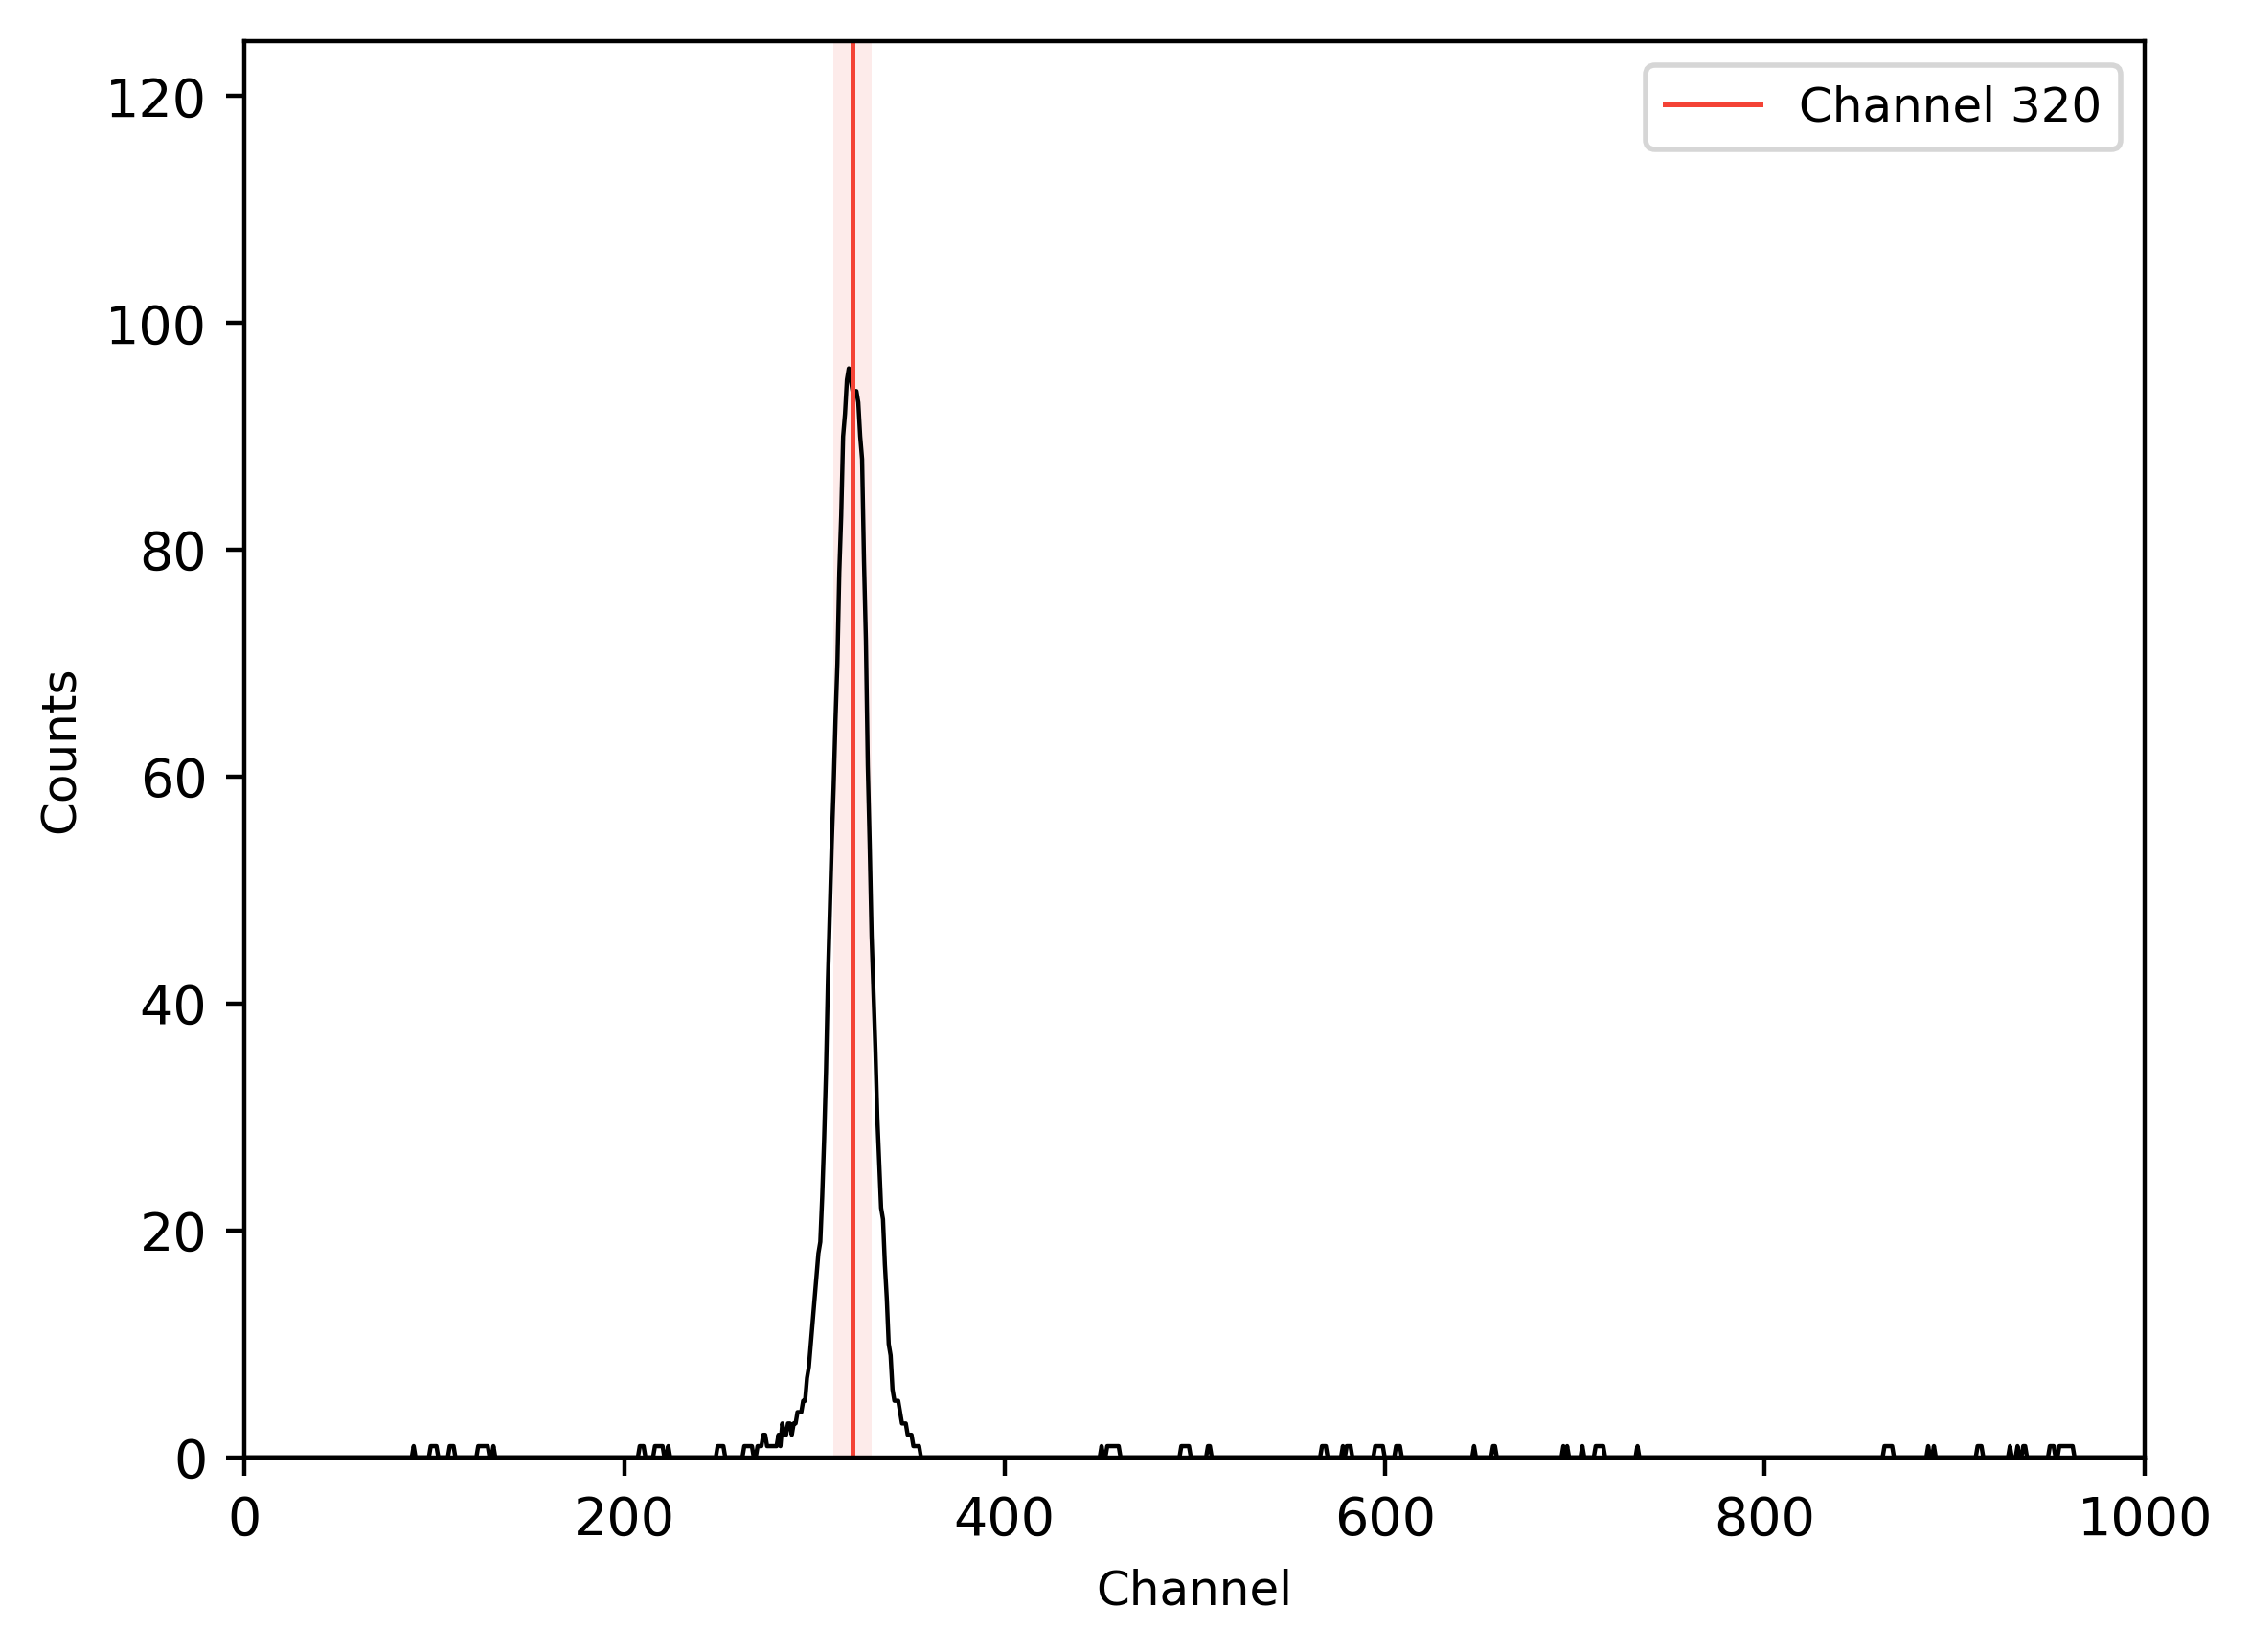
\includegraphics[]{png/60CoZeitspektrum}
    \end{adjustbox}
    \captionof{figure}{60CoZeitspektrum}
    \label{fig:}
\end{center}
%
\begin{center}
    \begin{adjustbox}{max width=\linewidth, keepaspectratio}
        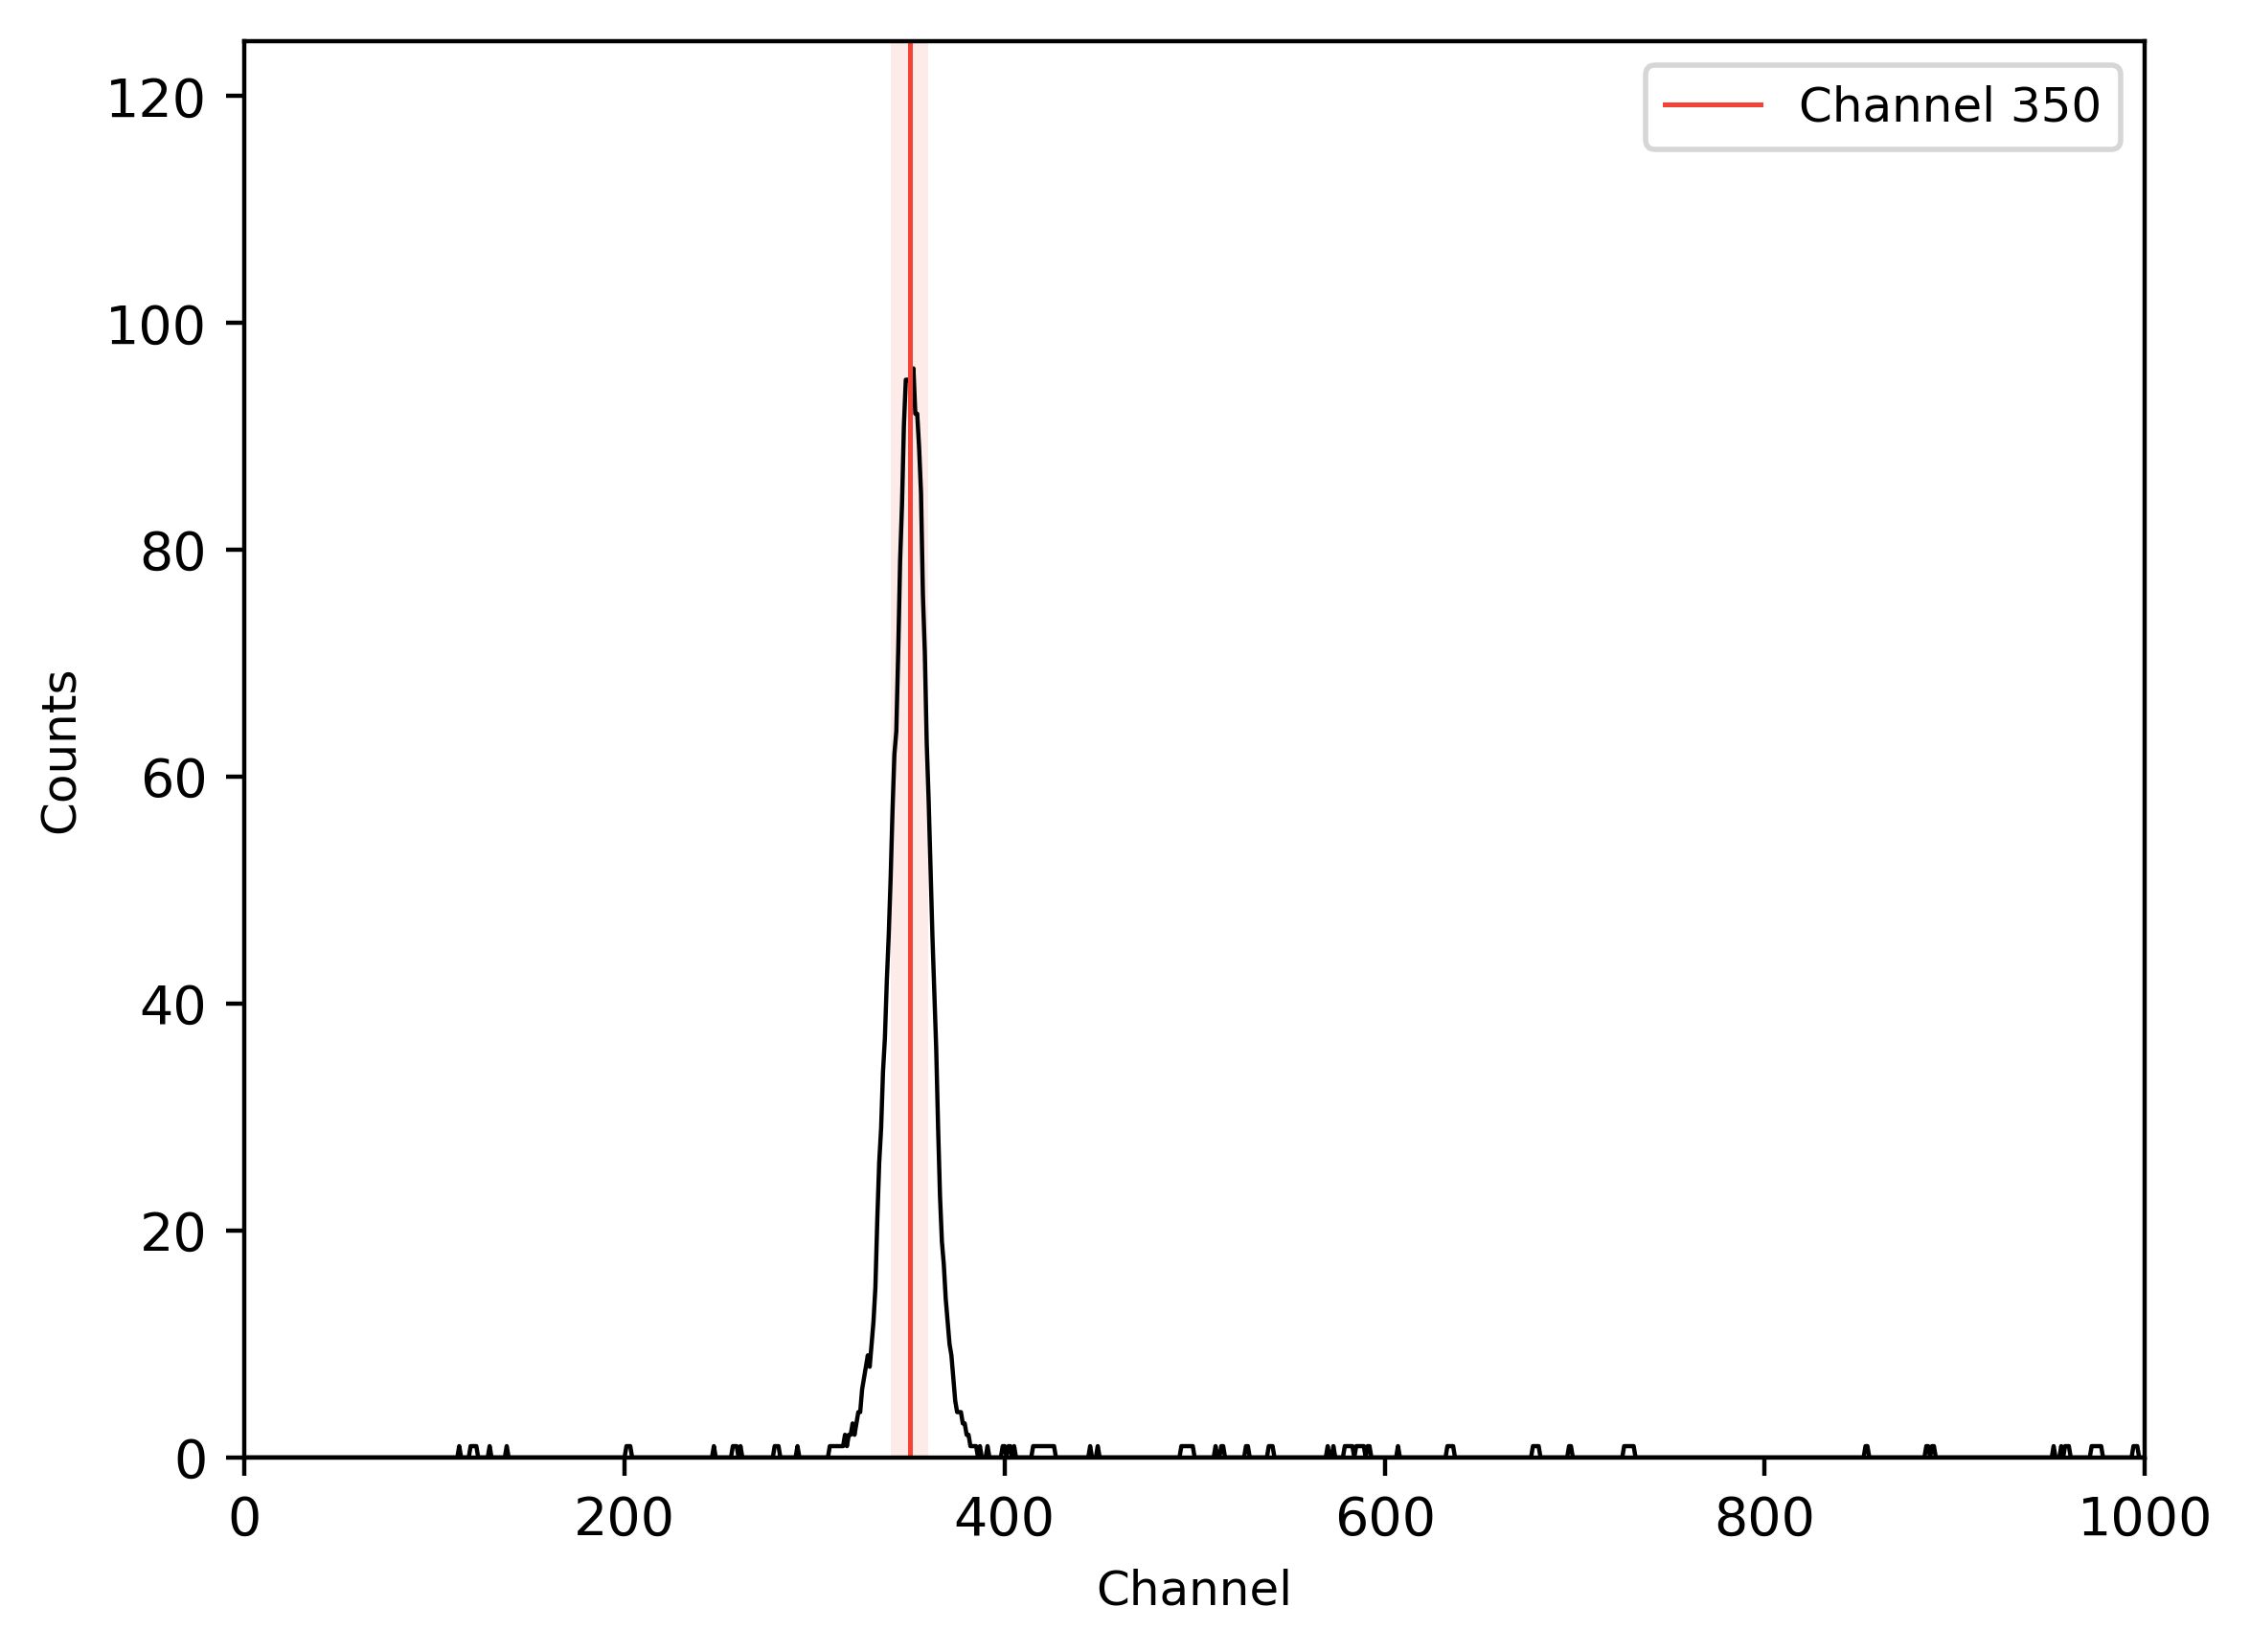
\includegraphics[]{png/60CoZeitspektrum20ns}
    \end{adjustbox}
    \captionof{figure}{60CoZeitspektrum20ns}
    \label{fig:}
\end{center}
%
\begin{center}
    \begin{adjustbox}{max width=\linewidth, keepaspectratio}
        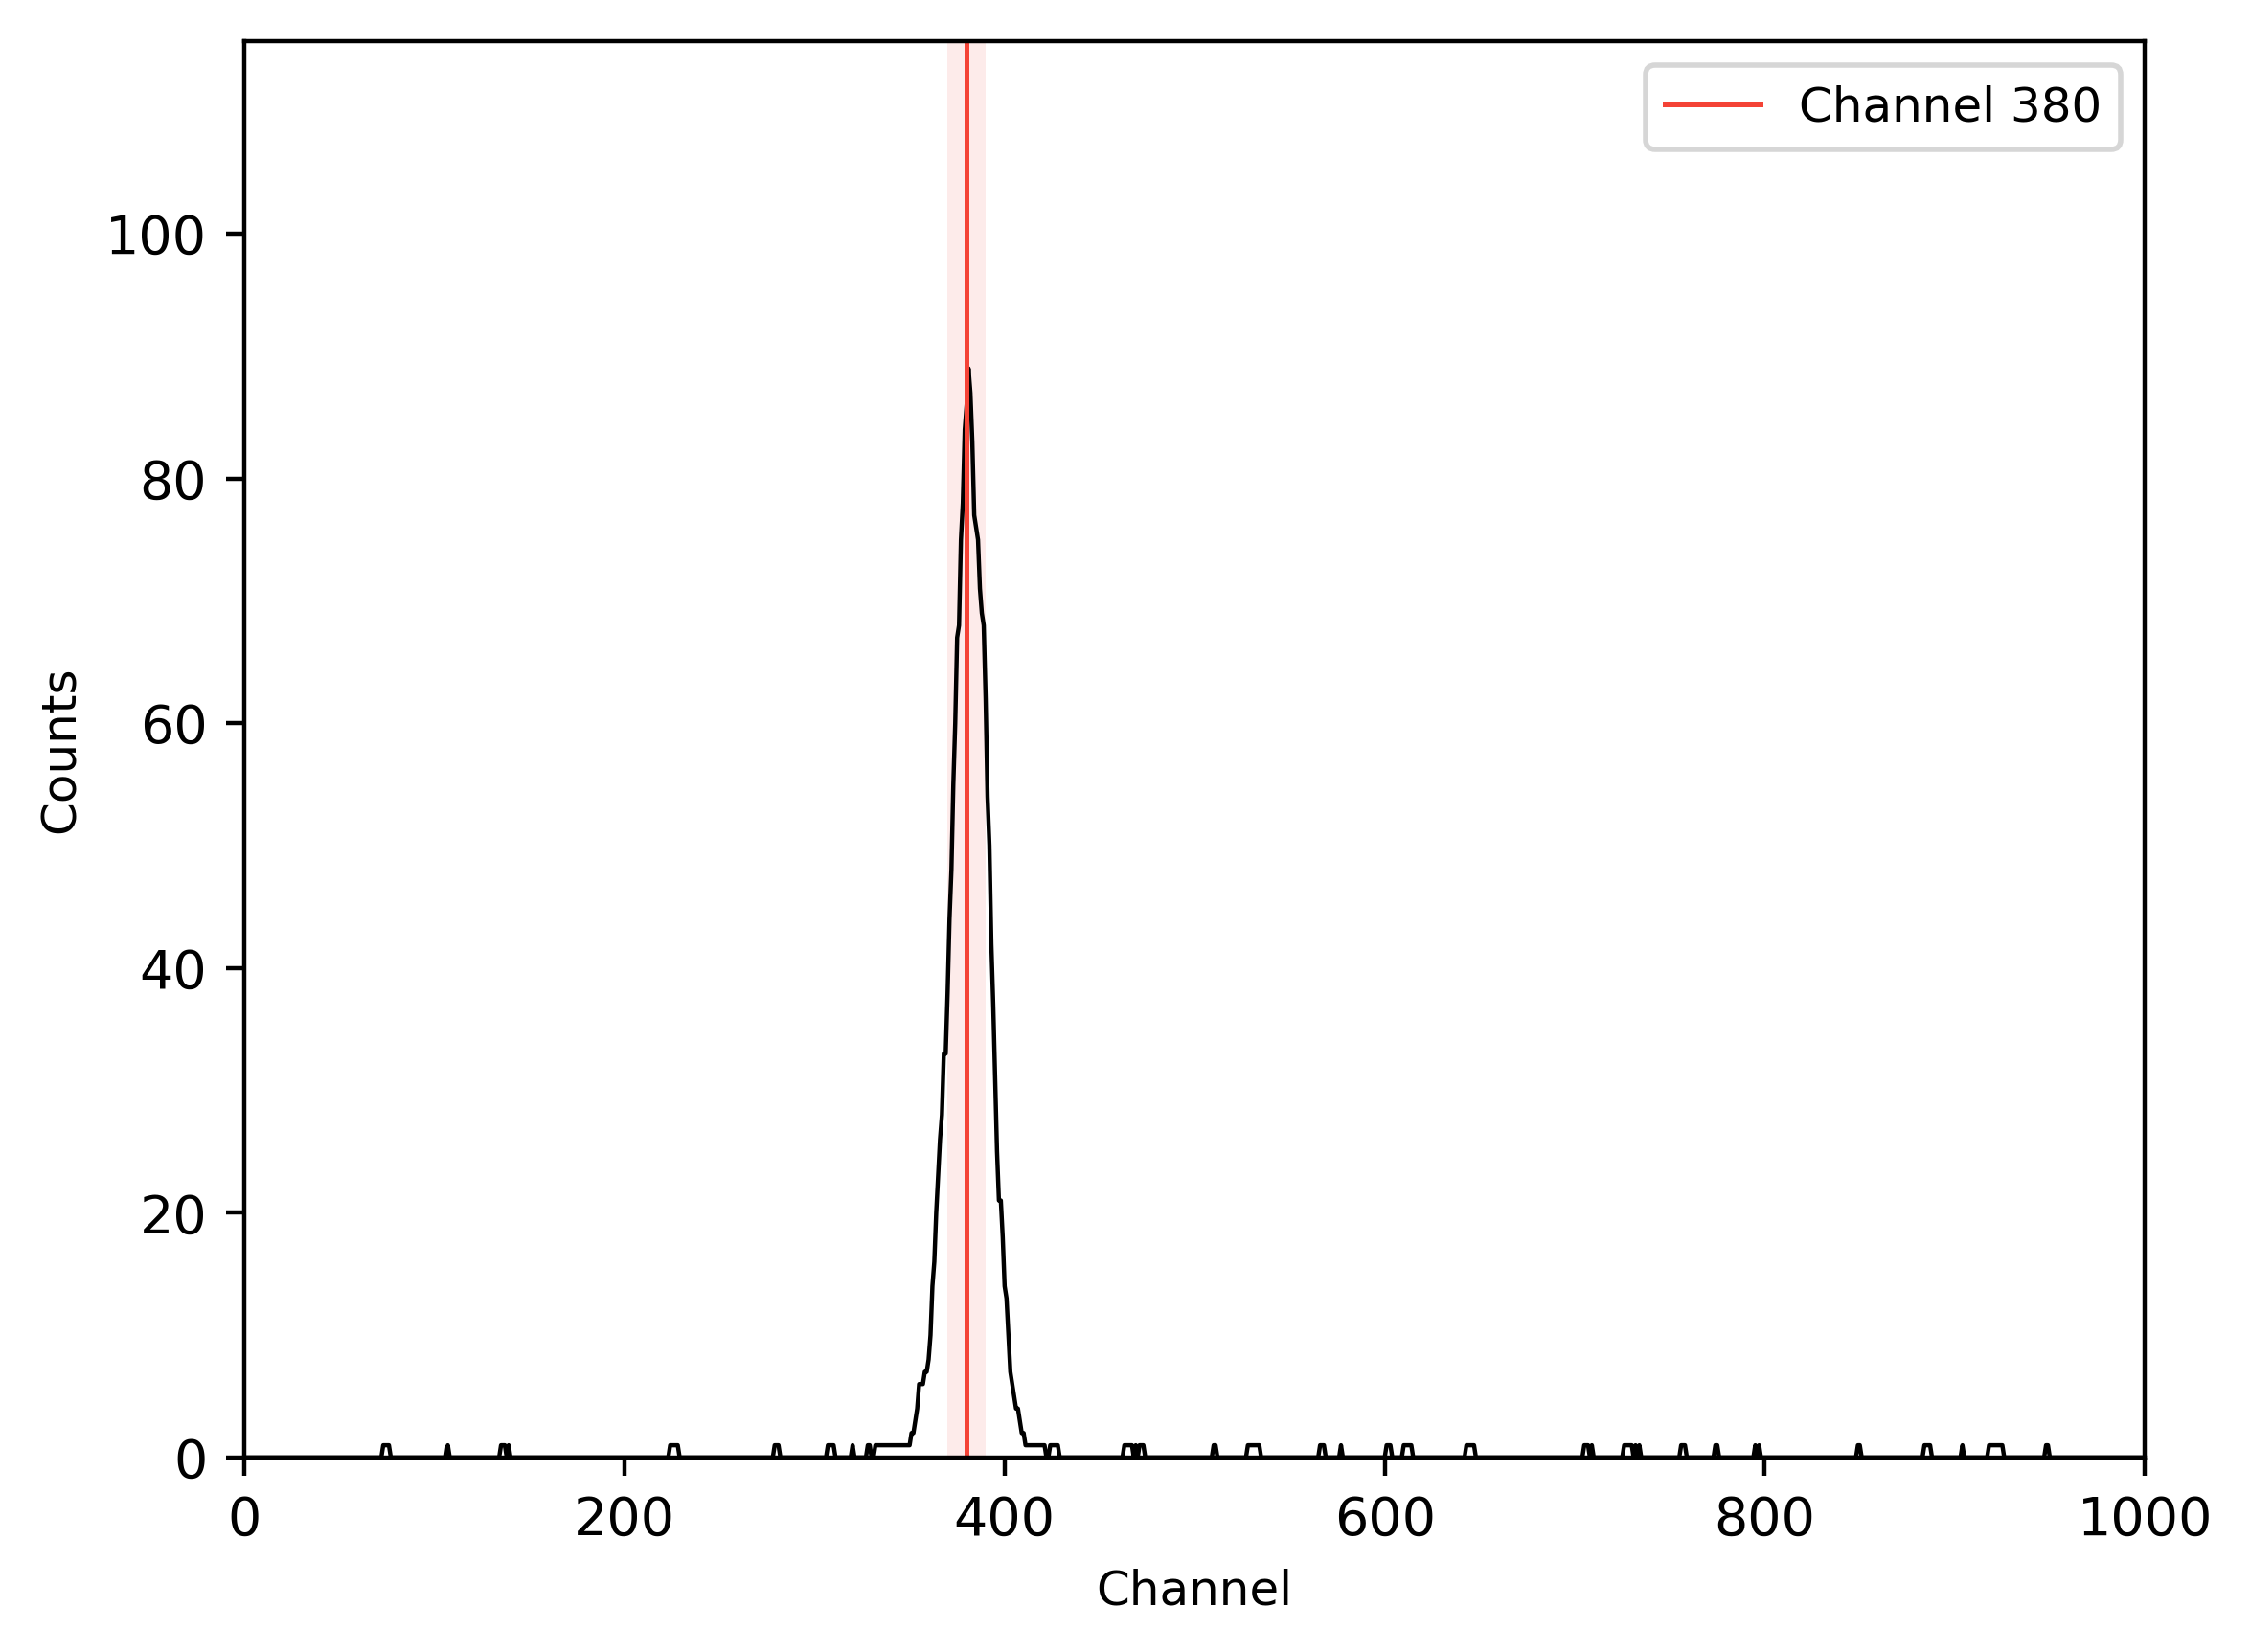
\includegraphics[]{png/60CoZeitspektrum40ns}
    \end{adjustbox}
    \captionof{figure}{60CoZeitspektrum40ns}
    \label{fig:}
\end{center}
%
\begin{center}
    \begin{adjustbox}{max width=\linewidth, keepaspectratio}
        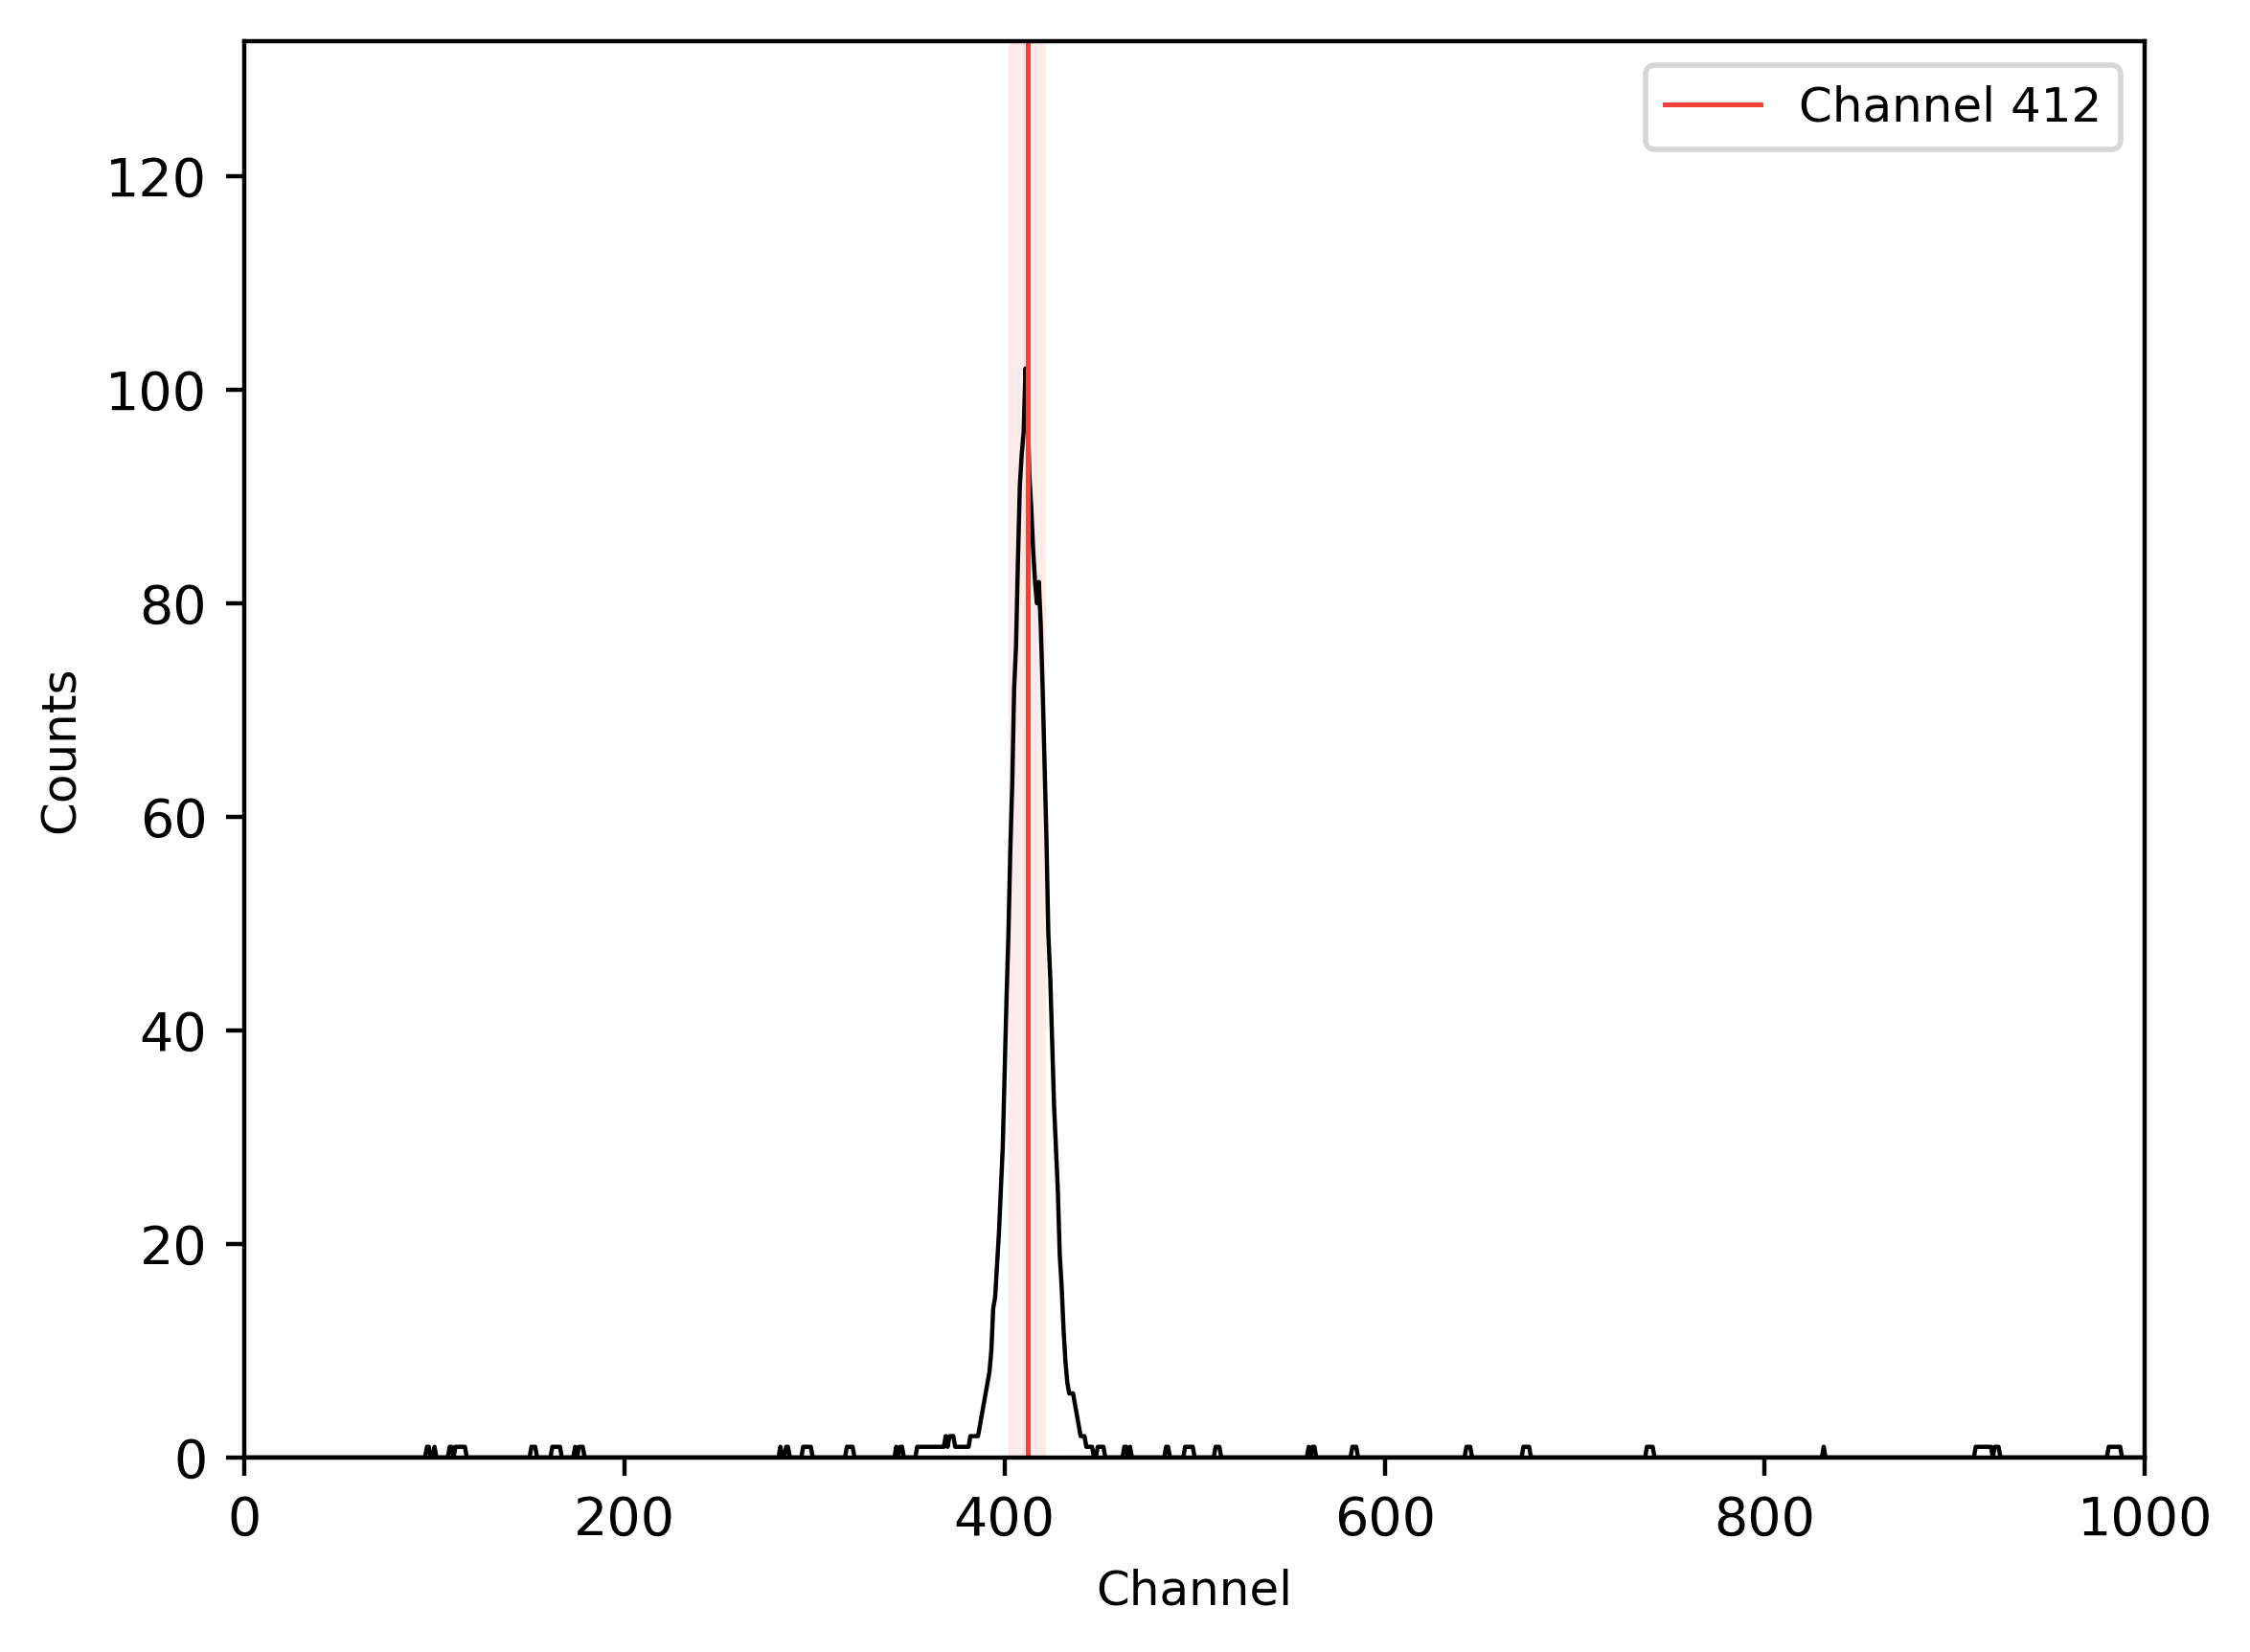
\includegraphics[]{png/60CoZeitspektrum60ns}
    \end{adjustbox}
    \captionof{figure}{60CoZeitspektrum60ns}
    \label{fig:}
\end{center}
%
\begin{center}
    \begin{adjustbox}{max width=\linewidth, keepaspectratio}
        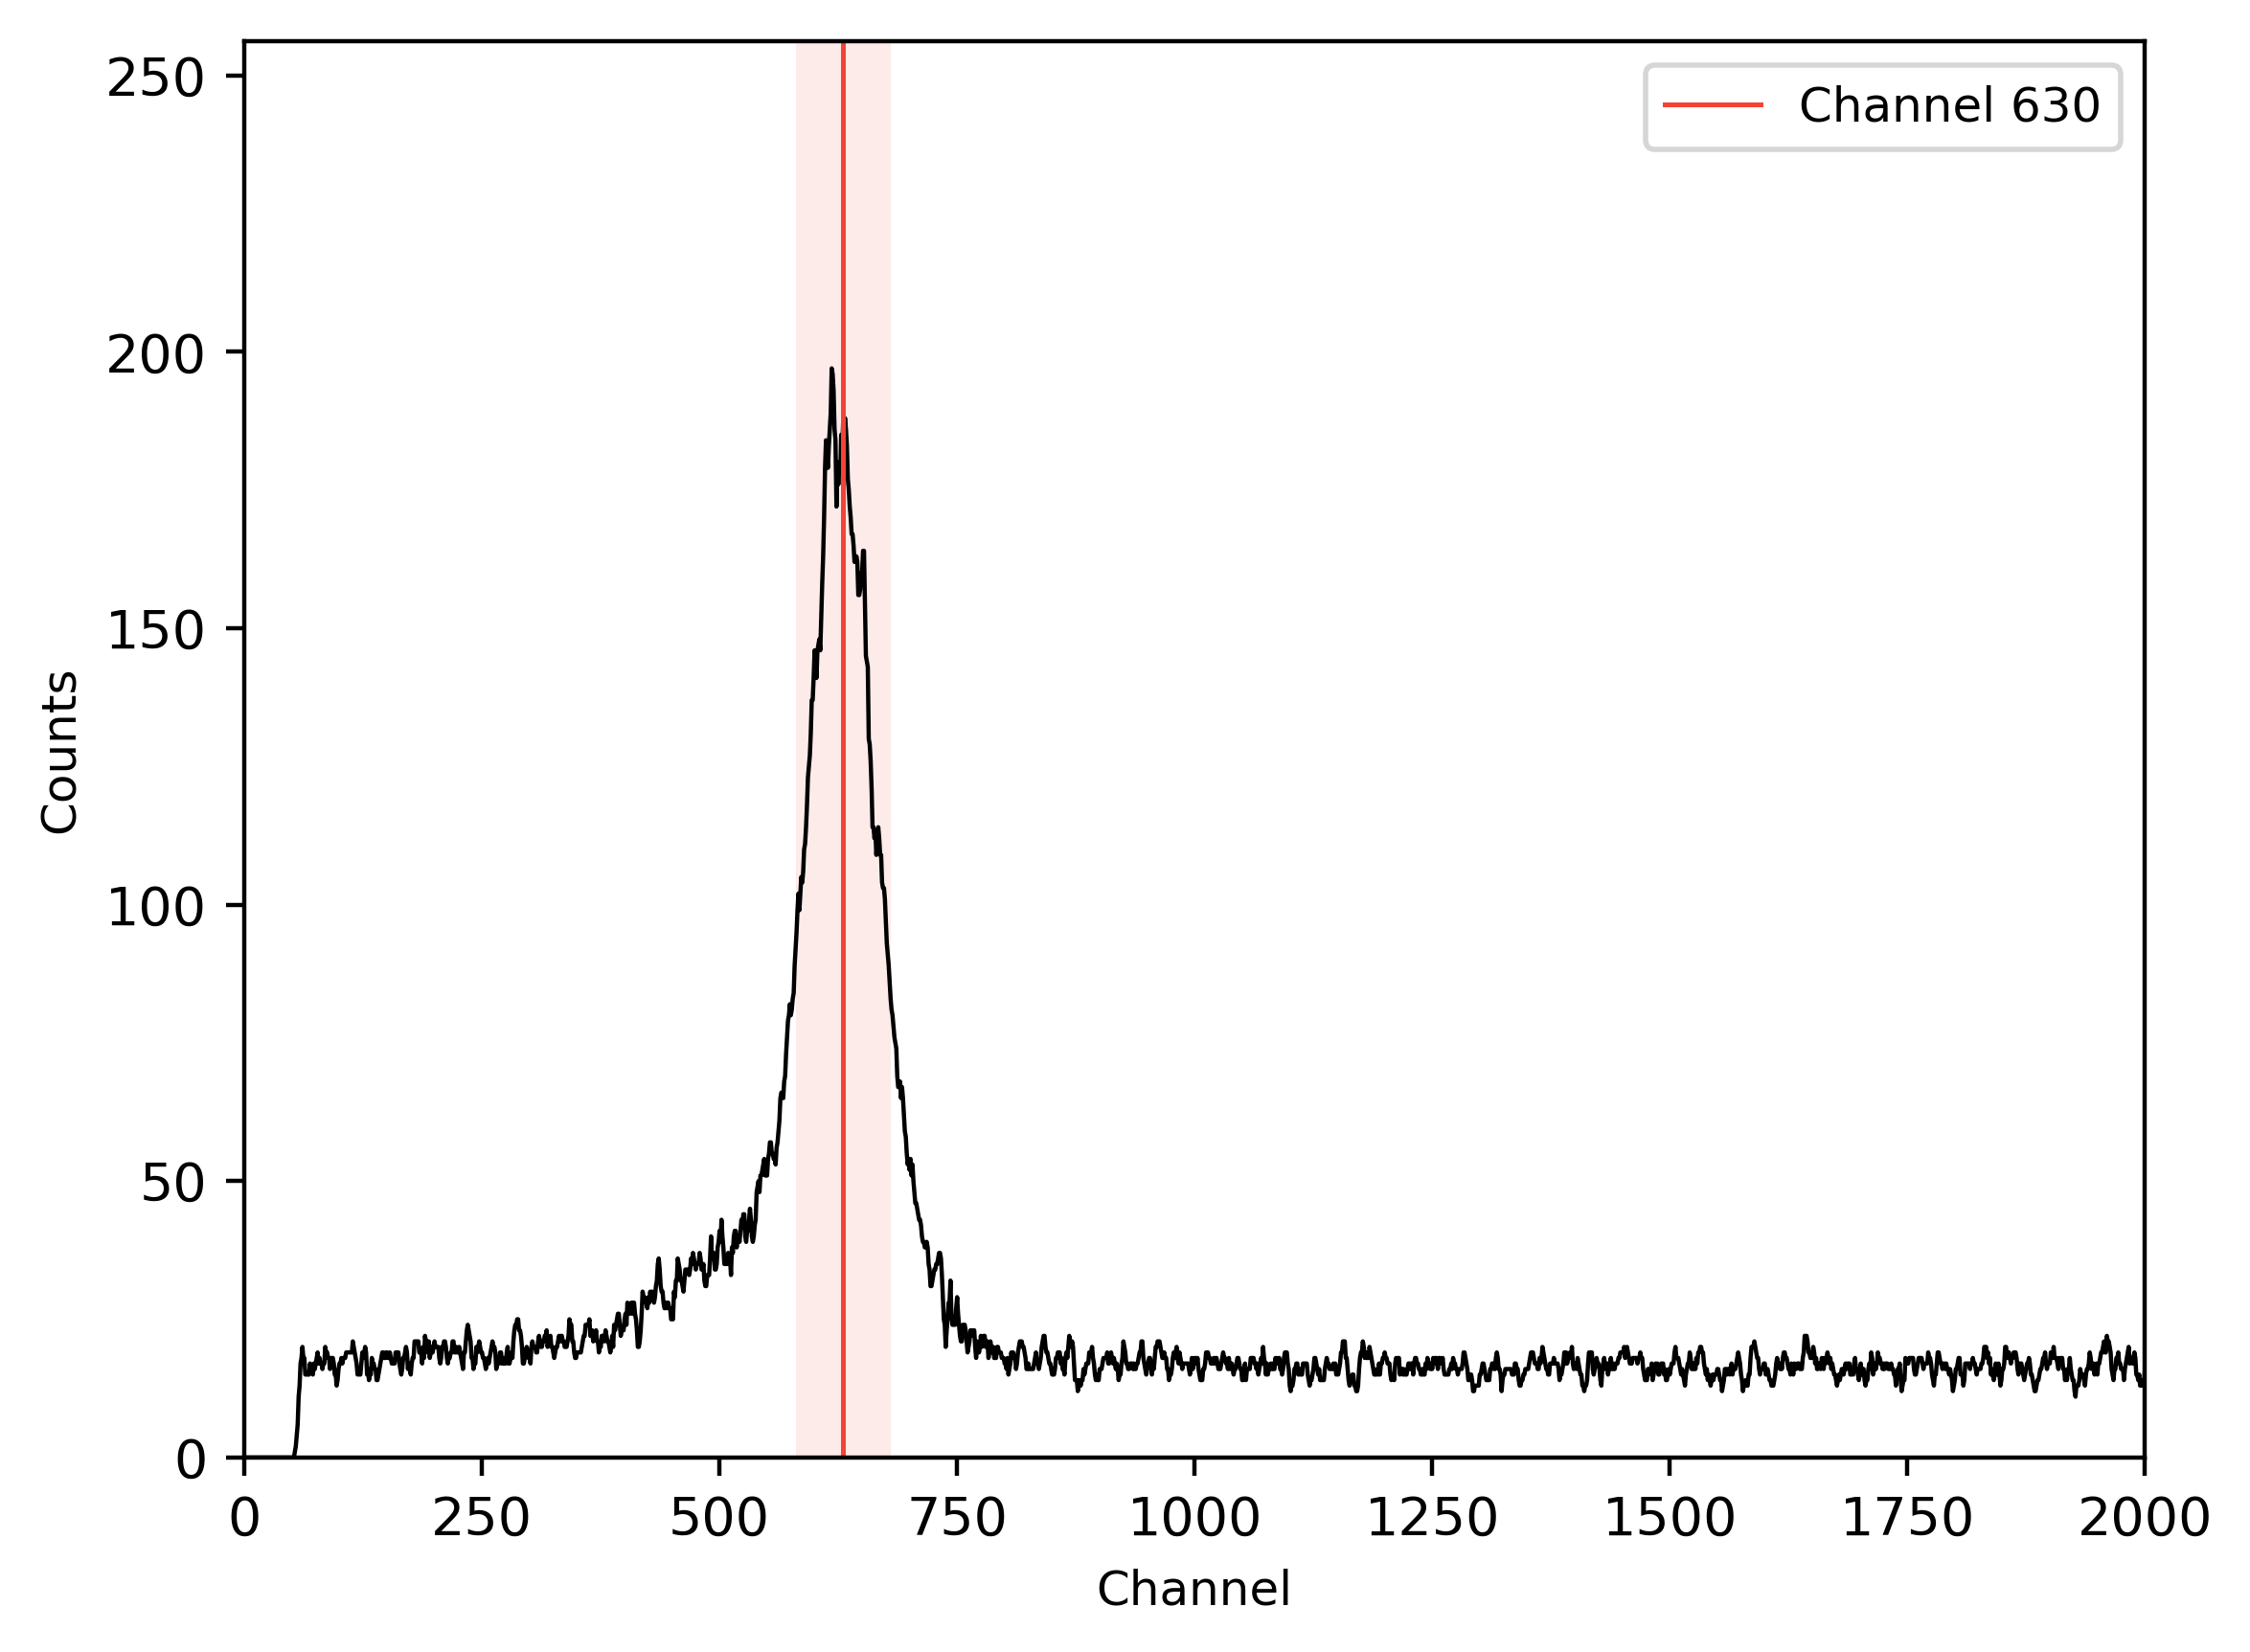
\includegraphics[]{png/137CsTPHC}
    \end{adjustbox}
    \captionof{figure}{137CsTPHC}
    \label{fig:}
\end{center}
%
\begin{center}
    \begin{adjustbox}{max width=\linewidth, keepaspectratio}
        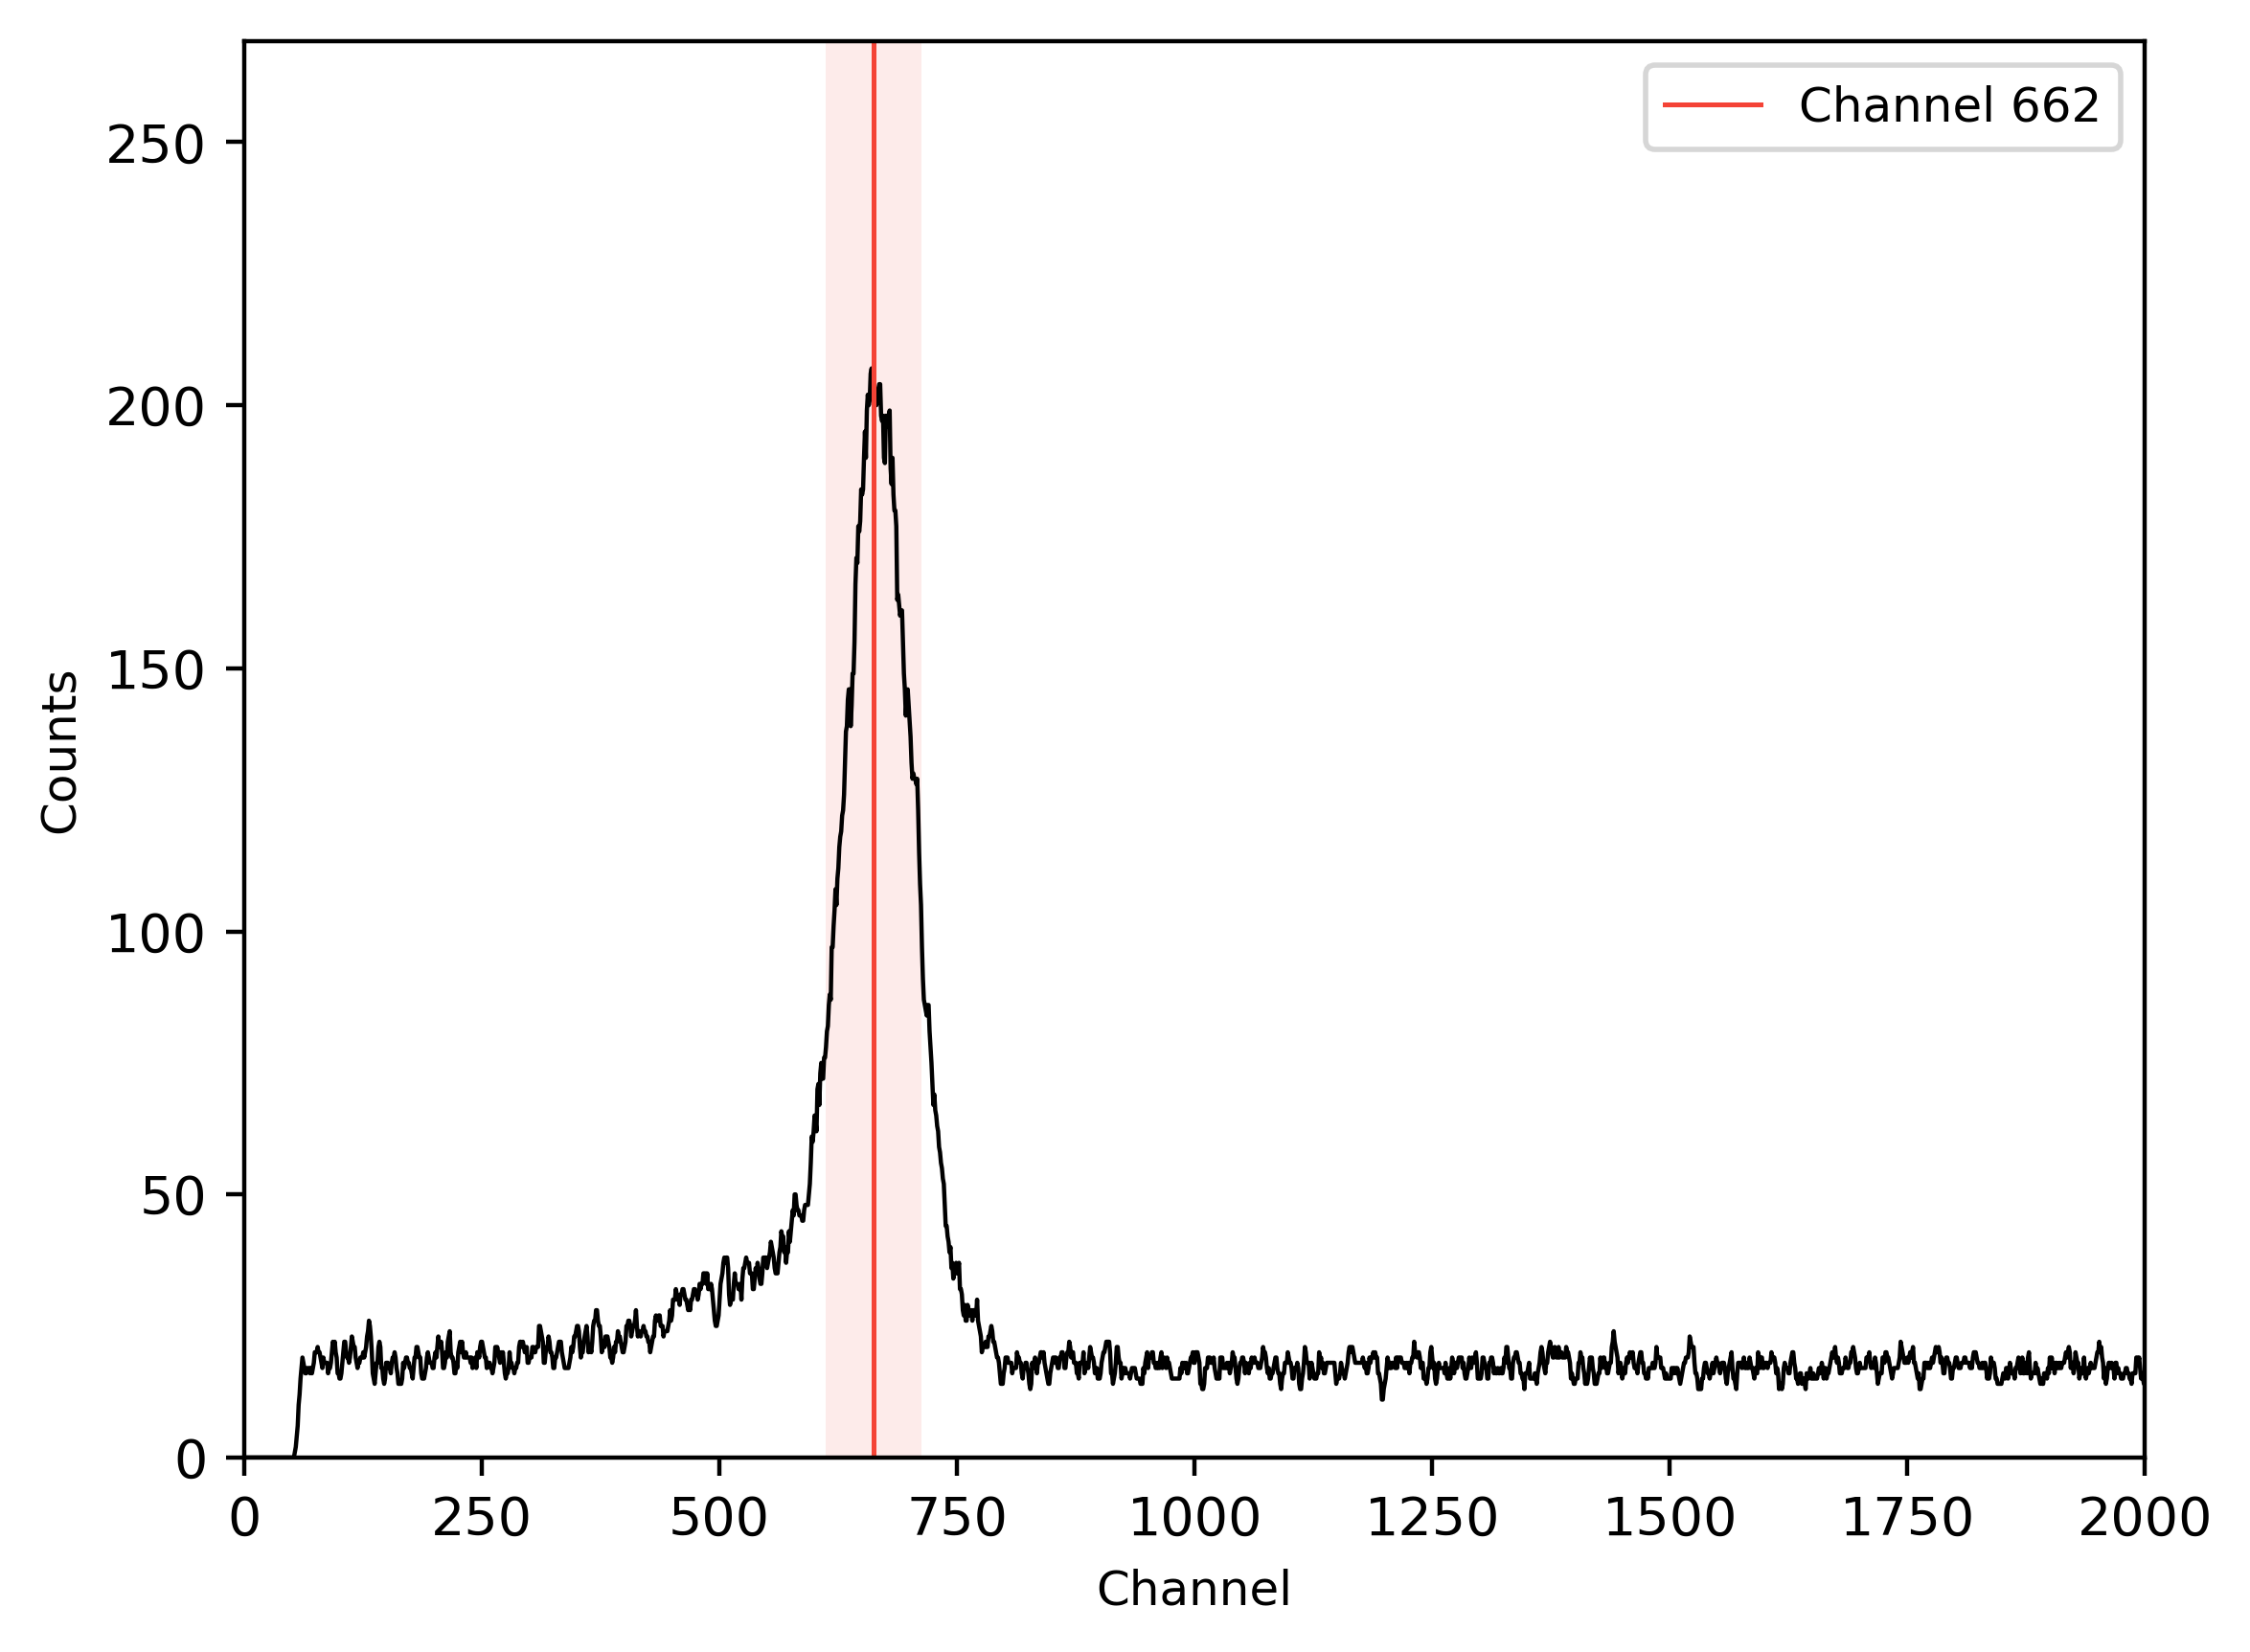
\includegraphics[]{png/137CsTPHC20ns}
    \end{adjustbox}
    \captionof{figure}{137CsTPHC20ns}
    \label{fig:}
\end{center}
%
\begin{center}
    \begin{adjustbox}{max width=\linewidth, keepaspectratio}
        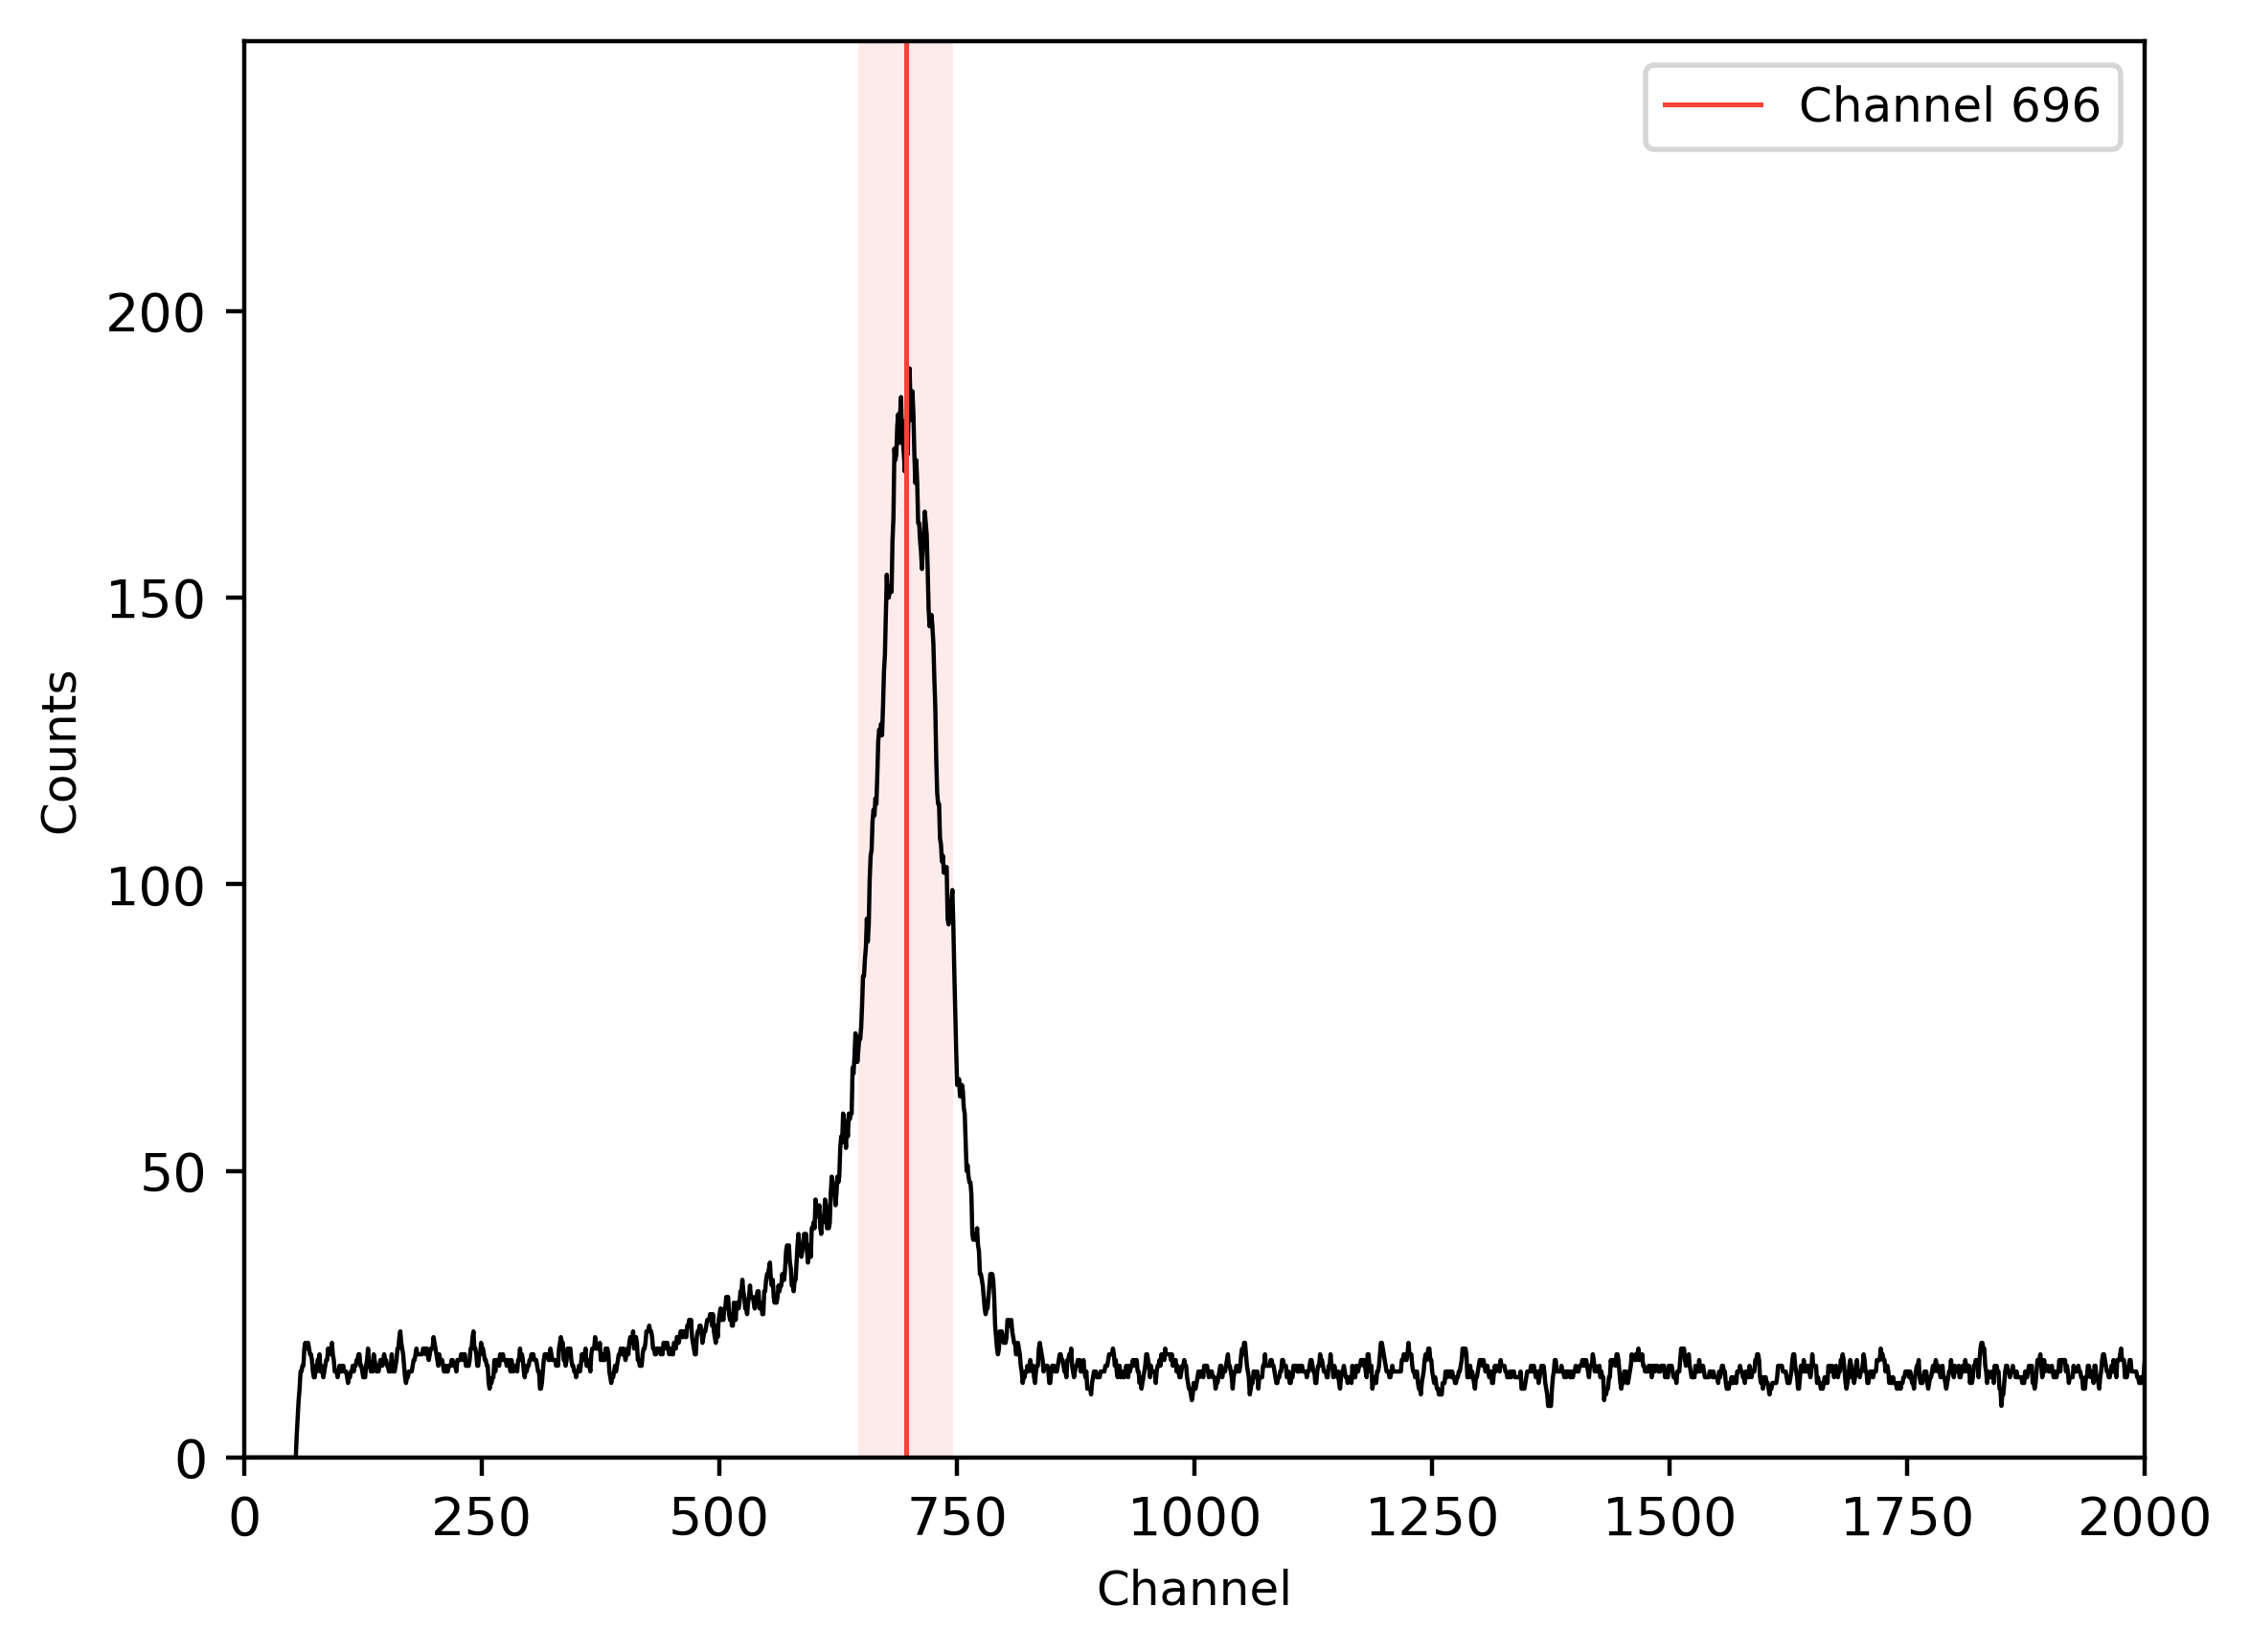
\includegraphics[]{png/137CsTPHC40ns}
    \end{adjustbox}
    \captionof{figure}{137CsTPHC40ns}
    \label{fig:}
\end{center}
%
\begin{center}
    \begin{adjustbox}{max width=\linewidth, keepaspectratio}
        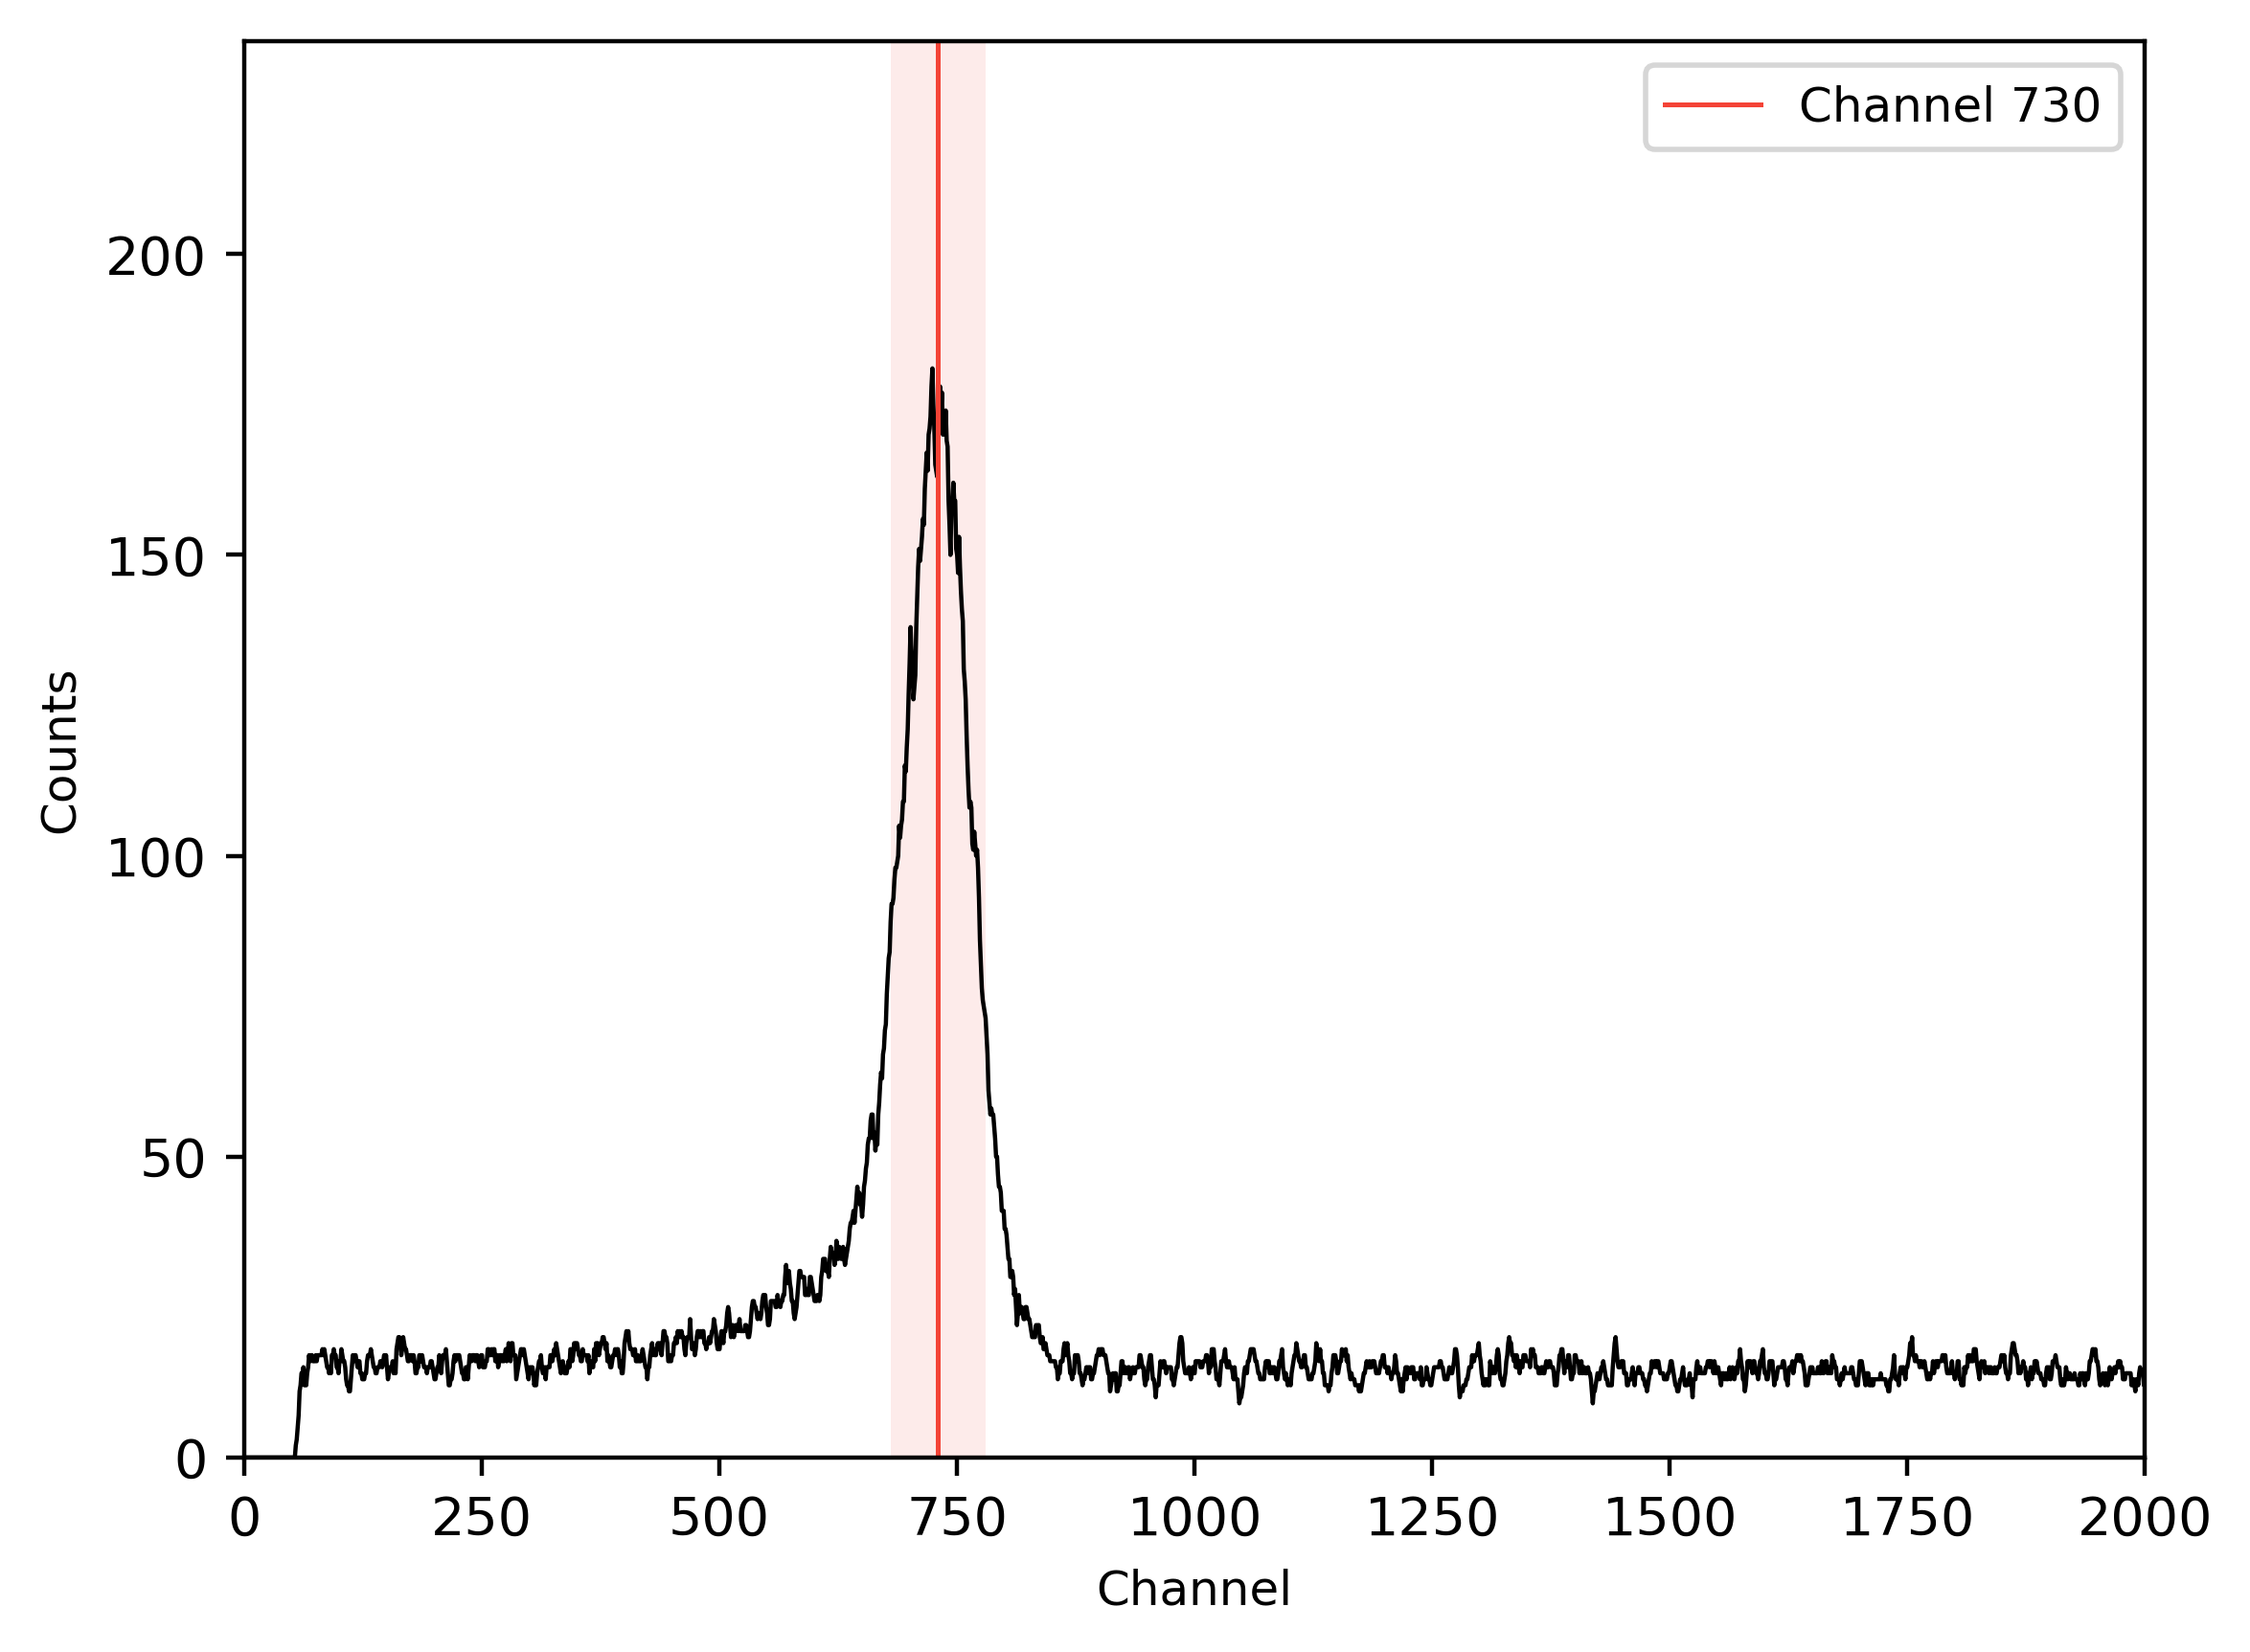
\includegraphics[]{png/137CsTPHC60ns}
    \end{adjustbox}
    \captionof{figure}{137CsTPHC60ns}
    \label{fig:}
\end{center}
%
\begin{center}
    \begin{adjustbox}{max width=\linewidth, keepaspectratio}
        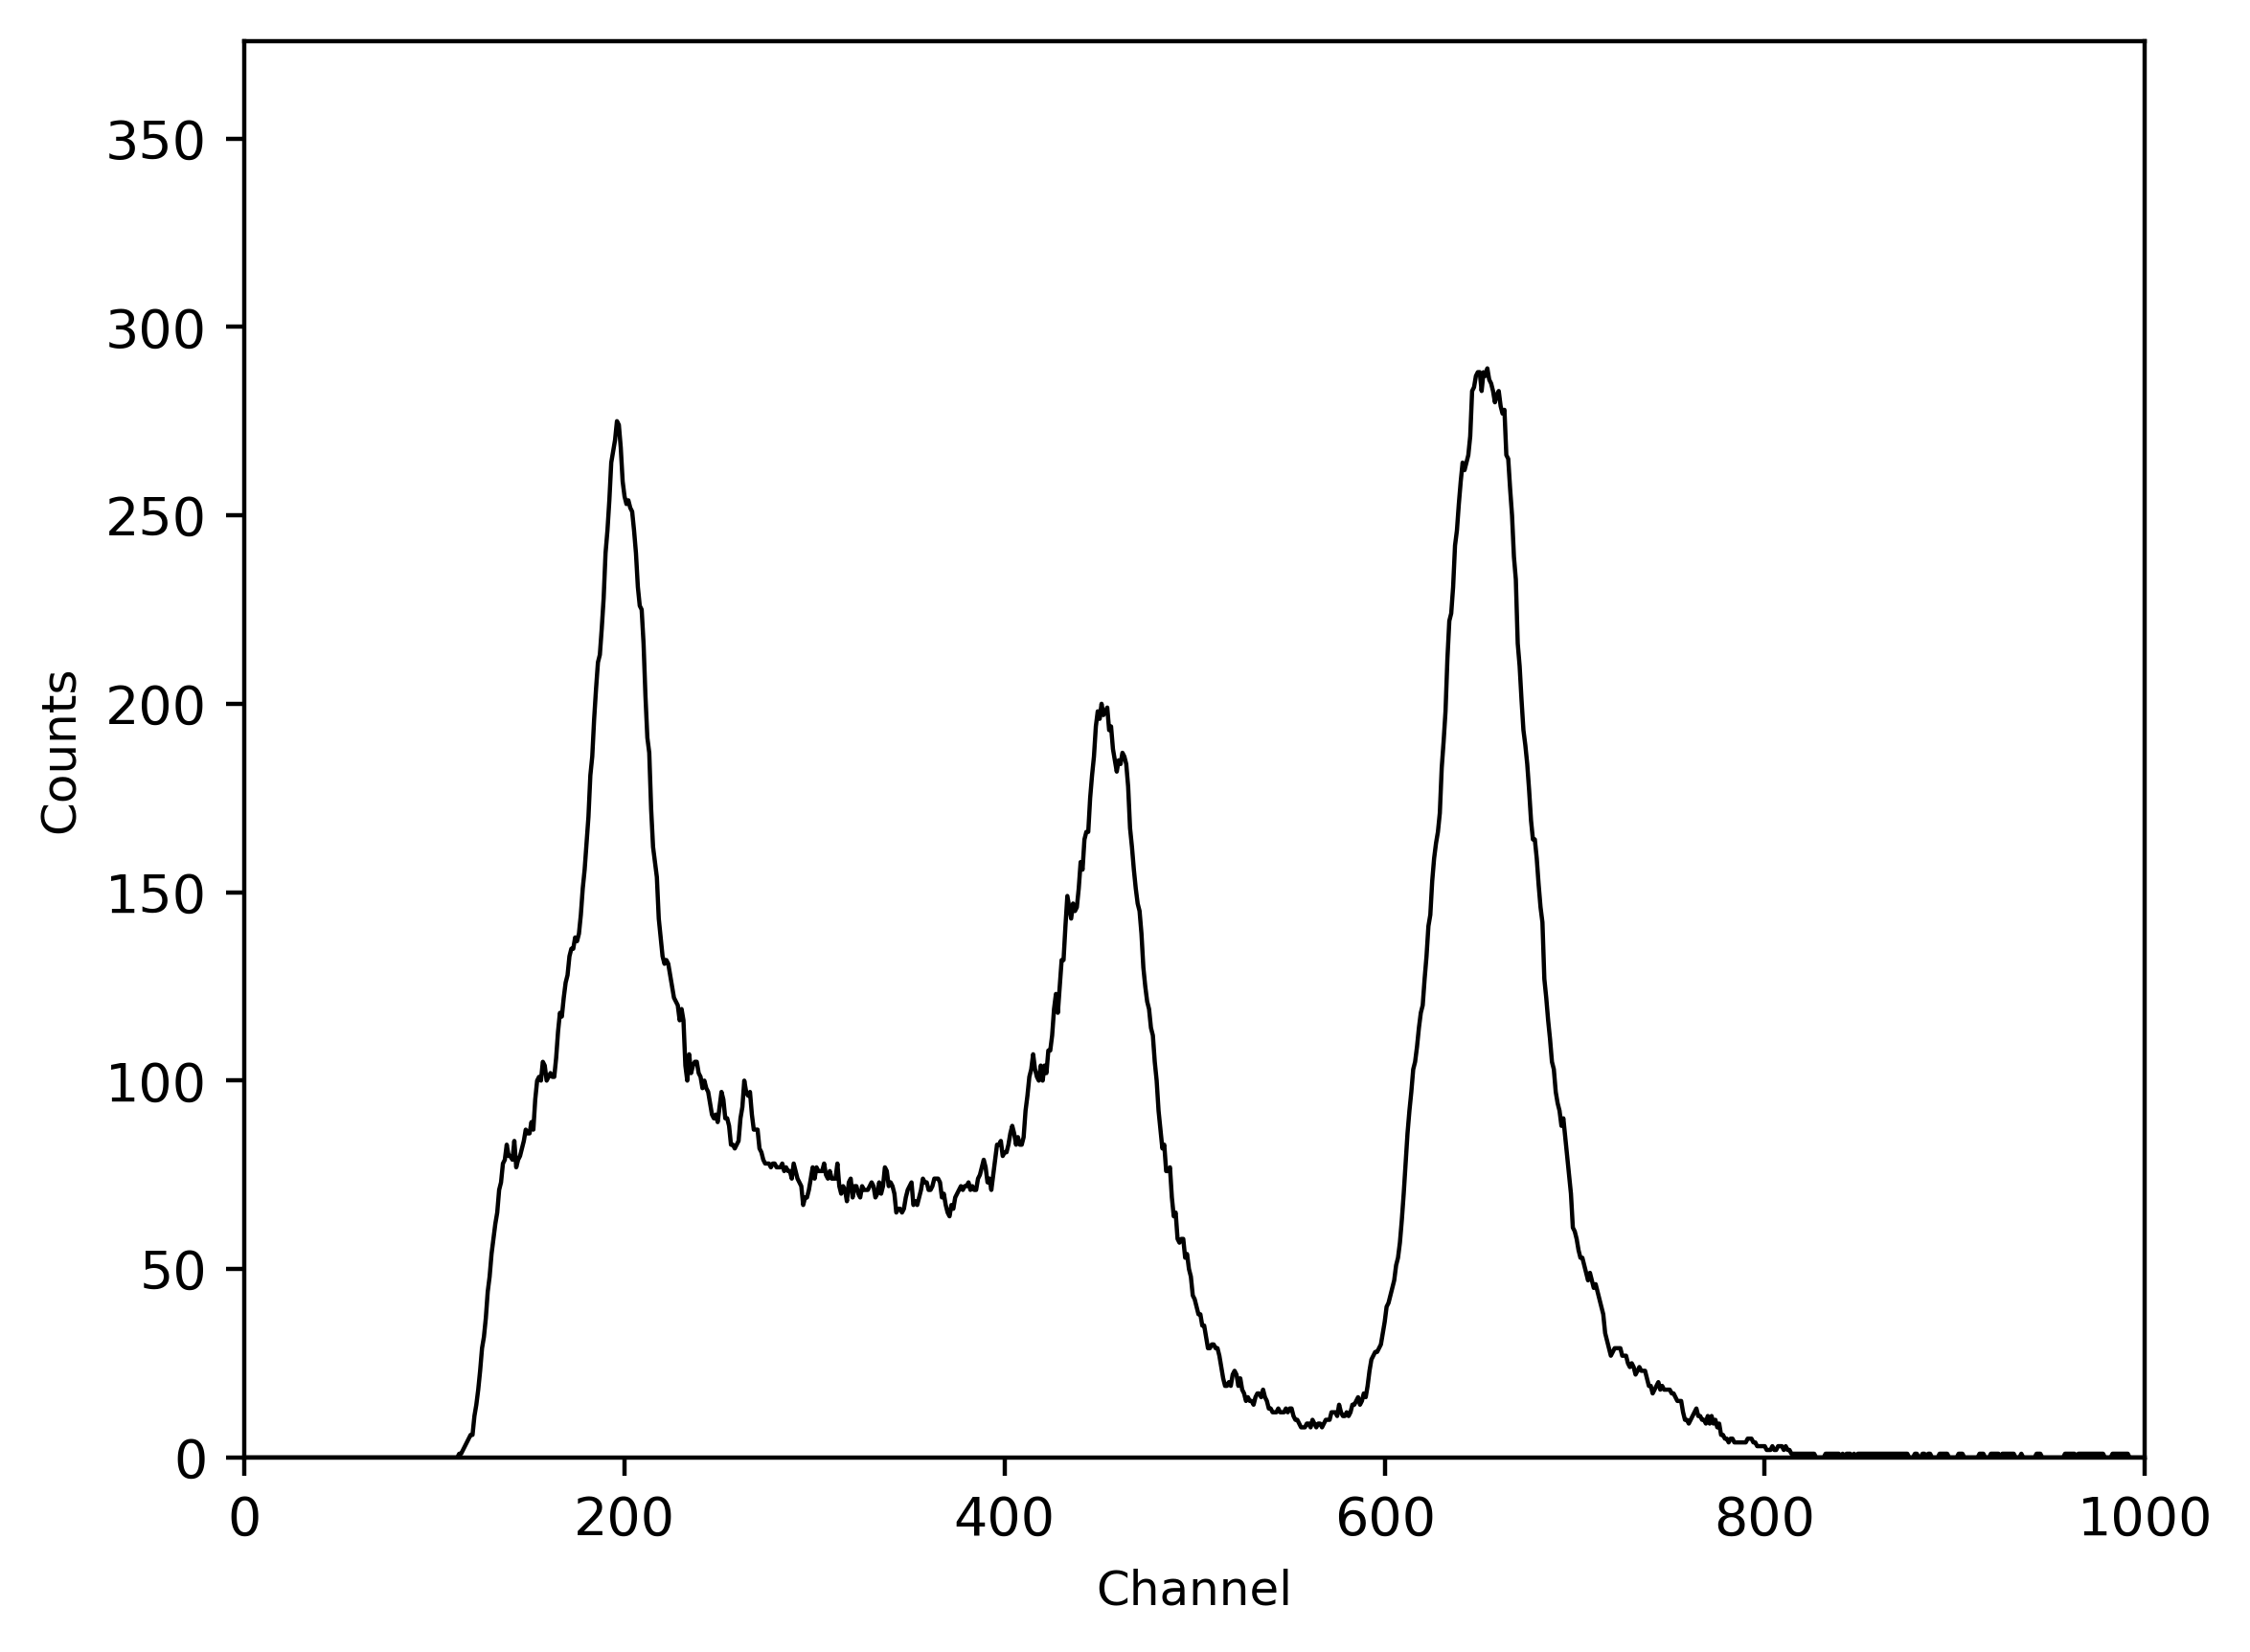
\includegraphics[]{png/137Cskoinz1}
    \end{adjustbox}
    \captionof{figure}{137Cskoinz1}
    \label{fig:}
\end{center}
%
\begin{center}
    \begin{adjustbox}{max width=\linewidth, keepaspectratio}
        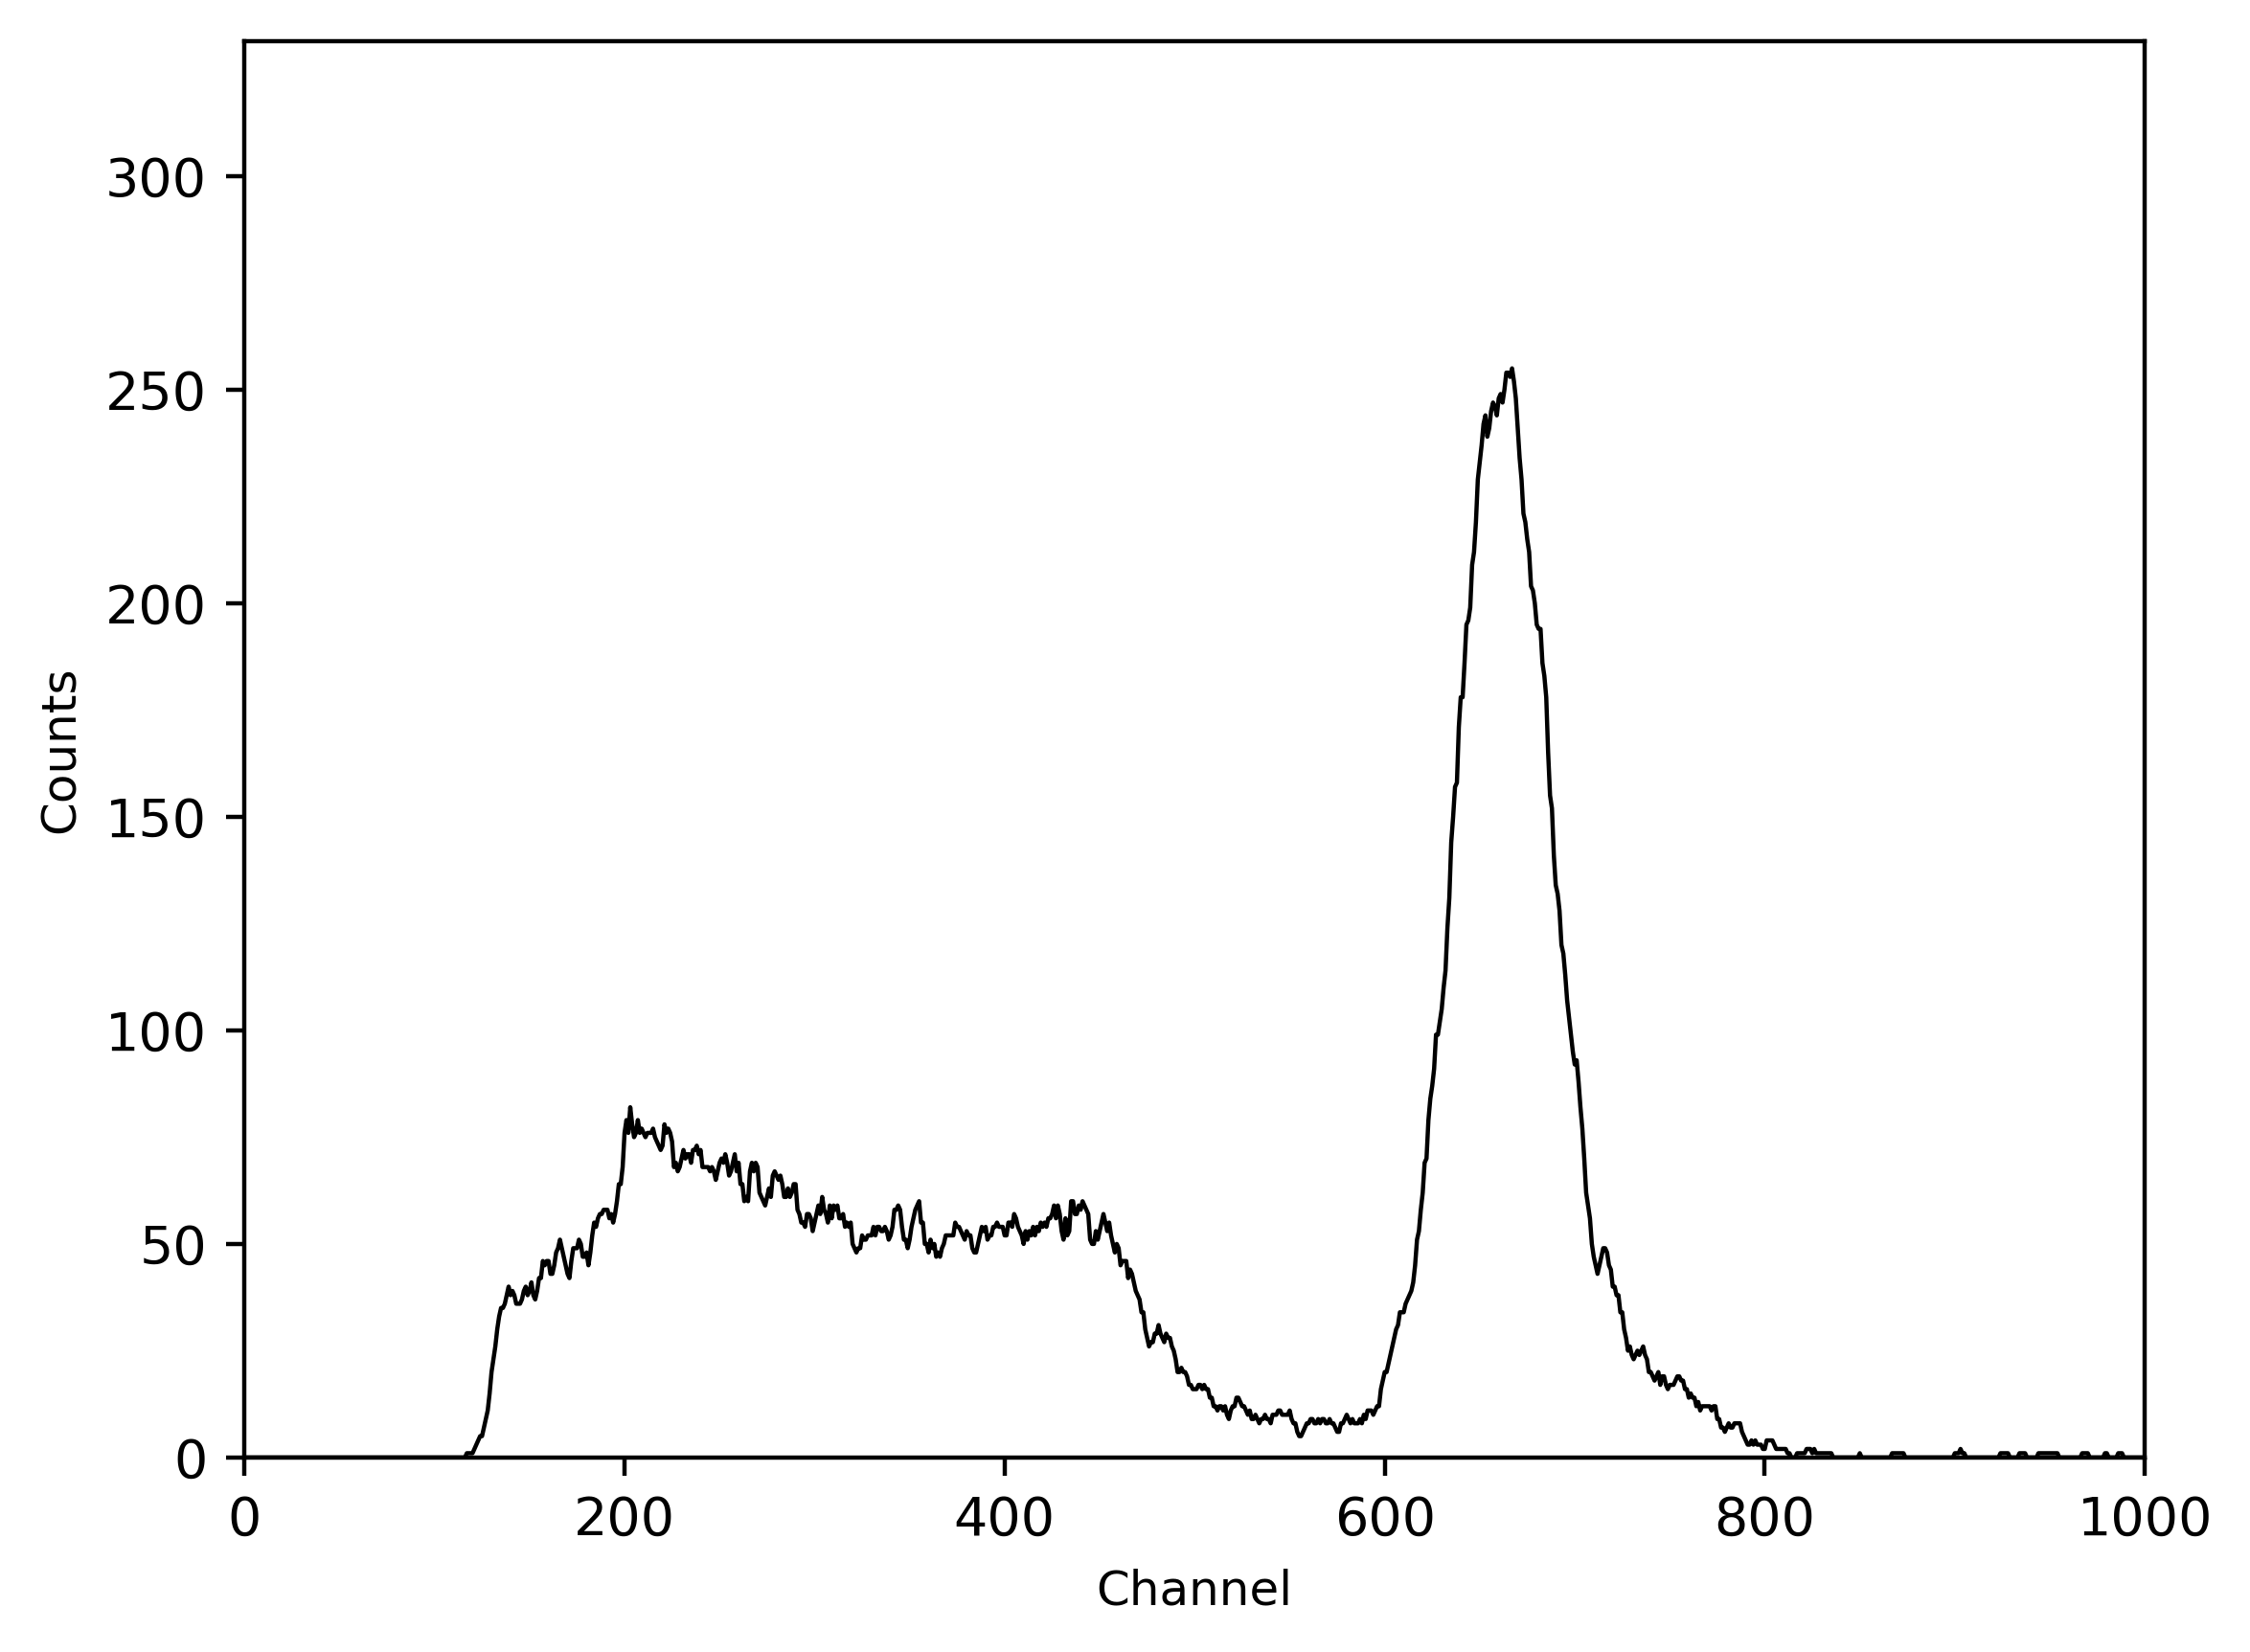
\includegraphics[]{png/137Cskoinz2}
    \end{adjustbox}
    \captionof{figure}{137Cskoinz2}
    \label{fig:}
\end{center}
%
\begin{center}
    \begin{adjustbox}{max width=\linewidth, keepaspectratio}
        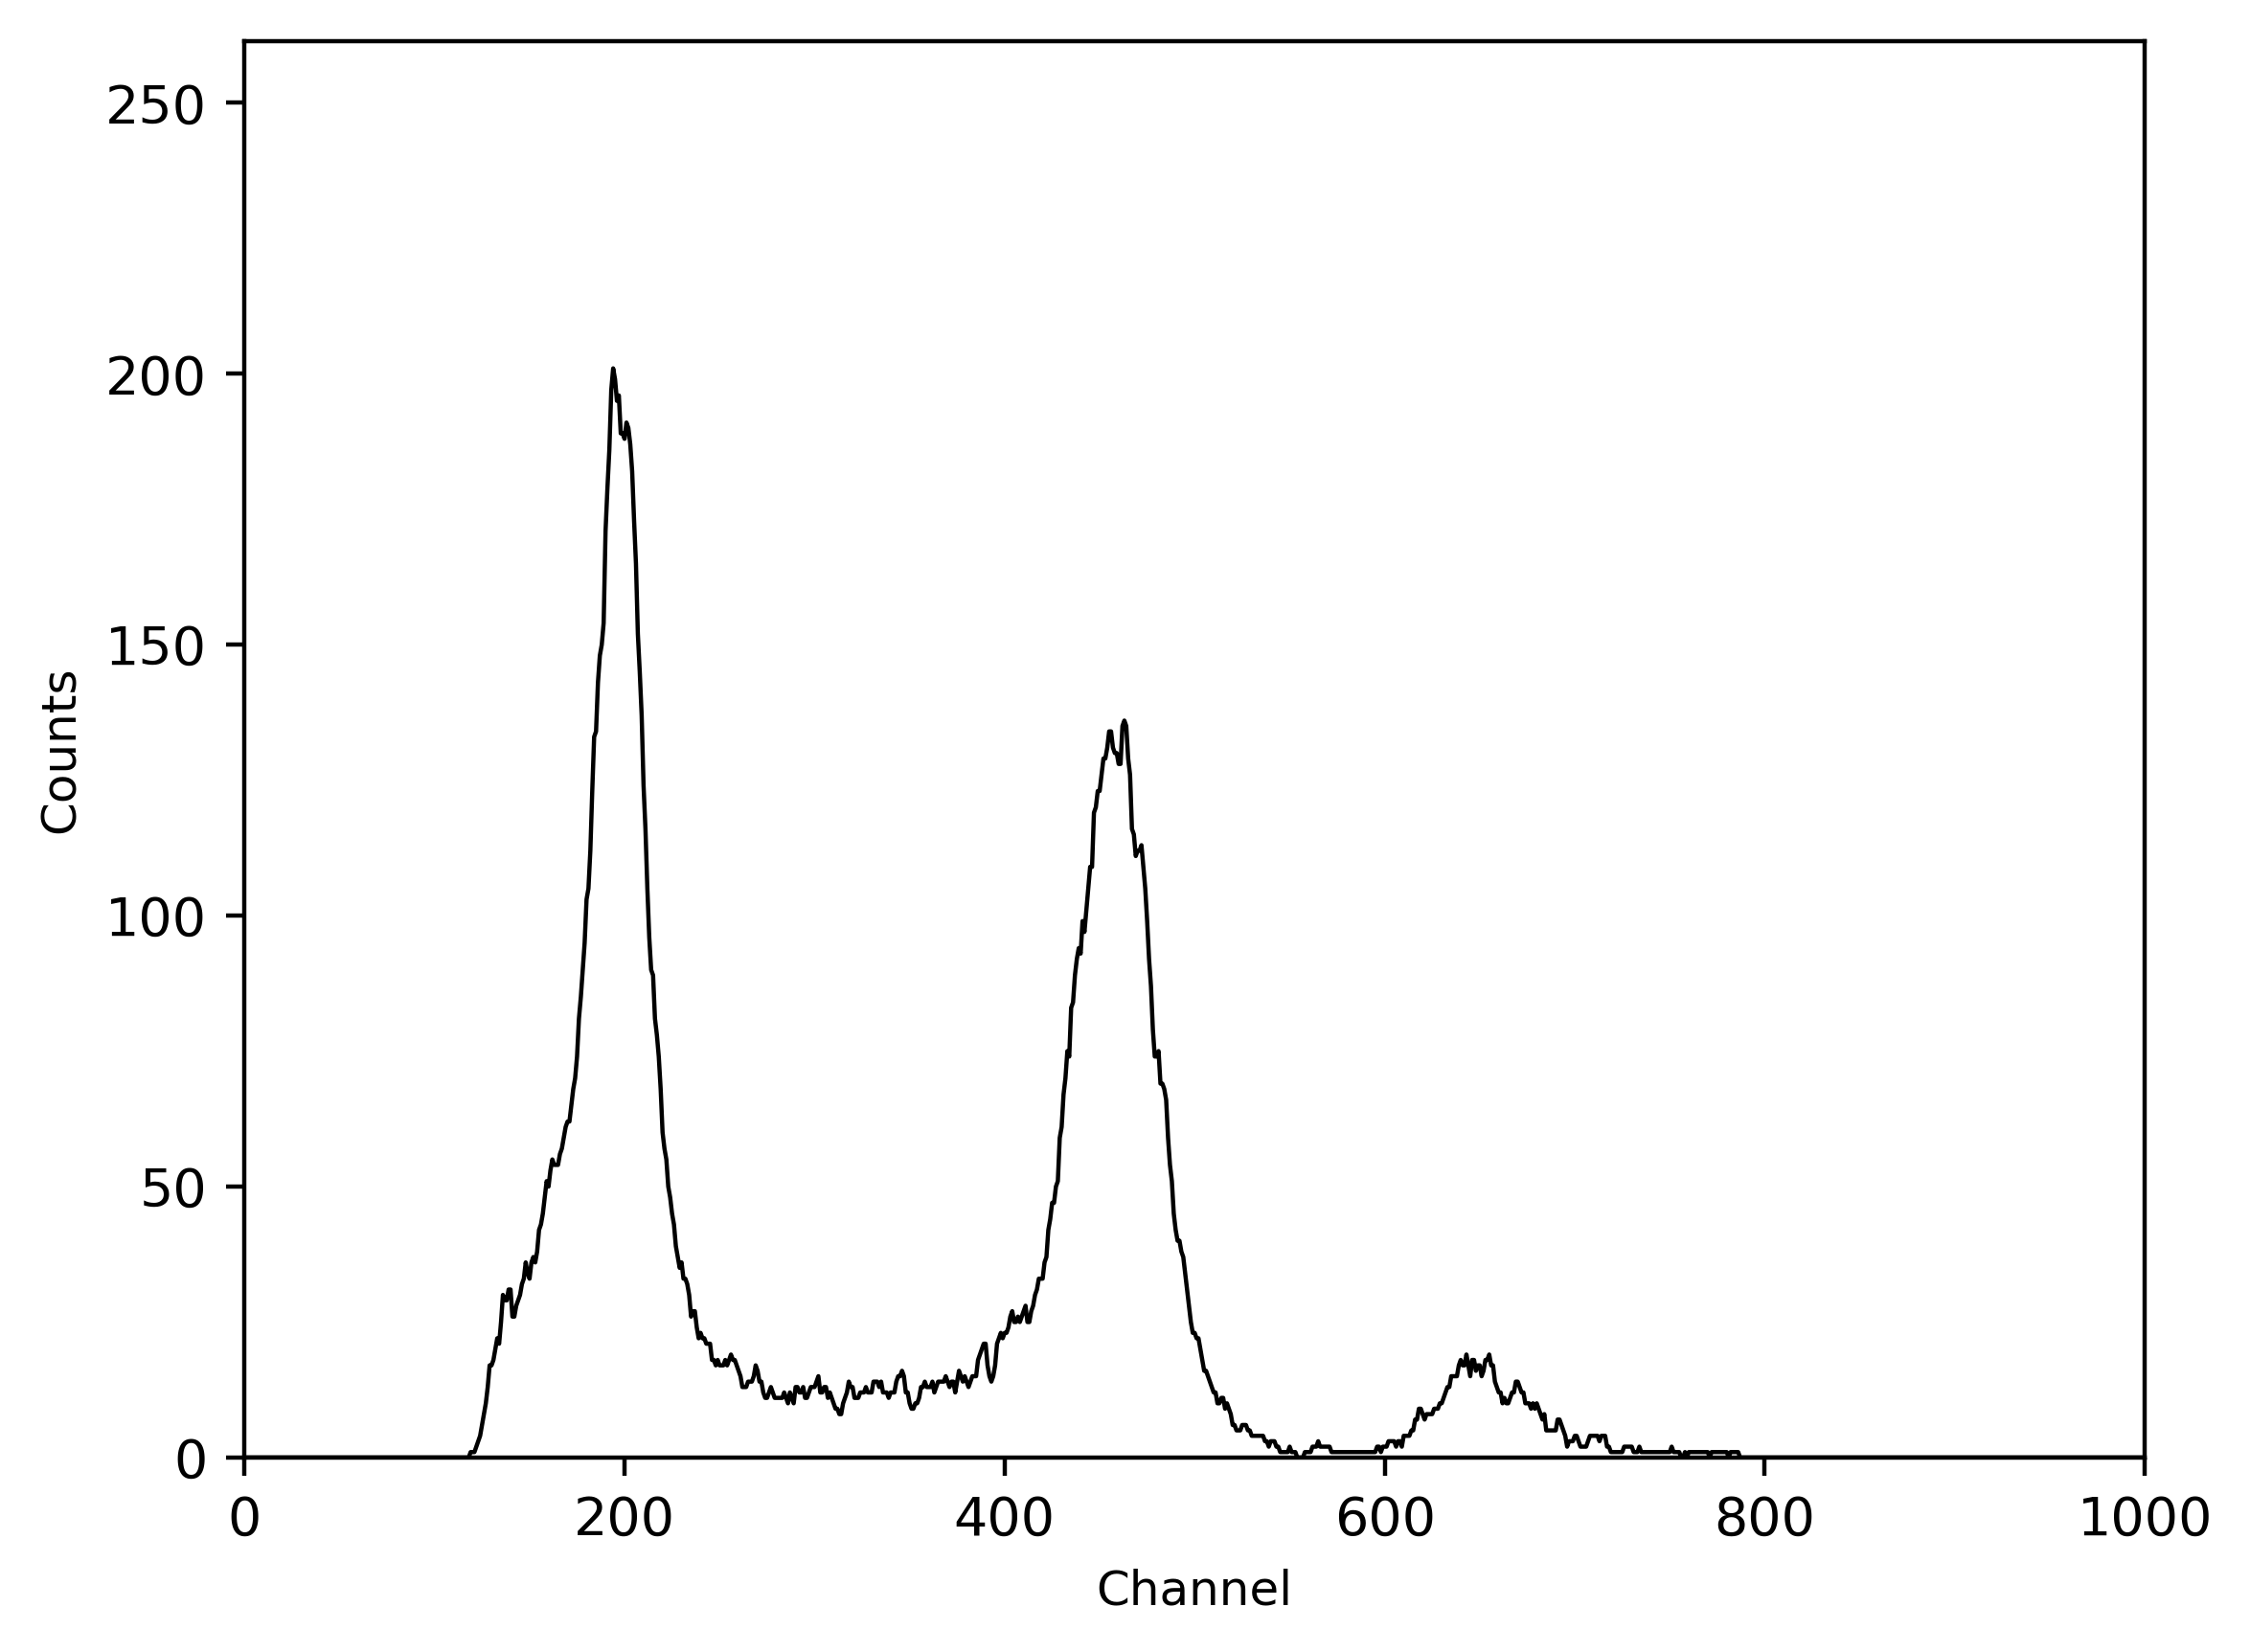
\includegraphics[]{png/137CsmitTPHC_gated}
    \end{adjustbox}
    \captionof{figure}{137CsmitTPHC\_gated}
    \label{fig:}
\end{center}
%
\begin{center}
    \begin{adjustbox}{max width=\linewidth, keepaspectratio}
        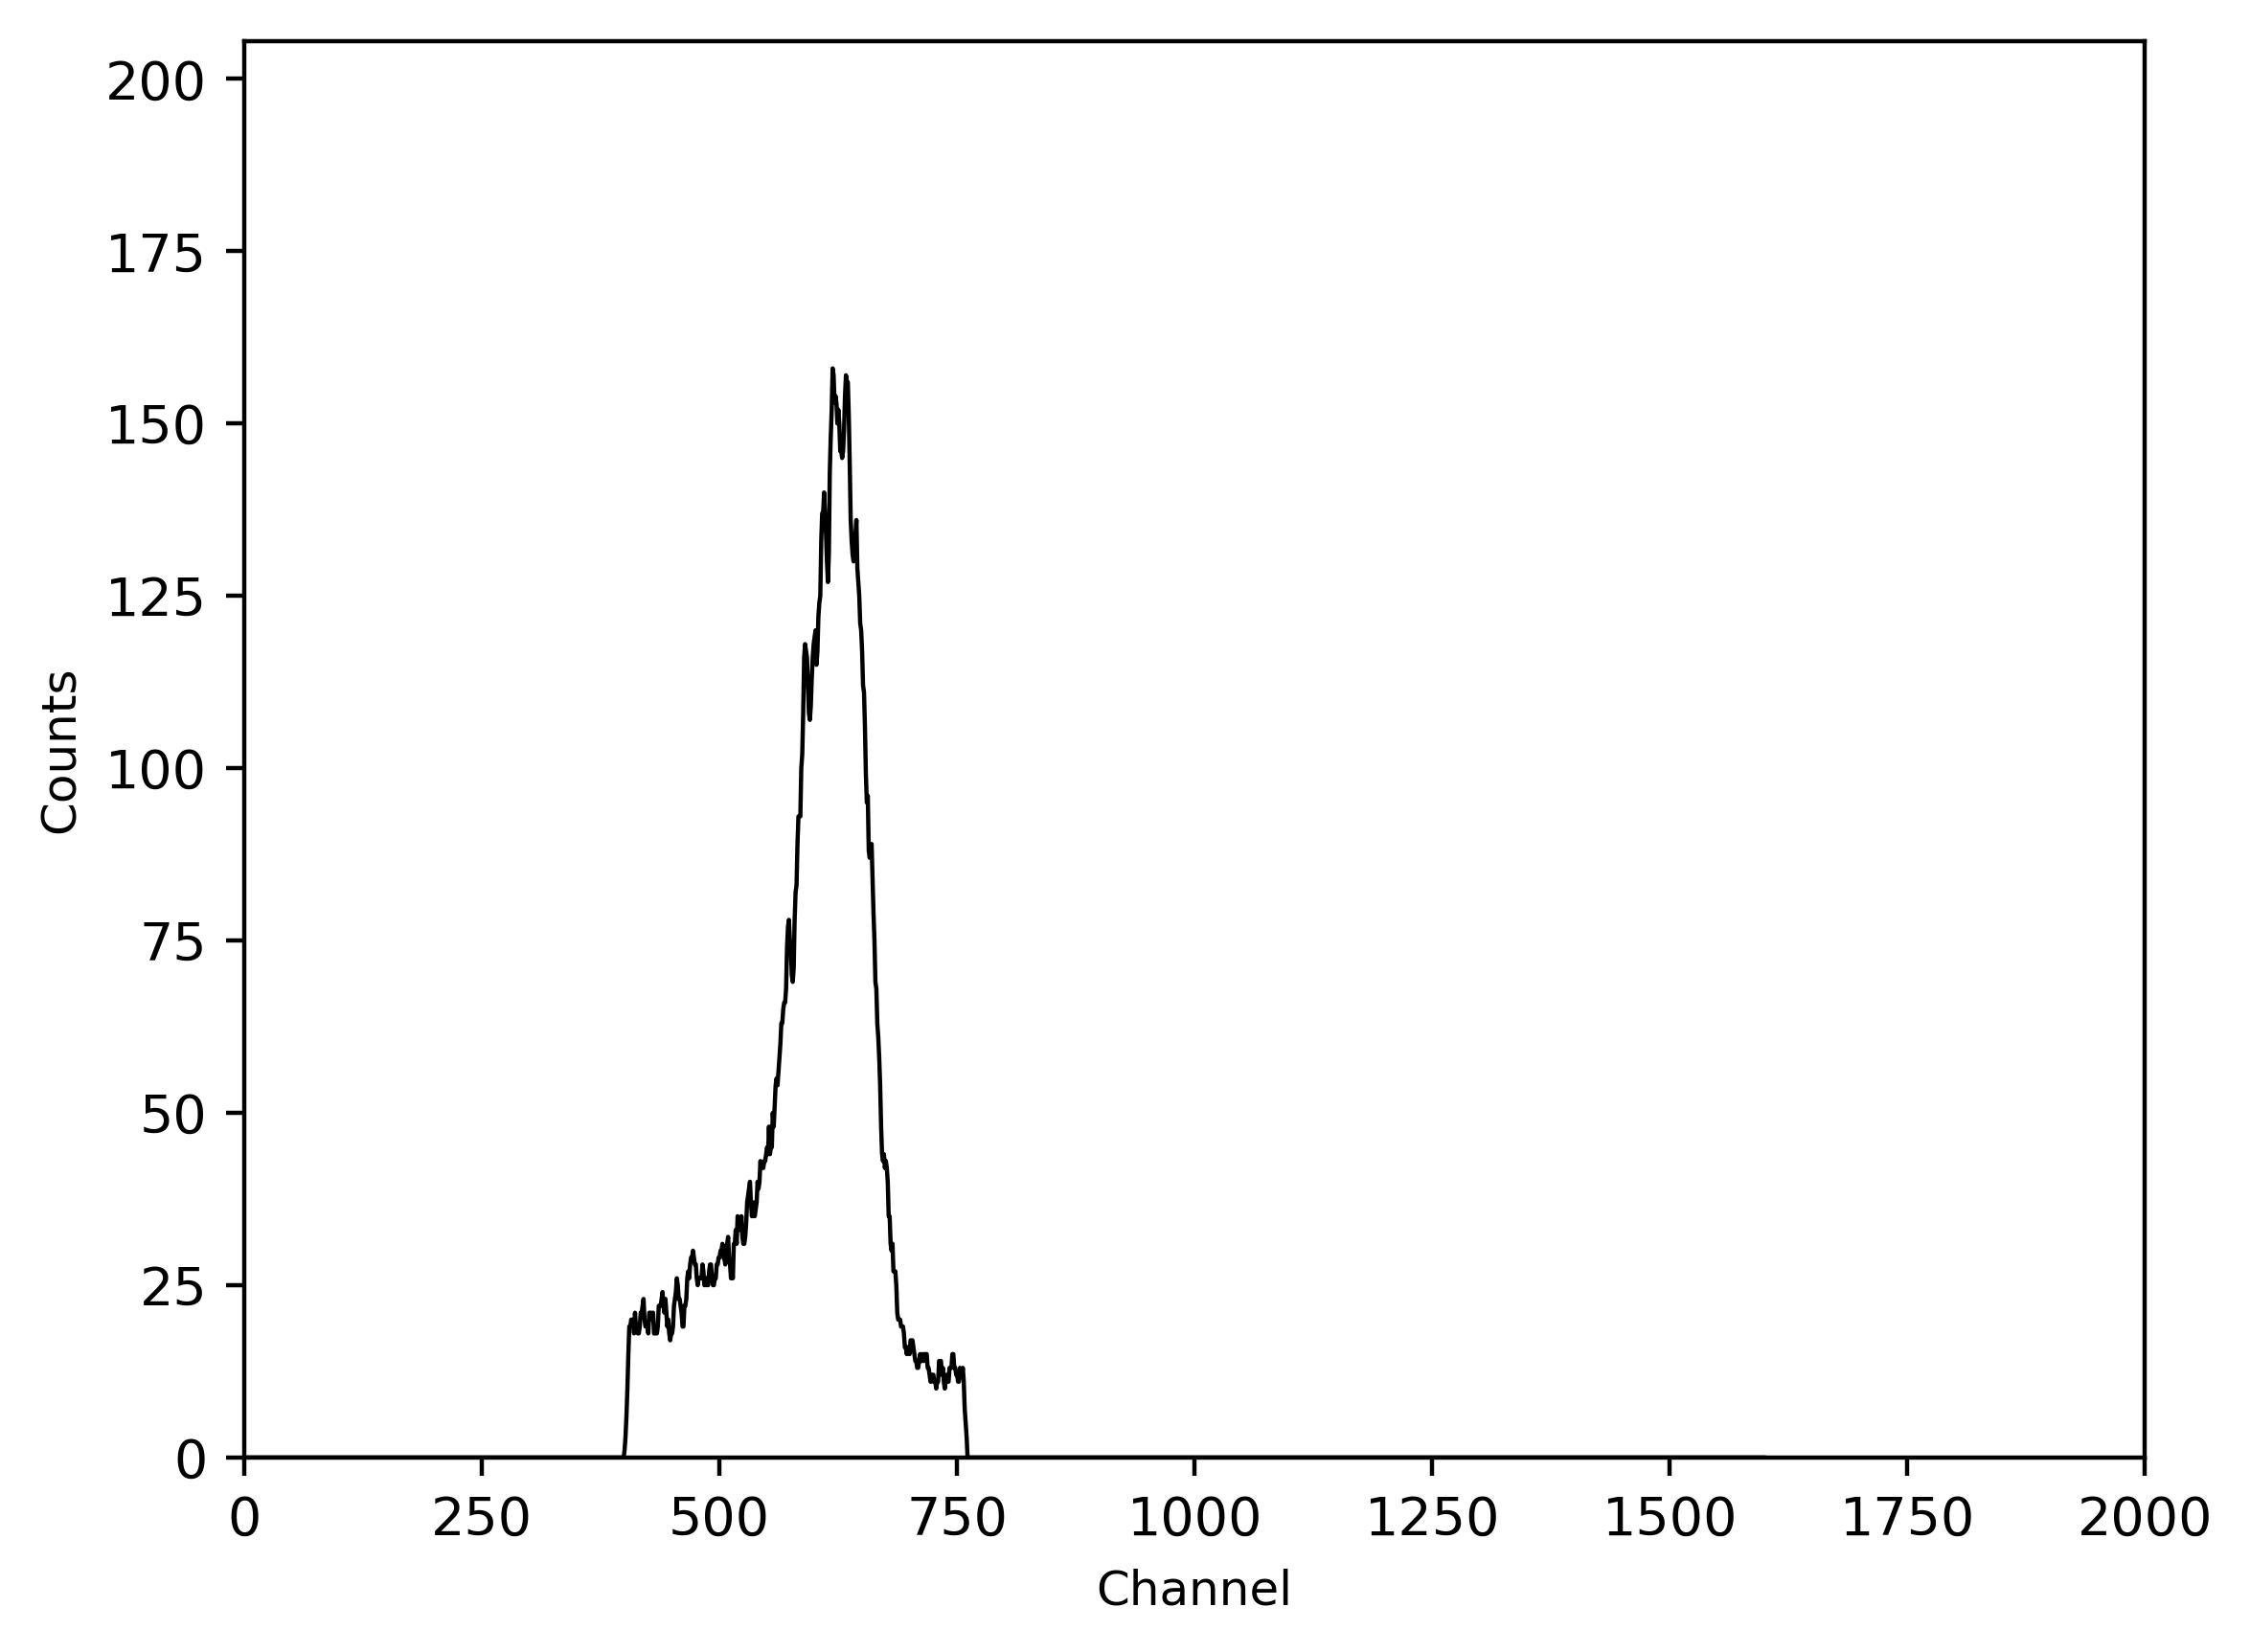
\includegraphics[]{png/137CsTPHC_geschnitten_neu}
    \end{adjustbox}
    \captionof{figure}{137CsTPHC\_geschnitten\_neu}
    \label{fig:}
\end{center}
